\begingroup

\let\clearpage\relax

\chapter{Learning Algorithms for Rested Markovian Bandits}
\label{ch:learning_rested}

In this chapter, we study the scalability of model-based algorithms learning the optimal policy of a discounted rested Markovian bandit problem with $n$ arms. % There are two categories of model-based reinforcement learning algorithms: Bayesian algorithms (like PSRL), and optimistic algorithms (like UCRL2 or UCBVI).
%In this chapter, 
We construct variants of three algorithms specially tailored to Markovian bandits (MB) that we call MB-PSRL, MB-UCRL2, and MB-UCBVI. We consider an episodic setting with geometrically distributed episode length, and measure the performance of the algorithm in terms of regret (Bayesian regret for MB-PSRL and expected regret for MB-UCRL2 and MB-UCBVI). We prove that, for this setting, all algorithms have a low regret in $\tilde{\landauO}(S\sqrt{nK})$ -- where $K$ is the number of episodes, $n$ is the number of arms and $S$ is the number of states of each arm. Up to a factor $\sqrt{S}$, these regrets match the Bayesian minimax regret lower bound of $\Omega(\sqrt{SnK})$ that we also derive.

Even if their theoretical regrets are comparable, the \emph{time complexities} of these algorithms vary greatly: We show that MB-UCRL2, as well as all optmistic algorithms that use confidence bonuses on transition matrices have a {time} complexity that grows exponentially in $n$. In contrast, MB-UCBVI does not use bonuses on transition matrices, and we show that  it can be implemented efficiently, with a time complexity linear in $n$. Our numerical experiments show, however, that its empirical regret is large. Our Bayesian algorithm, MB-PSRL, enjoys the best of both worlds: its running time is linear in the number of arms and its empirical regret is the smallest of all algorithms.
This is a new addition in the understanding of the power of Bayesian algorithms, that can often be  tailored to the structure of the problems to learn.

In Section~\ref{ch:rested:sec:contribute}, we summarize our result in learning with rested Markovian bandit with discount.
Section~\ref{ch:rested:related} describes the work in learning with structured MDPs such as factored MDPs, and rested bandit with no discount.
We recall the formulation of rested bandit problem with discount in Section~\ref{ch:rested:sec:bandits}.
Section~\ref{ch:rested:sec:problem} contains the episodic learning setup in which the episode length is geometrically distributed.
We present the modification of PSRL, UCRL2, and UCBVI to rested bandit with discount in Section~\ref{ch:rested:sec:learning_algorithms}.
We provide the analysis of their regret in Section~\ref{ch:rested:sec:analysis}.
Section~\ref{ch:rested:scale} contains our discussion on the scalability of each algorithm.
We report numerical evidences about the learning performance and the runtime of each algorithm in Section~\ref{ch:rested:sec:numerical}.
Section~\ref{ch:rested:sec:conclusion} summarizes the theoretical and numerical results of the modified algorithms and concludes the chapter.

\section{Contribution}
\label{ch:rested:sec:contribute}

We consider an episodic setting with geometrically distributed episode length, in which the optimal strategy for a decision maker who knows all parameters of the system is to use Gittins index policy. We study a specialization of PSRL \cite{osband2013more} to Markovian bandits, that we call Markovian bandit posterior sampling (MB-PSRL) that consists in using PSRL with a prior tailored to Markovian bandits. We show that the Bayesian regret of MB-PSRL is sublinear in the number of episodes and arms. We also provide an expected regret guarantee for two optimistic algorithms that we call MB-UCRL2 and MB-UCBVI, and that are based respectively on UCRL2 \cite{jaksch2010near} and UCBVI \cite{azar2017minimax}. They both use modified  confidence bounds adapted to Markovian bandit problems. The upper bound for their regret is similar to the bound for MB-PSRL. This shows that in terms of regret, the Bayesian approach (MB-PSRL) and the optimistic approach (MB-UCRL2 and MB-UCBVI) scale well with the number of arms. We also provide a Bayesian minimax regret lower bound for any learning algorithm in rested Markovian bandit problems with the aforementioned setting, which shows that the regret bounds that we obtain for the three algorithms are close to optimal.

The situation is radically different when considering the processing time: the runtime of MB-PSRL is linear (in the number of arms), while the runtime of MB-UCRL2 is exponential. We show that this is not an artifact of our implementation of MB-UCRL2 by exhibiting a Markovian bandit problem for which being optimistic in each arm is not optimistic in the global MDP. This implies that UCRL2 and its variants \cite{bourel2020tightening,fruit2018efficient,talebi2018variance,filippi2010optimism} cannot be adapted to have efficient runtime in Markovian bandit problems unless an oracle gives the optimistic policy. We argue that this non-scalability of UCRL2 and its variants is not a limitation  of the optimistic approach but comes from the fact that UCRL2 relies on  extended value iteration \cite{jaksch2010near} needed to deal with  upper confidence bounds on the transition matrices.  We show that MB-UCBVI, an optimistic algorithm that does not add bonus on transition probabilities and hence does not rely on extended value iteration,  does not suffer from the same problem. Its  regret is  sublinear in the number of episodes, and arms (although larger than the regret of both MB-PSRL and MB-UCRL2), and its  runtime is linear in the number of arms.
This allows us to conclude that, on the one hand, if a weakly coupled MDP or a factored MDP can be solved efficiently when all the parameters are known, then the Bayesian approach is efficient both in terms of learning and computation time. On the other hand, knowing how to solve a weakly coupled MDP or a factored MDP efficiently is not sufficient for all optimistic algorithms to be computationally efficient.

We also conduct a series of numerical experiments to compare the performance of MB-PSRL,  MB-UCRL2 and MB-UCBVI.  They confirm the good behavior of MB-PSRL, both in terms of regret and computational complexity. These numerical experiments also show that the empirical regret of MB-UCBVI is larger than the regret of MB-PSRL and MB-UCRL2, confirming the comparisons between the upper bounds derived in Theorem \ref{thm:regret_upper_bound}. All this  makes MB-PSRL the better choice between the three learning algorithms.

\section{Related work}
\label{ch:rested:related}

Markovian bandits have been applied to many problems such as single-machine scheduling, choosing a job in  resource constraint problems  as well as other  industrial research problems. Many applications can be found in \cite[Section 3.6]{puterman2014markov} and \cite{gittins2011multi}. \cite{gittins1979bandit} shows that discounted rested Markovian bandit can be solved linearly in the number of arms using Gittins index policy. Therefore, several papers are   focused  on the complexity of  computing  Gittins index \cite{chakravorty2014multi,gast2022computing}.
In this chapter, we focus on rested Markovian bandit problems with discount factor $\gamma<1$ where all
reward functions and transition matrices are unknown.
A possible approach to learn under these conditions is to ignore the problem's structure and view the Markovian bandit problem as a generic MDP.
As we have seen in Chapter~\ref{ch:rl}, there are two main families of model-based general-purpose RL algorithms with regret guarantee. The first one uses the \emph{optimism in face of uncertainty} (OFU) principle and the second family uses a Bayesian approach, the posterior sampling method introduced by \cite{thompson1933likelihood}.
Yet, applied as-is to Markovian bandit problems, these bounds grow exponentially with the number of arms.

Our work is not the first attempt to exploit the structure of an MDP to improve
learning.  Factored MDPs (the state space can be
factored into $n\in\mathbb{N}^*$ components) are investigated in
\cite{guestrin2003efficient}, where asymptotic convergence to
the optimal policy is proved to scale polynomially in the number of components.
The regret of learning algorithms in factored MDP with a factored action space
is considered by 
\cite{tian2020towards,rosenberg2020oracle,xu2020reinforcement,osband2014near}. Our work differs substantially from these. 
First, the Markovian bandit problem is not a factored MDP because the action
space is global and cannot be factored. 
Second, our reward is discounted over an infinite horizon while factored MDPs have been analyzed with no discount.
Finally, and most importantly, the factored MDP framework assumes that the successive optimal policies are  computed by an unspecified solver (oracle). There is no guarantee that the time complexity of this solver scales linearly with the number of components, especially for OFU-based algorithms.
For rested bandits with discount, we get an  additional leverage: when all parameters are known, the Gittins index policy is known to be an optimal policy and its computational complexity is linear in the number of arms. This reveals an interesting difference between Bayesian and extended value based algorithms (the former being scalable and not the latter in general). This difference is absent from the literature of factored MDPs because such papers do not consider the time complexity.

For rested bandits, \cite{tekin2012online} consider a non-discounted setting, $\gamma=1$, and provide algorithms with logarithmic regret guarantee for \emph{rested}  as well as  \emph{restless} settings.
However, they consider a notion of regret known as \emph{weak regret} that measures how fast the learning algorithm identifies the best arm in stationary regime. So, it ignores the learning behavior at the beginning of learning process.
In contrast, we consider the discounted rested bandit setting in which the regret of \cite{tekin2012online} makes no more senses due to the discount factor, and we propose a regret definition that is frequently used in reinforcement learning (RL) literature and captures the performance of a learning algorithm during the whole learning process.
In addition, \cite{ortner2012regret, jung2019regret, wang2020restless} consider a non-discounted restless bandit setting in which only the state of chosen arms are observed by the learner. \cite{ortner2012regret, wang2020restless} propose optimistic algorithms for infinite-horizon setting and provide regret bounds that are sublinear in time. Again the discounted case is not considered in these papers while it is particularly interesting  because learning algorithms can leverage the optimal Gittins index policy.
\cite{jung2019regret} propose a Bayesian algorithm in the episodic finite-horizon setting and also provide a regret bound that is sublinear in the number of episodes. However, the computational complexity is not studied in their work (the algorithm of \cite{ortner2012regret} is intractable while the ones of \cite{jung2019regret, wang2020restless} rely on an unspecified problem solver called \emph{oracle}).
Contrarily, we provide both performance guarantee and computational complexity analysis of each algorithm that we consider in this chapter.
Finally, \cite{killian2021beyond} consider a more general setting of restless bandits in which each arm is itself an MDP with multiple actions and the learner has to decide which arms to activate and which action to execute on each activated arm under a  global action constraint. The authors propose a Lagrangian suboptimal policy to solve the restless bandit problem with known parameters and a sampling algorithm to learn their Lagrangian policy when the parameters are unknown. Unfortunately, no performance guarantee is provided in their work.

Since index policies  scale with the number of arms, using Q-learning approach
to learn such a policy is also popular, see \emph{e.g.},
\cite{avrachenkov2022whittle,fu2019towards,duff1995q}. \cite{duff1995q} addresses the same Markovian bandit
problem as we do: their algorithm learns the optimal value in the
restart-in-state MDP \cite{katehakis1987multi} for each
arm and uses Softmax exploration to solve the exploration-exploitation
dilemma. As mentioned on page $250$ of
\cite{auer2002finite}, however, there exists no
finite-time regret bounds for this algorithm. Furthermore, tuning
its hyperparameters (learning rate and temperature) is rather delicate and
unstable in practice. 

\section{Rested Markovian bandit with discount}
\label{ch:rested:sec:bandits}


We recall from Chapter~\ref{ch:mb} that a rested Markovian bandit is multi-armed bandit having $n\in\N^+$ arms. Each arm $\langle\gS_a,\vr_a,\mP_a\rangle$ for $a\in\{1,\dots, n\}=:[n]$ is a Markov
reward process with a finite state space $\gS_a$ of size $S$. %Each arm has a mean reward vector, $\vr_a\in[0,1]^S$, and a transition matrix $\mP_a$. When Arm~$a$ is activated in state $s_a\in\gS_a$, it moves to state $s'_a\in\gS_a$ with probability $P_a(s_a,s'_a)$. This provides a reward whose expected value is $r_a(x_a)$.
Without loss of generality, we assume
that the state spaces of the arms are pairwise distinct:
$\gS_a\cap\gS_b=\emptyset$ for $a\ne b$. In the following, the state of an
arm $a$ will always be denoted with an index $a$: we will denote such a
state by $s_a$ or $s'_a$. As state spaces are disjoint, this allows us to
simplify the notation by dropping the index $a$ from the reward and transition
matrix: when convenient, we will denote them by $r(s_a)$ instead of $r_a(s_a)$
and by $P(s_a,s'_a)$ instead of $P_a(s_a,s'_a)$ since no confusion is possible. 

At time $1$, the global state $\vs_1$ is distributed according to some initial
distribution $\rho$ over the global state space $\gX :=
\gS_1{\times}\dots{\times}\gS_n$. At time $t\ge 1$, the decision maker observes
the states
%\footnote{Throughout the chapter, we use bold letters ($\vs_t$ or $\vs$) design vectors. Normal letters ($s_{t,a}$ or $s_a$) are for scalar values.}
of all arms,
$\vs_t=(s_{t,1}\ \dots\ s_{t,n})$, and chooses which arm $a_t$ to activate.
This problem can be cast as an MDP -- that we denote by $M$ -- with state
space $\gX$ and action space \([n]\). Let $a\in[n]$ and $\vs,\vs'\in\gX$. If the state at time $t$ is $\vs_t=\vs$, the chosen arm is $a_t=a$, then arm $a$ incurs a random reward $r_t$ drawn from some distribution on \([0,1]\) with
mean \(r(s_a)\) and the MDP $M$ transitions to state $\vs_{t+1}=\vs'$ with probability \(p(\vs'\mid \vs,a)\) that satisfies:
\begin{align}
    \label{eq:defP}
    p(\vs' \mid \vs,a) 
    &= 
    \left\{
        \begin{array}{@{}ll@{}}
            P(s_a,s'_a) & \text{ if $s_{b}=s'_{b}$ for all $b\ne a$;}\\
            0 &\text{ otherwise}.
        \end{array}
    \right.
\end{align}
That is, the activated arm makes a transition while the other arms remain in
the same state.

Let $\Pi$ be the set of deterministic policies, \emph{i.e.,} the set of
functions $\pi:\gX\mapsto[n]$. For the MDP $M$, we denote by
$v_{M}^{\pi}(\vs)$ the expected cumulative discounted reward of ${M}$ under policy $\pi$ starting from an initial state $\vs$:
\[v_{M}^\pi(\vs) {=}
\E^\pi\left[\sum_{t=1}^{\infty} \gamma^{t-1}r_t \mid \vs_1{=}\vs\right].\]
An alternative definition of $v$ is to consider a finite-horizon problem with a geometrically distributed length. Indeed, let $H$ be a time-horizon geometrically distributed with parameter $1-\gamma>0$. We have
\begin{equation}
    \label{eq:V-vs_R}
    v_{M}^\pi(\vs)  {=} \ex{\E^\pi\left[\sum_{t=1}^{H} r_t \mid \vs_1{=}\vs\right]}.
\end{equation}
\begin{prob}
\label{pb:problem_1}
Given a rested bandit $M$ with $n$ arms, each is a Markov reward process $\langle\gS_a,\vr_a,\mP_a\rangle$ with a finite state space of size $S$, find a policy $\pi\colon\gS_1{\times}\dots{\times}\gS_n\mapsto[n]$ that maximizes $v_{M}^\pi(\vs)$ for any state $\vs$ distributed according to initial global state distribution $\rho$.
\end{prob}

By a small abuse of notation, we denote by $v_M^\pi(\rho)$ the expected reward when the initial state is randomly generated according to $\rho: v_M^\pi(\rho)=\sum_{\vs}\rho(\vs)v_{M}^\pi(\vs)$.
A policy
$\pi^*$ is optimal for Problem~\ref{pb:problem_1} if $ v_{M}^{\pi^*}(\vs) \ge v_{M}^\pi(\vs) $ for all
$\pi\in\Pi$ and $\vs\in\gX$.
As we have seen in Chapter~\ref{ch:mdp},
such a policy exists and does not depend on $\vs$ (or $\rho$). One well-known optimal policy is the Gittins index policy as presented in Chapter~\ref{ch:mb}. 


%%%%%%%%%%%%%%%%%%%%%%%%
%%%%%%%%%%%%%%%%%%%%%%%%
\section{Online learning and episodic regret}
\label{ch:rested:sec:problem}

We now consider an extension of Problem~\ref{pb:problem_1} in which the decision maker does not know the transition matrices
nor the rewards. Our goal is to design a reinforcement learning algorithm that
learns the optimal policy from past observations.  Similarly to what is done
for finite-horizon reinforcement learning with deterministic horizon -- see
\eg, \cite{zanette2019tighter,jin2018q,azar2017minimax,osband2013more} --
we consider a decision maker that faces a sequence of independent replicas of
the same rested bandit problem, where the transitions and the rewards 
are drawn independently for each episode.
What is new here is that the time horizon $H$ is random and has a geometric distribution with expected value $1/(1-\gamma)$. It is drawn  independently for each episode. This implies that Gittins index policy is an optimal policy in this setting. % for a decision maker that would know the transition matrices and rewards.

%As mentioned in Chapter~\ref{ch:rl}, in this thesis, we consider \emph{episodic learning algorithms}.
Let $H^1,\ldots, H^k$ be the sequence of random episode lengths and let
$t^k:=1{+}\sum_{i=1}^{k-1}H^i$ be the starting time of the $k$th episode.
The observations made prior and up to episode \(k\) is denoted \(o_{t^{k}}:=\{\vs_1,a_1,r_1,\dots,\vs_{t^k-1},a_{t^k-1},r_{t^k-1},s_{t^k}\}\).
An \emph{Episodic Learning
Algorithm} \(\gL\) is a function that maps observations \(o_{t^k}\) to
\(\gL(o_{t^k})\), a probability distribution whose support is $\Pi$. At the
beginning of episode $k$, the algorithm samples \(\pi^k\sim\gL(o_{t^k})\)
and uses this policy during the whole $k$th episode. Note that one could also
design algorithms where learning takes place inside each episode. We will see
later that episodic learning as described here is enough to design algorithms
that are essentially optimal, in the sense given by Theorem~\ref{thm:regret_upper_bound} and Theorem~\ref{thm:lower_bound}.

Similarly to Definition~\ref{ch:rl:defn:rg_finite}, for an instance \(M\) of a rested bandit problem and a total number of episodes $K$, the regret of a learning algorithm \(\gL\) is defined by
\begin{align}
  \Reg(\gL,M,K) :=  \sum_{k=1}^K %\underbrace{
      v^{\pi^*}_M(\vs_{t^k}) - v^{\pi^k}_M(\vs_{t^k})%}_{ =: \delta_k(\bX_{t_k})}
      .\label{eq:regretTraj}
\end{align}
It is the sum over all episodes of the value of the optimal policy $\pi^*$ minus the value obtained by applying the policy $\pi^k$ chosen by the algorithm for episode $k$. In what follows, we will provide bounds on the expected regret.

Recall that a ``good'' algorithm $\gL$ is such that its expected regret $\ex{\Reg(\gL,M,K)}$ grows sub-linearly in the number of episodes $K$. This implies that the expected regret over episode $k$  converges to $0$ as $k$ goes to infinity. Such an algorithm learns an optimal policy of Problem~\ref{pb:problem_1}.

Note that, for discounted MDPs, an alternative regret definition (used for instance by \cite{zhou2021nearly}) is to use the non-episodic version $\sum_{t=1}^T (v^{\pi^*}_M(\vs_{t}) - v^{\pi_t}_M(\vs_{t}))$. In our definition at Equation~\eqref{eq:regretTraj}, we use an episodic approach where the process is restarted according to $\rho$ after each episode of geometrically distributed length $H^k$.

%%%%%%%%%%%%%%%%%%%%%%%%
%%%%%%%%%%%%%%%%%%%%%%%%
\section{Learning algorithms for rested Markovian bandits}
\label{ch:rested:sec:learning_algorithms}

In what follows, we present three algorithms having a regret that grows like $\tilde{O}(S\sqrt{nK})$, that we call MB-PSRL, MB-UCRL2 and MB-UCBVI. As their names suggest, these algorithms are adaptation of PSRL, UCRL2 and UCBVI to rested bandit problems that intend to overcome the exponentiality in $n$ of their regret. The structure of the three MB-* algorithms are similar and is represented in Algorithm~\ref{fig:algos}. All algorithms are episodic learning algorithms. At the beginning of each episode $k$, an MB-* learning algorithm computes a new policy $\pi^k$ that will be used during the episode of geometrically distributed length. The difference between the three algorithms lies in the way this new policy $\pi^k$ is computed. MB-PSRL uses posterior sampling while MB-UCRL2 and MB-UCBVI use the optimism. We detail the three algorithms below. 

\begin{algorithm}[ht]
    \SetKwInOut{Input}{Input}\SetKwInOut{Output}{Output}
    \Input{Discount factor $\gamma$, initial distribution $\rho$ (and a prior distribution $\{\phi_a\}_{a\in[n]}$ for MB-PSRL)}
    \BlankLine
    \For{episodes $k=1,2,\dots$}{
        Compute a new policy $\pi^k$ (using posterior sampling or optimism). \;\label{line:new_policy}
        Set $t^{k} \gets 1+\sum_{i=1}^{k-1}H^i$, sample $\vs_{t^k}\sim \rho$ and $H^k\sim \mathrm{Geom}(1-\gamma)$.\;
        \For{$t\gets t^k$ {\bfseries to} $t^{k}+H^k-1$}{
            Activate arm  $a_t=\pi^k(\vs_t)$. \;
            Observe $r_t$ and $\vs_{t+1}$. \;
        }
    }
    \caption{Pseudocode of the three MB-* algorithms.}
    \label{fig:algos}
\end{algorithm}

\subsection{MB-PSRL}
MB-PSRL starts with a prior distribution \(\phi_{a}\) over the parameters \((\vr_a,\mP_a)\) of all arm $a\in[n]$. At the start of each episode $k$, MB-PSRL computes
a posterior distribution \(\phi_a(\cdot \mid o_{t^k})\) of the parameters for
each arm $a\in[n]$ and samples parameters \((\vr^k_a,\mP^k_a)\) from
\(\phi_a(\cdot \mid o_{t^k})\). Then, MB-PSRL uses \(\{(\vr^k_a,\mP^k_a)\}_{a\in[n]}\)
to compute the Gittins index policy $\pi^k$ that is optimal for the sampled
problem.  The policy \(\pi^k\)  is then used for the whole episode \(k\). Note that as $\pi^k$ is a Gittins index policy, it can be computed efficiently. 

The difference between PSRL and MB-PSRL is mostly that MB-PSRL uses a prior distribution tailored to Markovian bandit.  The only hyperparameter of MB-PSRL is the prior distribution $\phi$. As we see in Appendix~\ref{apx:add_numerical},
MB-PSRL seems robust to the choice of the prior distribution, even if a
coherent prior gives a better performance than a misspecified prior, similarly
to what happens for Thompson's sampling \cite{russo2018tutorial}. 

\subsection{MB-UCRL2}
At the beginning of each episode $k$, MB-UCRL2 computes the following quantities: for each state $s_a\in\gS_a$, $N^{k}(s_a)$ is the number of times that Arm~$a$ is activated before episode $k$ while being in state $s_a$, and $\hat{r}^{k}(s_a)$, and $\hat{\mP}^{k}(s_a,\cdot)$ are the empirical means of $r(x_a)$ and $\mP(s_a,\cdot)$ respectively. We define the confidence bonuses
$\beta_r^{k}(s_a):=\sqrt{\frac{\log(2SnKt^{k})}{2\max\{1,N^{k}(s_a)\}}}$
and
$\beta_P^{k}(s_a):=\sqrt{\frac{2\log(SnK2^St^k)}{\max\{1,N^{k}(s_a)\}}}$.
This defines a confidence set $\sM^k$  as follows: a rested bandit $M'$
is in $\sM^k$ if for all $a\in[n]$ and $s_a\in\gS_a$: 
\begin{align}
    \label{eq:conf_rq}
    \abs{r'(s_a) - \hat{r}^{k}(s_a)} \le \beta_r^{k}(s_a) \text{ and }
    \norm{{\mP'}(s_a,\cdot) - \hat{\mP}^{k}(s_a,\cdot)}_{\ell_1} \le \beta_P^{k}(s_a).            
\end{align}
MB-UCRL2 then chooses a policy $\pi^k$ that is optimal for the most optimistic problem $M^k\in\sM^k$:
\begin{align}
    \pi^k \in \argmax_{\pi} \max_{M'\in\sM^k}v^{\pi}_{M'}(\rho).
    \label{eq:EVI}
\end{align}
Note that as we explain later in Section~\ref{ch:rested:scale}, we believe that there is no  efficient algorithm to compute the optimistic policy $\pi^k$ of Equation~\eqref{eq:EVI} unless there is an oracle that gives the most optimistic problem $M^k$.

Compared to a vanilla implementation of UCRL2, MB-UCRL2 uses the structure of the Markovian bandit problem: The constraints Equation~\eqref{eq:conf_rq} are on $\mP$ whereas vanilla UCRL2 uses constraints on the full transition $p$ (defined in Equation~\eqref{eq:defP}). This leads MB-UCRL2 to use the bonus term that scales as $\sqrt{S/N^{k}(s_a)}$ whereas vanilla UCRL2 would use the term in $\sqrt{S^n/N^{k}(\vs, a)}$.

\subsection{MB-UCBVI}

At the beginning of episode $k$, MB-UCBVI uses the same quantities $N^{k}(s_a)$, $\hat{r}^{k}(s_a)$, and $\hat{\mP}^{k}(s_a,\cdot)$ as MB-UCRL2. The difference lies in the definition of the bonus terms. While MB-UCRL2 uses a bonus on the reward and on the transition matrices, MB-UCBVI defines a bonus $\beta^{k}_r(s_a){:=}\frac{1}{1-\gamma}\sqrt{\frac{\log(2SnKt^k)}{2\max\{1,N^{k}(s_a)\}}}$ that is used on the reward only. MB-UCBVI computes the Gittins index policy $\pi^k$ that is optimal for the bandit problem $\{(\hat{\vr}^{k}_a {+}\beta^{k}_{r}, \hat{\mP}^{k}_a)\}_{a\in[n]}$. 

Similarly to the case of UCRL2, a vanilla implementation of UCBVI would use a bonus that scales exponentially in the number of arms. MB-UCBVI makes an even  better use of the structure of the learned problem because the optimistic MDP $\{(\hat{\vr}^{k}_a {+}\beta^{k}_{r}, \hat{\mP}^{k}_a)\}_{a\in[n]}$ is still a Markovian bandit problem. This implies that the optimistic policy $\pi^k$ is a Gittins index policy, and that can therefore be computed efficiently.

%%%%%%%%%%%%%%%%%%%%%%%%
%%%%%%%%%%%%%%%%%%%%%%%%
\section{Regret analysis}
\label{ch:rested:sec:analysis}

In this section, we first present upper bounds on the expected regret of the three learning algorithms. These bounds are sublinear in the number of episodes and sublinear in the number of arms. We then derive a minimax lower bound on the Bayesian regret of any learning algorithm in the rested Markovian bandit problem with discount. 

\subsection{Upper bounds on regret}
\label{ssec:upper_bound_psrl}

The theorem below provides upper bounds on the regret of the three algorithms presented in Section~\ref{ch:rested:sec:learning_algorithms}. %Note that since MB-PSRL is a Bayesian algorithm, we consider its \emph{Bayesian regret}, that is the expectation over all possible models as defined in \Eqref{eq:bayes_rg}. More precisely, if the unknown MDP $M$ is drawn from a prior distribution $\phi$, the \textit{Bayesian regret} of a learning algorithm $\gL$ is $\BayReg(K,\gL,\phi) = \ex{\Reg(K,\gL,M)}$, where the expectation is taken over all possible values of $M \sim \phi$ and all possible runs of the algorithm. The expected regret $\ex{\Reg(K,\gL,M)}$ is defined by taking the expectation over all possible runs of the algorithm.

\begin{thm}
    \label{thm:regret_upper_bound}
    Let $f(S,n,K,\gamma)=Sn\left(\ln K/(1{-}\gamma)\right)^{2}{+} \sqrt{SnK}\bigl(\ln K/(1{-}\gamma)\bigr)^{3/2}$. There exists universal constants $C, C'$ and $C''$ independent of the model (i.e., that do not depend on $S$, $n$, $K$ and $\gamma$) such that:
    \begin{itemize}
        \item For any prior distribution $\phi$:
        \begin{align*}
            \BayReg(\textnormal{MB-PSRL},\phi,K) &\le C\left(\sqrt{S} {+}\ln\frac{SnK\ln K}{1-\gamma}\right) f(S,n,K,\gamma),
        \end{align*}
        \item For any Markovian bandit model $M$:
    \begin{align*}
        &\ex{\Reg(\textnormal{MB-UCRL2},M,K)} \le C'\left(\sqrt{S} {+}\ln\frac{SnK\ln K}{1-\gamma}\right) f(S,n,K,\gamma),\\
        &\ex{\Reg(\textnormal{MB-UCBVI},M,K)} \le C''\Bigl(\frac{\sqrt{S}}{1-\gamma}\Bigr)\left(\ln\frac{SnK\ln K}{1-\gamma}\right) f(S,n,K,\gamma).
    \end{align*}
    \end{itemize}
\end{thm}

We provide a sketch of proof below. The detailed proof is provided in Appendix~\ref{apx:proof_thm1}.

This theorem calls for several comments. First, it shows that when $K\ge Sn/(1-\gamma)$, the regret of MB-PSRL and MB-UCRL2 is smaller than 
\begin{equation}
    \label{eq:regret_tilde}
    \tilde{\landauO}\left(\frac{S\sqrt{nK}}{(1-\gamma)^{3/2}}\right),
\end{equation}
where the notation $\tilde{\landauO}$ means that all logarithmic terms are removed. The regret of MB-UCBVI has an extra $1/(1-\gamma)$ factor. 

Hence, the regret of the three algorithms is sublinear in the number of episodes $K$ which means that they all are no-regret algorithms. This regret bound is sublinear in the number of arms which is very significant in practice when facing a large number of arms. Note that directly applying PSRL, UCRL2 or UCBVI would lead to a regret in  $\tilde{\landauO}\left(S^n\sqrt{nK}\right)$ or $\tilde{\landauO}\left(\sqrt{nS^nK}\right)$, which is exponential in $n$.

Second, the upper bound on the expected regret of MB-UCRL2 (and of MB-UCBVI) is a guarantee for a specific problem $M$ while the bound on Bayesian regret of MB-PSRL is a guarantee in average overall the problems drawn from the prior $\phi$. Hence, the bounds of MB-UCRL2 and MB-UCBVI are stronger guarantee compared to the one of MB-PSRL.  Yet, as we will see later in the numerical experiments reported in Section \ref{ch:rested:sec:numerical}, MB-PSRL seems to have a smaller regret in practice, even when the problem does not follow the correct prior.
An interesting open question would be to find a prior that would guarantee that MB-PSRL has a good worst-case regret bound. We do not know if such a prior exists and to the best of our knowledge, this question is also open for the classical PSRL. Note that there exist Bayesian type algorithms with worst-case guarantees, see \eg, \cite{ishfaq2021randomized,agrawal2021improved,wang2020reinforcement,agrawal2017posterior}, but they contain an optimistic part, and it is not clear how to implement them in an efficient manner for Markovian bandits.

Third, the result of Theorem~\ref{thm:regret_upper_bound} is the statistical evaluation of the three learning algorithms and does not require them to use Gittins index policy (in particular, MB-UCRL2 does not use Gittins index policy).
What is required is that policy $\pi^k$ is optimal for the sampled problem $M^k$ for MB-PSRL (so that Lemma~\ref{lem:bayesian} applies) or for the optimistic problem $M^k$ for MB-UCBVI (so that (\ref{eq:optimism}) is valid).
Indeed, instead of using Gittins index policy for MB-PSRL or MB-UCBVI, assume that we have access to an oracle that provides an optimal policy for any given Markovian bandit problem.
Then, the upper bound on regret in Theorem~\ref{thm:regret_upper_bound} still holds when MB-PSRL and MB-UCBVI use the oracle to compute policy $\pi^k$.
Gittins index policy is required only for the runtime evaluation as we will see in Section~\ref{ch:rested:sec:numerical}.

Finally, our bound in Equation~\eqref{eq:regret_tilde} is linear in $S$, the state space size of each arm. Having a regret bound linear in the state space size is currently state-of-the-art for Bayesian algorithms, see \eg, \cite{agrawal2017posterior,ouyang2017learning} and our discussion in Appendix~\ref{sssec:psrl_s}. For optimistic algorithms, the best regret bounds are linear in the square root of the state size because they use  Bernstein's concentration bounds instead of Weissman's inequality \cite{azar2017minimax}, yet this approach does not work in our setting due to the randomness of episode's length and the bound of MB-UCBVI depends linearly on $S$. We discuss more about this in Appendix~\ref{sssec:ucbvi_s}. UCBVI has also been studied in the discounted case by \cite{zhou2021nearly}. They use, however, a different definition of regret, making their bound on the regret hardly comparable to ours.

\subsubsection*{Sketch of proof}
A crucial ingredient of our proof is to work with the value function over a random finite time horizon ($W$ defined below), instead of working directly with the discounted value function $v$. For a given model $M$, and a deterministic policy $\pi$, a horizon $H$ and a time step $h\le H$, we define by $W_{M,{h:H}}^\pi(\vs)$ the value function of policy $\pi$ over the finite time horizon ${H-h+1}$ when starting in $\vs$ at time $h$. It is defined by: for any state $\vs\in\gX$, $a=\pi(\vs)$,
\begin{equation}
    \label{eq:discounted_reward}
    W_{M,{h:H}}^\pi(\vs)  :=  r(\vx,a) {+}\sum_{\vs'\in\gX}p(\vs'\mid \vs,a)W_{M,{h+1:H}}^\pi(\vs'),
\end{equation}
with $W_{M,{H:H}}^\pi(\vs):=r(\vs,a)$. % and where $r^\pi$ and $P^\pi$ are reward vector and state transition matrix when following policy $\pi$.
We recall from \eqref{eq:discount_finite} that $v^{\pi}_M(\vs)=\ex{W_{M,1:H}^\pi(\vs)}$.

%By definitions of $W$ in Equation~\eqref{eq:discounted_reward} and $V$ in Equation~\eqref{eq:V-vs_R}, for a fixed model $M$, a policy $\pi$ and a state $\vx$, and a time horizon $H$ that is geometrically distributed, one has $V^{\pi}_M(\vx)=\ex{W_{M,1:H}^\pi(\vx)}$.

This characterization is important in our proof. Since the episode length $H^k$ is independent of the observations $o_{t^k}$ available before episode $k$, for any policy $\pi^k$ that is independent of $H^k$, one has
\begin{align}
    \ex{v^{\pi^k}_M(\vs_{t^k}) \mid {o_{t^k}}, \pi^k } 
    &= \ex{W^{\pi^k}_{M,1:H^k}(\vs_{t^k}) \mid {o_{t^k}}, \pi^k }.
    \label{eq:equivalence_V_W}
\end{align}
In the above Equation~\eqref{eq:equivalence_V_W}, the expectation is taken over all initial state $\vs_{t^k}$ and all possible horizon $H^k$.
    
\Eqref{eq:equivalence_V_W} will be very useful in our analysis as it allows us to work with either $v$ or $W$ interchangeably. While the proof of MB-PSRL could be done by only studying the function $W$, the proof of MB-UCRL2 and MB-UCBVI will use the expression of the regret as a function of $v$ to deal with the non-determinism. Indeed, at episode $k$, all algorithms compare the optimal policy $\pi^*$ (that is optimal for the true MDP $M$) and a policy $\pi^k$ chosen by the algorithm (that is optimal for the MDP $M^k$ that is either sampled by MB-PSRL or chosen by an optimistic principle).  The quantity $\Delta^k := W_{M,1:H^k}^{\pi^*}(\vs_{t^k}) - W_{M,1:H^k}^{\pi^k}(\vs_{t^k})$ equals:
\begin{align}
    \underbrace{W_{M,1:H^k}^{\pi^*}(\vs_{t^k}) {-} W_{M^k,1:H^k}^{\pi^k}(\vs_{t^k})}_{\customlabel{eq:A}{(A)}}%
    + \underbrace{W_{M^k,1:H^k}^{\pi^k}(\vs_{t^k}) {-} W_{M,1:H^k}^{\pi^k}(\vs_{t^k})}_{\customlabel{eq:B}{(B)}}.
    \label{eq:proofAB}%\vspace{-.3cm}
\end{align}
The analysis of the term \ref{eq:B} is similar for the three algorithms: it is bounded by the distance between the sampled MDP $M^k$ and the true MDP $M$ that can in turn be bounded by using a concentration argument (Lemma~\ref{lem:concentration}) based on Hoeffding's and Weissman's inequalities.  Compared with the literature \cite{azar2017minimax,ouyang2017learning}, our proof leverages on taking conditional expectations, making all terms whose conditional expectation is zero disappear. One of the main technical hurdle is to deal with the random episodes lengths $H^1,\ldots, H^k$.   This is required in our approach and is not needed in the classical analysis of finite-horizon problems.

The analysis of \ref{eq:A} depends heavily on the algorithm used. The easiest case is PSRL: As our setting is Bayesian, the expectation of the first term \ref{eq:A} with respect to the model is zero (see Lemma~\ref{lem:bayesian}).   The case of MB-UCRL2 and MB-UCBVI are harder. In fact, our bonus terms are specially designed so that $v_{M^k}^{\pi^k}(\vs)$ is an optimistic upper bound of the true value function with high probability, that is:
\begin{align}
    \label{eq:optimism}
    v_{M^k}^{\pi^k}(\vs) = \max_{\pi} \max_{M'\in\sM^k} v_{M'}^{\pi}(\vs) \ge v_M^{\pi^*}(\vs).
\end{align}
This requires the use of $v$ and not $W$, and it is used to show that the expectation of the term \ref{eq:A} of \Eqref{eq:proofAB} cannot be positive. 

\subsection{Bayesian minimax lower bound}
\label{ssec:lowerbound}

After obtaining upper bounds on the regret, a natural question is: can we do better? Or in other terms, does there exist a learning algorithm with a smaller regret? As we explained in Chapter~\ref{ch:rl}, this question is addressed by the notion of minimax regret lower bound: for a given set of parameters $(S,n,K,\gamma)$, a minimax lower bound is a lower bound on the quantity 
$\inf_{\gL}\sup_{M}\Reg(\gL,M,K)$,  where the supremum is taken among all possible models that have parameters $(S,n,K,\gamma)$ and the infimum is taken over all possible learning algorithms. The next theorem provides a lower bound on the Bayesian regret. It is therefore stronger than a minimax bound for two reasons: First, the Bayesian regret is an average over models, which means that there exists at least one model that has a larger regret than the Bayesian lower bound; And second,  in Theorem~\ref{thm:lower_bound}, we allow the algorithm to depend on the prior distribution $\phi$ and to use this information.
\begin{thm}[Lower bound]
    \label{thm:lower_bound}
    For any state size $S$, number of arms $n$, discount factor $\gamma$ and number of episodes $K\ge 16S$, there is a prior distribution $\phi$ on rested bandit problems with parameters $(S,n,K,\gamma)$ such that, for any learning algorithm $\gL$:
    \begin{align}
        \label{eq:thm2}
        \BayReg(\gL,\phi,K) \geq \frac1{60}\sqrt{\frac{{SnK}}{(1-\gamma)}}.
    \end{align}
\end{thm}
The proof is given in Appendix~\ref{apx:sketch_of_proof_lower} and uses a counterexample inspired by the one of \cite{jaksch2010near}. Note that for general MDPs, the minimax regret lower bound in Proposition~\ref{prop:minimax_rg_lb} says that a learning algorithm cannot have a regret smaller than $\Omega\big(\sqrt{\tilde{S}\tilde{A}\tilde{T}}\big)$, where $\tilde{S}$ is the number of states of the MDP, $\tilde{A}$ is the number of actions and $\tilde{T}$ is the number of time steps. 
Yet, this lower bound is not directly applicable to rested bandit with $\tilde{S}=S^n$ because Markovian bandit problems are very specific instances of MDPs and this can be exploited by the  learning algorithm.
Also note that this lower bound on the Bayesian regret is also a lower bound on the expected regret of any non-Bayesian algorithm for any MDP model $M$.

Apart from the logarithmic terms, the lower bound provided by Theorem~\ref{thm:lower_bound} differs from the bound of Theorem~\ref{thm:regret_upper_bound} by a factor $\sqrt{S}/(1-\gamma)$. This factor is similar to the one observed for PSRL and UCRL2~\cite{osband2013more,jaksch2010near}. There are various factors that could explain this. We believe that the extra factor  $1/(1-\gamma)$ might be half due to the episodic nature of MB-PSRL and MB-UCRL2 (when $1/(1-\gamma)$ is large, algorithms with internal episodic updates might have smaller regret) and half due to the fact that the lower bound of Theorem~\ref{thm:lower_bound} is not optimal and could include a term $1/\sqrt{1-\gamma}$ (similar to the term $O(\sqrt{D})$ of the lower bound of \cite{osband2016lower,jaksch2010near}). The factor $\sqrt{S}$ between our two bounds comes from our use of Weissman's inequality. It might be possible that our regret bounds  are not optimal with respect to this term, although such an improvement cannot be obtained using the same approach of \cite{azar2017minimax}.

%%%%%%%%%%%%%%%%%%%%%%%%%
%%%%%%%%%%%%%%%%%%%%%%%%%
\section{Scalability of learning algorithms for Markovian bandits}
\label{ch:rested:scale}

Historically, Problem~{\ref{pb:problem_1}} was considered unresolved until \cite{gittins1979bandit} proposed Gittins indices. This is because previous solutions were based on Dynamic Programming in the global MDP which are computationally expensive. Hence, after establishing regret guarantees, we are now interested in the computational complexity of our learning algorithms, which is often disregarded in the learning literature.

\subsection{MB-PSRL and MB-UCBVI are scalable}

If one excludes the simulation of the MDP, the computational cost of MB-PSRL and MB-UCBVI of each episode is low. For MB-PSRL, its cost is essentially due to three components: Updating the observations, sampling from the posterior distribution and computing the optimal policy. The first two are relatively fast when the conjugate posterior has a closed form: updating the observation takes $O(1)$ at each time, and sampling from the posterior can be done in $O(nS^2)$ -- more details on posterior distributions are given in Appendix~\ref{apx:algos}. When the conjugate posterior is implicit (\emph{i.e.}, under the integral form), the computation can be higher but remains linear in the number of arms. For MB-UCBVI, the cost is due to two components: computing the bonus terms and computing the Gittins policy for the optimistic MDP. Computing the bonus is linear in the number of arms and the length of the episode. As explained in Section~\ref{ch:mb:ssec:gittins_idx} and Chapter~\ref{ch:index_computation}, the computation of the Gittins index policy for a given problem can be done in $O(nS^3)$. Hence, MB-PSRL and MB-UCBVI have a regret and a runtime both linear in the number of arms.

\subsection{MB-UCRL2 is not scalable because it cannot use an index policy}
\label{ssec:no-OFU}

While MB-UCRL2 has a regret equivalent to the one of MB-PSRL, its computational complexity, and in particular the complexity of computing an \emph{optimistic} policy that maximizes \Eqref{eq:EVI} does not scale with $n$. Such a policy can be computed by using \emph{extended value iteration} \cite{jaksch2010near}. This computation is polynomial in the number of states of the global MDP and is therefore exponential in the number of arms, precisely $O(nS^{2n})$.
For MB-PSRL (or MB-UCBVI), the computation is easier because the sampled (optimistic) MDP is a rested bandit problem. Hence, using Proposition~\ref{ch:mb:prop:gidx_defn}, computing the optimal policy can be done by computing local indices. In the following, we show that it is not possible to solve \Eqref{eq:EVI} by using local indices. This suggests that MB-UCRL2 (nor any of the modifications of UCRL2's variants that would use extended value iteration) cannot be implemented efficiently.

More precisely, to find an optimistic policy (that satisfies \Eqref{eq:optimism}), UCRL2 and its variants, \eg, KL-UCRL \cite{filippi2010optimism}, compute a policy $\pi^k$ that is optimal for the most optimistic MDP in $\sM^k$. This is done by using extended value iteration. We now show that this cannot be replaced by the computation of local indices.

Let us consider that the estimates and confidence bonus for a given arm $a$ are $\hatB_a:=(\hat{\vr}_a,\hat{\mP}_a,\beta_{r},\beta_{P})$. We say that an algorithm computes indices locally for Arm $a$ if for each $s_a\in\gS_a$, it computes an index $I^{\hatB_a}(s_a)$ by using only $\hatB_a$ but not $\hatB_{b}$ for any $b\ne a$. We denote by $\pi^{I(\hatB)}$ the index policy that uses index $I^{\hatB_a}$ for arm $a$ and by $\sM(\hatB)$ the set of rested bandits $M'$ that satisfy \Eqref{eq:conf_rq}.
\begin{thm}
    \label{thm:no_OFU}
    For any algorithm that computes indices locally, there exists a rested bandit $M$, an initial state $\vs$ and estimates $\hatB_a:=(\hat{\vr}_a,\hat{\mP}_a, \beta_r, \beta_P)$ such that $M\in\sM(\hatB)$ and
    \begin{align*}
        \sup_{M'\in\sM(\hatB)}V^{\pi^{I(\hatB)}}_{M'}(\vs) < \sup_\pi V^{\pi}_{M}(\vs).
    \end{align*}
\end{thm}
\begin{proof}
    The proof presented in Appendix~\ref{apx:proof_OFU} is obtained by constructing a set $\sM$ and two MDPs $M_1$ and $M_2$ in $\sM$ such that \Eqref{eq:optimism} cannot hold simultaneously for both $M_1$ and $M_2$. 
\end{proof}
This theorem implies that one cannot define local indices such that \Eqref{eq:optimism} holds for all rested bandits $M'\in\sM^k$. Yet, the use of this inequality is central in the regret analysis of UCRL2 (see the proof of UCRL2 \cite{jaksch2010near}). This implies that the current methodology to obtain regret bounds for UCRL2 and its variants, \eg, \cite{bourel2020tightening,fruit2018efficient,talebi2018variance,filippi2010optimism}, that use Extended Value Iteration is not applicable to bound the regret of their modified version that computes indices locally. 

Note that for any set $\sM$ such that $M \in \sM$, there still exists an index policy $\pi^{\mathrm{ind}}$ that is optimistic because all MDPs in $\sM$ are rested bandits. This optimistic index policy satisfies
\begin{align*}
  \sup_{M'\in\sM}V^{\pi^{\mathrm{ind}}}_{M'} \ge \sup_\pi V^{\pi}_{M}.
\end{align*}
This means that restricting to index policies is not a restriction for the optimism. What Theorem~\ref{thm:no_OFU} shows is that an optimistic index policy can be defined only after the most optimistic MDP $M'\in\sM$ is computed and computing optimistic policy and $M'$ simultaneously depends on the confidence bonuses of all arms.

Therefore, we  believe that UCRL2 and its variants cannot compute optimistic  policy locally: they should all require the joint knowledge of all $\{\hatB_a\}_{a\in[n]}$.


%%%%%%%%%%%%%%%%%%%%%%%%
%%%%%%%%%%%%%%%%%%%%%%%%
\section{Numerical experiments}
\label{ch:rested:sec:numerical}

In complement to our theoretical analysis, we report, in this section, the performance of our three algorithms in a model taken from the literature. %We compare them  with three alternative algorithms:  Q-learning based presented in \cite{duff1995q} (that we call GittinsQlearning), vanilla PSRL and vanilla UCRL2.
The model is an environment with 3 arms, all following a Markov chain that is obtained by applying the optimal policy on the river swim MDP. A detailed description is given in Appendix~\ref{apx:algos}, along with all hyperparameters that we used. Our numerical experiments suggest that MB-PSRL outperforms other algorithms in terms of average regret and is computationally less expensive than other algorithms. To ensure reproducibility, the code and data of our experiments are available at \url{https://gitlab.inria.fr/kkhun/learning-in-rested-markovian-bandit}.

\paragraph{Performance result}
We investigate the average regret and policy computation time of each algorithm.
To do so, we run each algorithm for $80$ simulations and for $K=3000$ episodes per simulation. We arbitrarily choose the discount factor $\gamma=0.99$. In \figurename~\ref{fig:randomwalk_3b4s}, we show the average cumulative regret of the 3 algorithms. We observe that the average regret of MB-UCBVI is larger than those of MB-PSRL and MB-UCRL2.
%This indicates that using an algorithm specifically designed for Markovian bandit problems is much more efficient.
Moreover, we observe that MB-PSRL obtains the best performance and that its regret seems to grow slower than $\landauO(\sqrt{K})$. This is in accordance to what was observed for PSRL \cite{osband2013more}. 
Note that the expected number of time steps after $K$ episodes is $K/(1-\gamma)$ which means that in our setting with $K=3000$ episodes there are $300\,000$ time steps in average. 
In \figurename~\ref{fig:randomwalk_cpt_3b4s}, we compare the computation time of the various algorithms. We observe that the computation time (the $y$-axis is in log-scale) of MB-PSRL and MB-UCBVI, the index-based algorithms, are the fastest by far. 
Moreover, the computation time of these algorithms seem to be independent of the number of episodes. 
These two figures show that MB-PSRL has the smallest regret and computation time among all compared algorithms.

\begin{figure}[ht]
    \begin{tabular}{cc}
        \begin{subfigure}[t]{0.47\linewidth}
            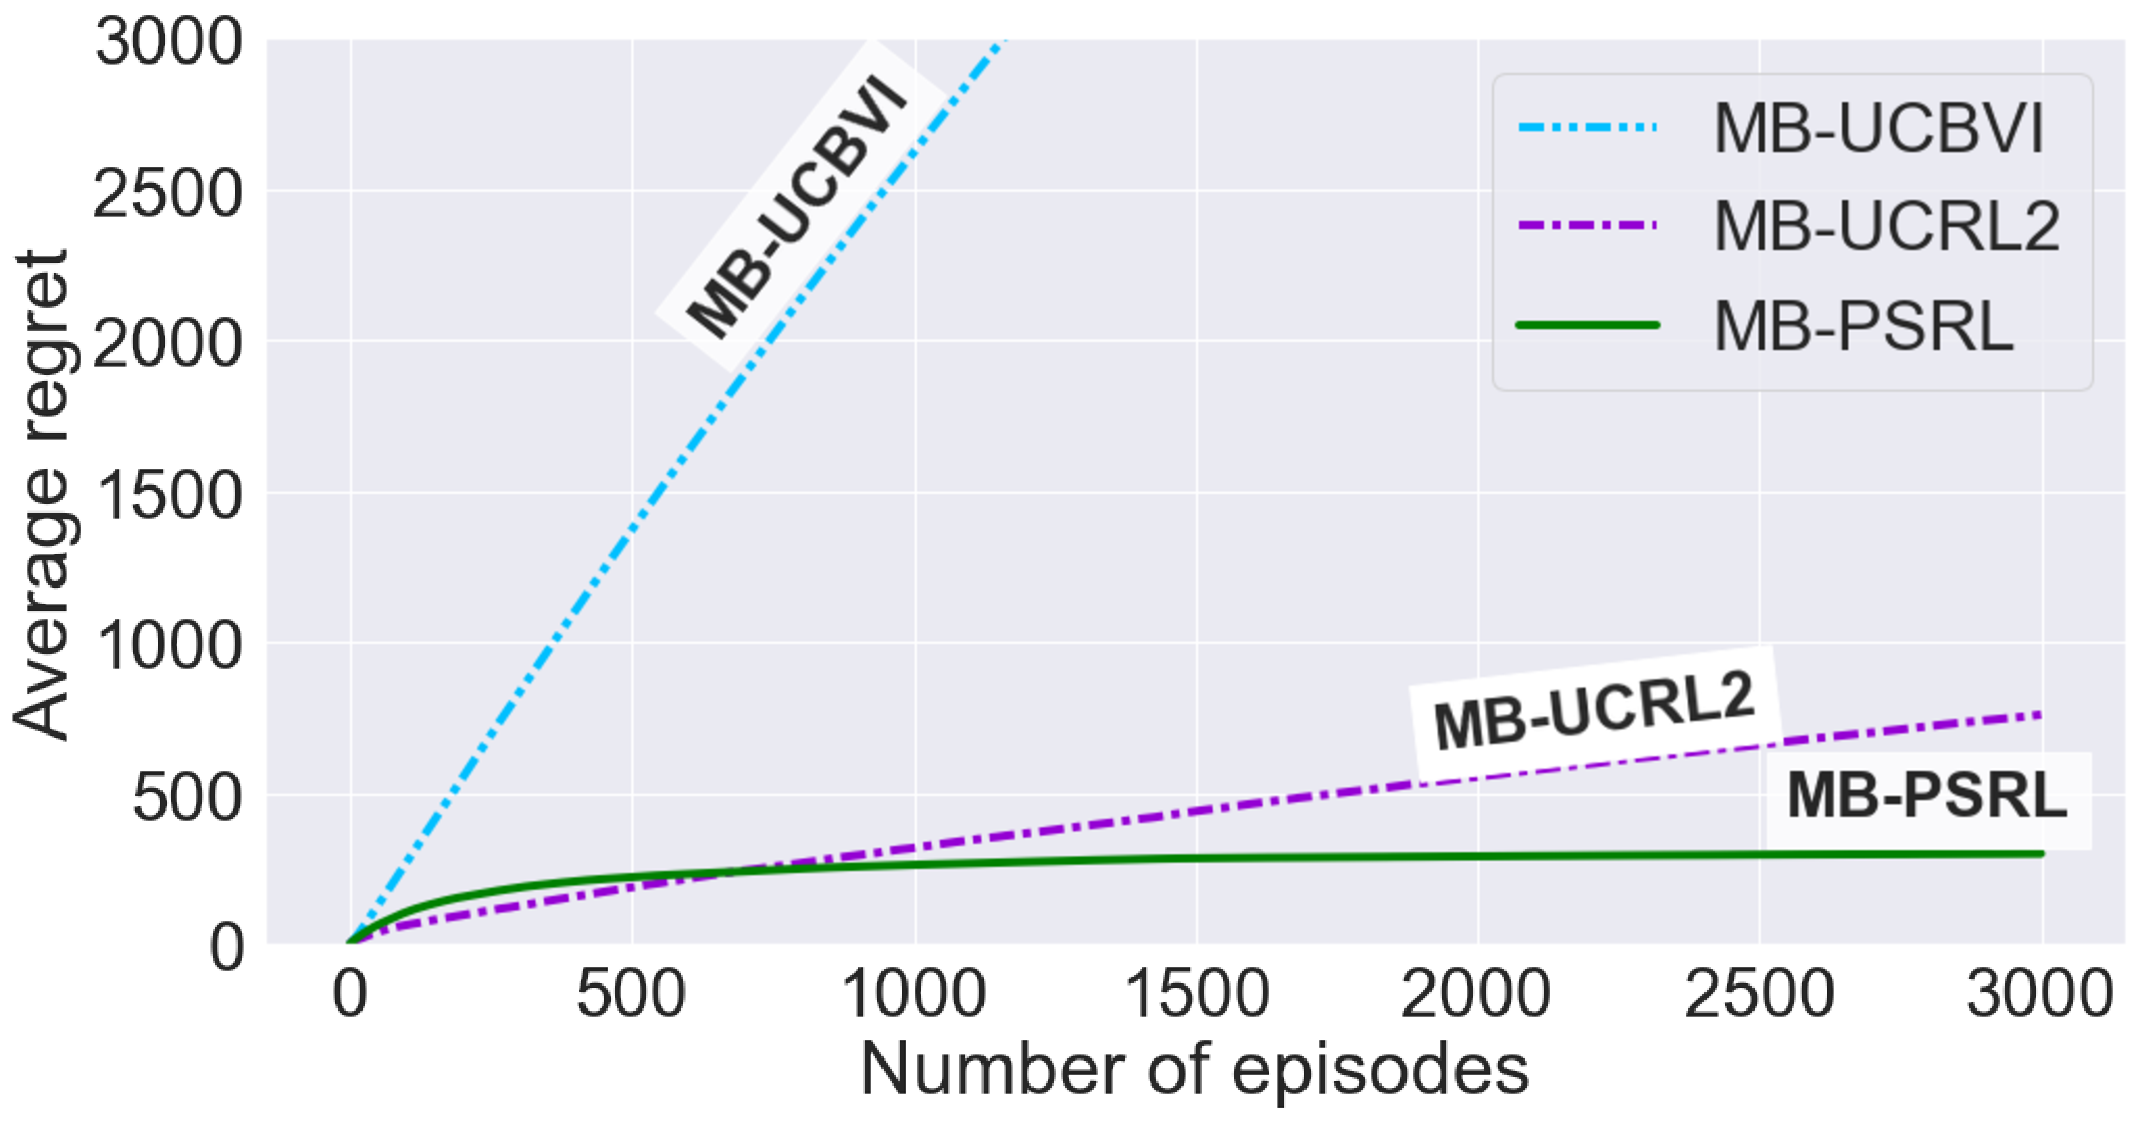
\includegraphics[width=\linewidth]{3b4s} 
            \caption{Average cumulative regret in function of the number of episodes.}
            \label{fig:randomwalk_3b4s}
        \end{subfigure}&
        \begin{subfigure}[t]{0.47\linewidth}
            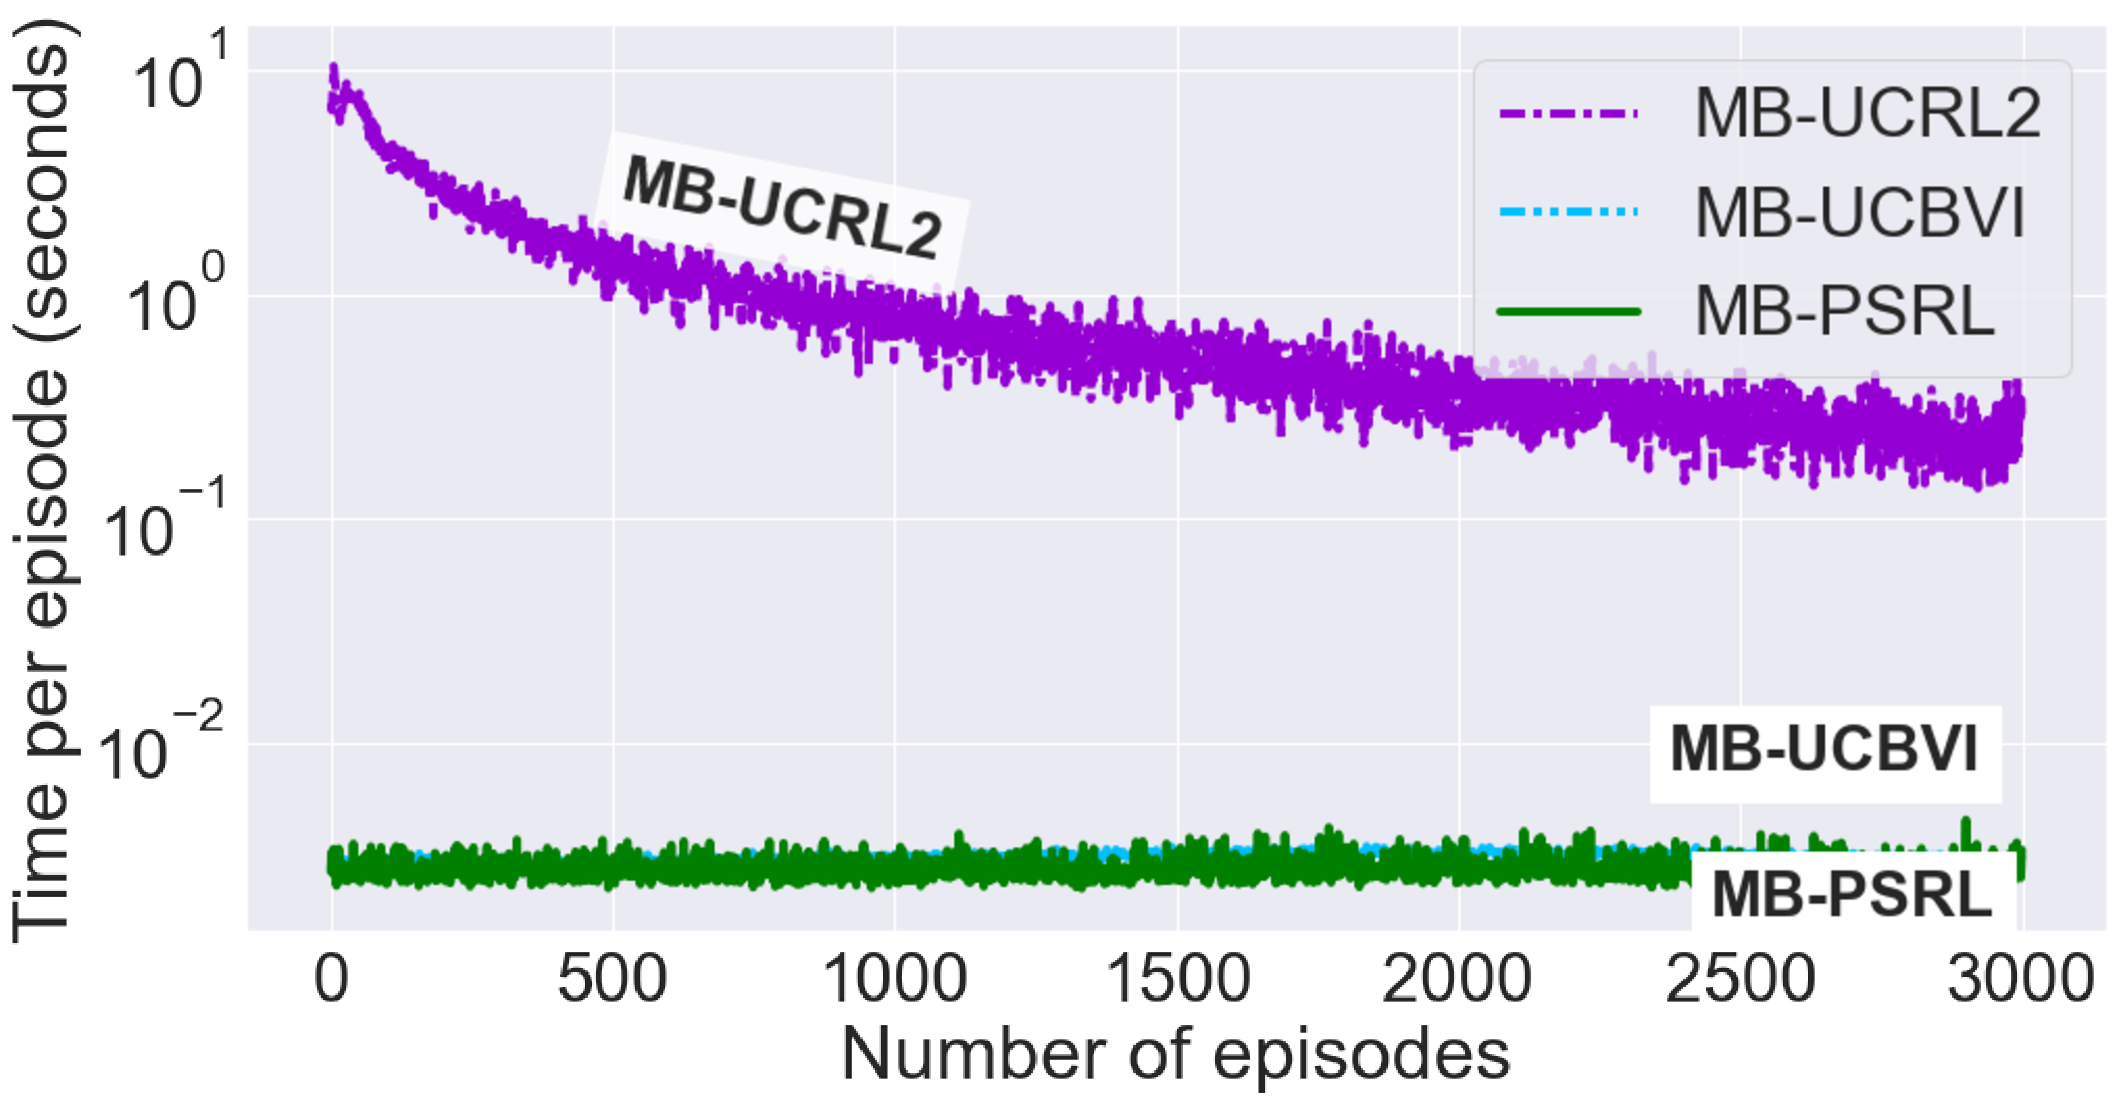
\includegraphics[width=\linewidth]{3b4s_cpt}
            \caption{Average runtime per episode. The vertical axis is in log-scale.}
            \label{fig:randomwalk_cpt_3b4s}
    \end{subfigure}
    \end{tabular}
    \caption{Experimental result for the three 4-state random walk arms given in Table~\ref{fig:randomwalk}. The $x$-axis is the number of episodes. Each algorithm is identified by a unique color for all figures.}
\end{figure}

\paragraph{Robustness (larger models and different priors)}
To test the robustness of MB-PSRL, we conduct two more sets of experiments that are reported in Appendix~\ref{apx:add_numerical}. They confirm the superiority of MB-PSRL.
The first experiment is an example from \cite{duff1995q} with $9$ arms each having $11$ states. This model illustrates the effect of the curse of dimensionality: the global  MDP has $11^9$ states which implies that the runtime of MB-UCRL2 makes it impossible to use, while MB-PSRL and MB-UCBVI take a few minutes to complete 3000 episodes.  Also in this example, MB-PSRL seems to converge faster to the optimal policy than MB-UCBVI. The second experiment tests the robustness of MB-PSRL to the choice of prior distribution. We provide numerical evidences that show that, even when MB-PSRL is run with a prior $\phi$ that is not the one from which $M$ is drawn, the regret of MB-PSRL remains acceptable (around twice the regret obtained with a correct prior). 


%%%%%%%%%%%%%%%%%%%%%%%%
%%%%%%%%%%%%%%%%%%%%%%%%
\section{Conclusion}
\label{ch:rested:sec:conclusion}

In this chapter, we present MB-PSRL, a modification of PSRL to rested Markovian bandit problems with discount. We show that its regret is close to the lower bound that we derive for this problem while its runtime scales linearly with the number of arms. Furthermore, and unlike what is usually the case, MB-PSRL does not have an optimistic counterpart that scales well: we prove that  MB-UCRL2 also has a sublinear regret but has a computational complexity exponential in the number of arms. This result generalizes to all  the variants of UCRL2 that rely on extended value iteration. We nevertheless show that OFU approach may still be pertinent for Markovian bandit problems:  MB-UCBVI, a version of UCBVI can use Gittins indices and  does not suffer from the dimensionality curse: it has a sublinear regret in terms of the number of episodes and arms as well as a linear time complexity. However, its regret bound remains larger than the one of MB-PSRL.

The broad implication of this work is that, on the one hand, if a weakly coupled MDP or factored MDP can be solved efficiently when all the parameters are known, then PSRL can be adapted to have efficient regret and runtime. On the other hand, solving weakly coupled MDP or factored MDP efficiently when all the parameters are known does not imply that all optimistic algorithms are computationally efficient. This is a major difference between the Bayesian and the optimistic approach.

\newpage

\begin{subappendices}

\begin{center}
    \bfseries \Large Appendix of the chapter
\end{center}

The section is organized as follows:
\begin{itemize}
    \item In Appendix~\ref{apx:proof_thm1}, we prove Theorem~\ref{thm:regret_upper_bound}. 
    \item In Appendix~\ref{apx:sketch_of_proof_lower}, we obtain a Bayesian minimax regret lower bound for any reinforcement learning algorithm in rested bandits (Theorem~\ref{thm:lower_bound}).
    \item In Appendix~\ref{apx:proof_OFU}, we show that \Eqref{eq:EVI} cannot be solved by local indices (Theorem~\ref{thm:no_OFU}).
    \item In Appendix~\ref{apx:algos}, we provide a detailed description of the algorithms that we use in our numerical comparisons. 
    \item In Appendix~\ref{apx:add_numerical}, we provide additional numerical experiments that show the good behavior of MB-PSRL. 
    \item In Appendix~\ref{apx:envi}, we provide details about the experimental environment and the computation time needed. 
\end{itemize}

\section{Proof of Theorem~\ref{thm:regret_upper_bound}}
\label{apx:proof_thm1}

The proof of the regret bounds for our three algorithms share a common structure but with different technical details.  In this section, we do a detailed proof of the three algorithms by factorizing as much as possible what can be factorized in the different proofs. This proof is organized as follows:
\begin{itemize}
    \item In Section~\ref{ssec:overview}, we give an overview of the proof that is common to all algorithms. 
    \item In Section~\ref{ssec:technical_lemmas}, we provide technical lemmas that are used in the detailed proofs of each algorithm. 
    \item In Section~\ref{ssec:proof_PSRL}, \ref{ssec:proof_UCRL2} and \ref{ssec:proof_UCBVI}, we provide detailed analysis of MB-PSRL, MB-UCRL2, and MB-UCBVI. 
\end{itemize}

\subsection{Overview of the Proof}
\label{ssec:overview}

Let $\pi^*$ be the optimal policy of the true MDP $M$ and $\pi^k$ the optimal policy for $M^k$, the sampled MDP at episode $k$. Recall that the expected regret is $\sum_{k=1}^K \ex{\Delta^k}$, where $\Delta^k {=} W_{M,1:H^k}^{\pi^*}(\vs_{t^k}) {-} W_{M,1:H^k}^{\pi^k}(\vs_{t^k})$.
For each of the three algorithms, we will define an event $\gE_\text{Algo}^{k}$ that is $o_{t^k}$-measurable. $\gE_\text{Algo}^{k}$ is true with high probability and guarantees that $M$ and $M^k$ are close.
We have:
\begin{align}
    \ex{\Delta^k}
    &= \ex{\Delta^k\ind{\lnot\gE_\text{Algo}^{k}} +\Delta^k\ind{\gE^{k}_\text{Algo}} } \nonumber\\
    &\le \ex{H^k}\Proba{\lnot\gE^{k}_\text{Algo}} + \ex{\Delta^k \ind{\gE^{k}_\text{Algo}}} \label{eq:gap_overview}
\end{align}
because $\Delta^k\le H^k$ and the random variables $H^k$ and $\ind{\gE^{k}_\text{Algo}}$ are independent.
For each of the three algorithms, the policy $\pi^k$ used at episode $k$ is optimal for a model $M^k$, that is either sampled from the posterior distribution for MB-PSRL, or computed by extended value iteration for MB-UCRL2, or equal to the model with the bonus for MB-UCBVI. We have
\begin{align*}
    \Delta^k=\underbrace{W_{M,1:H^k}^{\pi^*}(\vs_{t^k}) - W_{M^k,1:H^k}^{\pi^k}(\vs_{t^k})}_{:=\Delta_{model}^k}%
    + \underbrace{W_{M^k,1:H^k}^{\pi^k}(\vs_{t^k}) - W_{M,1:H^k}^{\pi^k}(\vs_{t^k})}_{:=\Delta_{conc}^k}.
\end{align*}
As we deal with the expected regret and $H^k$ is independent of the model $M^k$ and of the policy $\pi^k$, we have:
\begin{align}
    \ex{\Delta_{model}^k} = v_{M}^{\pi^*}(\vs_{t^k}) - v_{M^k}^{\pi^k}(\vs_{t^k}) \label{eq:def_model}
\end{align}
As we see later, the above equation can be used to show that $\ex{\Delta_{model}^k \ind{\gE^{k}_\text{Algo}}}$ is either $0$ (for MB-PSRL) or non-positive (for MB-UCRL2 or MB-UCBVI). 

We are then left with $\ex{\Delta_{conc}^k \ind{\gE^{k}_\text{Algo}}}$. To do so, we use Lemma~\ref{lem:regret_decomposition} to show that there exists a constant $B^k$ (equal to $H^k$ for MB-PSRL and MB-UCRL2, and $H^kL^{k}/(2(1-\gamma))$ for MB-UCBVI) such that 
\begin{align}
    &\ex{\Delta_{conc}^k\ind{\gE^{k}_\text{Algo}}}=\ex{\ind{\gE^{k}_\text{Algo}} \Big(W_{M^k,1:H^k}^{\pi^k}(\vs_{t^k}){-}W_{M,1:H^k}^{\pi^k}(\vs_{t^k})\Big)} \nonumber\\
    & {\le} \mathbb{E}\left[\ind{\gE^{k}_\text{Algo}} \sum_{t=t^k}^{t^{k+1}{-}1}\abs{r^k(s_{t,a_t}){-}r(s_{t,a_t})}{+}B^k\norm{\mP^{k}(s_{t,a_t},\cdot){-}\mP(s_{t,a_t},\cdot)}_{\ell_1}\right] \label{eq:proof2}
\end{align}
where ${\norm{\mP^{k}(s_a,\cdot)-\mP(s_a,\cdot)}_{\ell_1}=\sum_{s'_a}\abs{P^{k}(s_a,s'_a)-P(s_a,s'_a)}}$. 
For an arm $a$ and a state $s_a\in\gS_a$, we denote\footnote{In the paper, we use the notation $\ind{E}$ to denote a random variable that equals $1$ if $E$ is true and $0$ otherwise. For instance, $\ind{Y_i=y}=1$ if $Y_i=y$ and $0$ otherwise.} by $N^{k}(s_a){=} \sum_{t=1}^{t^{k}-1} \ind{s_{t,a_t}=s_a}$ the number of times that Arm~$a$ is activated before episode $k$ while being in state $s_a$. \Eqref{eq:proof2} relates the performance gap to the distance between the reward functions and transition matrices of the MDPs $M$ and $M^k$. 
With $L^K{=}\sqrt{2\ln\frac{4SnK^2\ln K}{1-\gamma}}$, the event $\gE^{k}_\text{Algo}$ guarantees that for all $a, s_a$ and $ k\ge1$, 
\begin{align}
    \label{eq:concentration}
    \abs{r^k(s_a){-}r(s_a)} {\le} \frac{L^K}{\sqrt{\max\{1,N^{k}(s_a)\}}} \text{ and }
    \norm{\mP^{k}(s_a,\cdot){-}\mP(s_a,\cdot)}_{\ell_1} {\le} \frac{2L^K {+}3\sqrt{S}}{\sqrt{\max\{1,N^{k}(s_a)\}}}
\end{align}
We use this with \Eqref{eq:proof2} to show that:
\begin{align}
    \label{eq:proof3}
    \sum_{k=1}^K\ex{\Delta_{conc}^k \ind{\gE_\text{Algo}^{k}}} &\le  \ex{C_\text{Algo}^K\sum_{k=1}^K\sum_{t=t^k}^{t^{k+1}-1}\frac{1}{\sqrt{\max\{1,N^{k}(s_a)\}}}},
\end{align}
where $C_\text{Algo}^K$ is a random variable that depends on the algorithm studied. 

The final analysis takes care of the right term of \Eqref{eq:proof3} and is more technical. It uses the fact that there cannot be too many large terms in this sum because if an arm is activated many times, then $1/\sqrt{N^{k}(s_{t,a_t})}$ is small. 
The main technical hurdle here is to deal with the $K$ random episodes $H^1,\ldots, H^K$. 
This is specific to our approach compared to the analysis of finite horizons. 
To bound this, one needs to bound terms of the form $\ex{\max_{1\leq k\leq K} (H^k)^\alpha}$ with $\alpha\in\{1.5,2\}$ (see \Eqref{eq:proof_bound}). 
To bound this, we use the geometric distribution of $H^k$ to show that $\ex{\max_{1\leq k\leq K} (H^k)^{\alpha}}=\landauO\bigl((\frac{\ln K}{1-\gamma})^{\alpha}\bigr)$ (see Lemma~\ref{lem:moment}).

\subsection{Technical lemmas common to the three algorithms}
\label{ssec:technical_lemmas}

In this section, we establish a series of lemmas that are true for any learning algorithm used. They show that:
\begin{itemize}
    \item The estimates $\hat{r}$ and $\hat{Q}$ concentrates on their true values (Lemma~\ref{lem:concentration});
    \item One can transform $\Delta_{conc}^k$ into \Eqref{eq:proof2} (Lemma~\ref{lem:regret_decomposition});
    \item The sum \Eqref{eq:proof3} can be analyzed (Lemma~\ref{lem:sum}).
\end{itemize}

\subsubsection{High Probability Events}

Recall that $o_{t^k}$ are the observations collected by the decision maker before episode $k$. Based on $o_{t^k}$, we compute the empirical estimators of reward vector and transition matrix as the following: For all $a\in[n]$ and any $s_a\in\gS_a$, let $N^{k}(s_a)=\sum_{t=1}^{t^{k}-1}\ind{s_{t,a_t}=s_a}$ be the number of times so far that an arm $a$ was activated in state $s_a$ (at episode $1$, we have ${N^1(s_a)=0}$).
Recall that $t^{k}{:=} 1 {+}\sum_{i=1}^{k-1}H^i$, and that $\hat{\vr}^{k}$ and $\hat{\mP}^{k}$ are the empirical mean reward vector and transition matrix. More precisely, $\hat{r}^{k}(s_a)$ is the empirical mean reward earned when arm $a$ is chosen while being in state $s_a$:
\begin{align*}
    \hat{r}^{k}(s_a) = \frac{1}{N^{k}(s_a)}\sum_{t=1}^{t^{k}-1} r_t\ind{a_t=a \land s_{t,a_t}=s_a},
\end{align*}
and $\hat{P}^{k}(s_a,s'_a)$ is the fraction of times that arm $a$ moved from $s_a$ to $s'_a$:
\begin{align*}
    \hat{P}^{k}(s_a,s'_a) = \frac{1}{N^{k}(s_a)}\sum_{t=1}^{t^{k}-1} \ind{a_t=a \land s_{t,a_t}=s_a \land s_{t+1,a_t}=s'_a}.
\end{align*}

We design confidence sets similar to \cite{jaksch2010near,bartlett2012regal}.

\begin{lem}
    \label{lem:concentration}
    For any $k\le K$, let $L^{k}=\sqrt{2\ln\left(2SnKk\frac{\ln(Kk)}{1-\gamma}\right)}$. Let
    \begin{align}
        \gE^{k}_H&:= \bigg\{\forall k'\le k{:} H^{k'}\le \frac{\ln(Kk)}{1-\gamma}\bigg\} \label{eq:conc_h}\\
        \gE^{k}_r&:= \bigg\{\forall a\in[n], s_a\in\gS_a, k'\le k{:} \abs{\hat{r}^{k'}(s_a){-}r(s_a)} \le \frac{L^{k}}{2\sqrt{\max\{1,N^{k'}(s_a)\}}}\bigg\} \label{eq:conc_r} \\
        \gE^{k}_P&:= \bigg\{\forall a\in[n], s_a\in\gS_a, k'\le k{:} \norm{\hat{\mP}^{k'}(s_a,\cdot){-}\mP(s_a, \cdot)}_{\ell_1} \le \frac{L^{k}{+}1.5\sqrt{S}}{\sqrt{\max\{1,N^{k'}(s_a)\}}}\bigg\} \label{eq:conc_q} \\
        \gE^{k}_v&:= \bigg\{\forall a\in[n], \vs\in\gX, k'\le k{:} \Bigl\vert\hat{r}^{k'}(s_a){-}r(s_a) \nonumber \\
                   &\quad +\gamma \sum_{\vs'\in\gX}\Bigl(\hat{p}^{k'}(\vs' \mid\vs, a) {-}p(\vs'\mid\vs,a)\Bigr)v_M^{\pi^*}(\vs')\Bigr\vert
        \le \frac{L^{k}}{2(1-\gamma)\sqrt{\max\{1,N^{k'}(s_a)\}}}\bigg\} \label{eq:conc_V}
    \end{align}
    Then, the above events are all $o_{t^k}$-measurable. Moreover:
    \begin{align*}
        &\Proba{\lnot\gE^{k}_H}\le1/K \\ 
        &\Proba{\lnot \gE^{k}_r }\le 2/K \\
        &\Proba{\lnot \gE^{k}_P }\le 2/K \\
        &\Proba{\lnot \gE^{k}_v }\le 2/K.
    \end{align*} 
\end{lem}

\begin{proof}
    For event $\gE^{k}_H$, since $\{H^{k'}\}_{k'\le k}$ are i.i.d. and geometrically distributed with parameter $(1-\gamma)$, we have that
    \begin{align*}
        \Proba{\exists k'\le k: H^{k'}>\epsilon} \le \sum_{k'=1}^{k} \Proba{H^{k'}>\epsilon} =k\gamma^{\lfloor \epsilon\rfloor}.
    \end{align*}
    Then, with $\epsilon=\frac{\ln(1/(Kk))}{\ln(\gamma)}$, we get $\Proba{\exists k'\le k: H^{k'}>\epsilon}\le 1/K$.
    Moreover,
    \begin{align*}
        \epsilon = \frac{\ln(1/(Kk))}{\ln(\gamma)}= \frac{\ln(Kk)}{\ln(1/\gamma)} < \frac{\ln(Kk)}{1-\gamma}.
    \end{align*}
    Then, $\Proba{\exists k'\le k: H^{k'}>\frac{\ln(Kk)}{1-\gamma}}\le 1/K$.

    Let $\tau^k = k\frac{\ln(Kk)}{1-\gamma}$. Under event $\gE^{k}_H$, the random variable $t^k$ is upper bounded by the deterministic quantity $\tau^k$. In what follows, we assume that event $\gE^{k}_H$ holds.

    For event $\gE^{k}_r$, let $\tilde{r}_\ell(s_a)$ be a random variable that is the empirical mean of $\ell$ i.i.d. realizations of the reward when the arm in state $s_a$ is chosen. In particular, ${\hat{r}^{k}(s_a) = \tilde{r}_{N^{k}(s_a)}(s_a)}$. By Hoeffding's inequality, for any $\epsilon>0$, one has:
    \begin{align*}
        \Proba{\abs{\tilde{r}_\ell(s_a) - r(s_a)} \ge \epsilon  } \le 2 e^{-2 \ell\epsilon^2}.
    \end{align*}
    In particular, this holds for $\epsilon=\sqrt{\frac{\ln (2SnK\tau^k)}{2\ell}}$. As $N^{k}(s_a)< \tau^k$, by using the union-bound, this implies that: 
    \begin{align}
        &\Proba{\gE^{k}_H \land \exists a, s_a, k'\le k: \abs{\hat{r}^{k'}(s_a) - r(s_a)} \ge \sqrt{\frac{\ln (2SnK\tau^k)}{2N^{k'}(s_a)}}}\label{eq:estR_k}\\
        &\qquad\le \sum_{a}\sum_{s_a}\Proba{\exists \ell\in\{1,\dots,\tau^k-1\}: \abs{\tilde{r}_{\ell}(s_a) - r(s_a)} \ge \sqrt{\frac{\ln (2SnK\tau^k)}{2\ell}}}\nonumber\\
        &\qquad\le \sum_{\ell=1}^{\tau^k}\sum_a\sum_{s_a}\Proba{\abs{\tilde{r}_{\ell}(s_a) - r(s_a)} \ge \sqrt{\frac{\ln (2SnK\tau^k)}{2\ell}}}\nonumber\\
        &\qquad\le  n S \sum_{\ell=1}^{\tau^k} 2e^{-2 \ell \frac{\ln (2SnK\tau^k)}{2\ell}} =1/K,\nonumber
    \end{align}
    where the second and third  line is the union on all possible events $N^{k'}(s_a){=}\ell$ for all ${\ell{\in}\{1,\dots, \tau^k-1\}}$.
    In total this says $\Proba{\gE^{k}_H\land \lnot \gE^{k}_r}\le 1/K$.
    Now, $\lnot \gE^{k}_r {=}(\gE^{k}_H \land \lnot \gE^{k}_r) \lor (\lnot \gE^{k}_H \land \lnot \gE^{k}_r)$.
    Then, using union bound,
    \begin{align*}
        \Proba{\lnot \gE^{k}_r}
        &\le \Proba{\lnot \gE^{k}_r \land \gE^{k}_H} + \Proba{\lnot \gE^{k}_r \land \lnot \gE^{k}_H} \\
        &\le \Proba{\lnot \gE^{k}_r \land \gE^{k}_H} + \Proba{\lnot \gE^{k}_H} \le 2/K
    \end{align*}

    The event $\gE^{k}_P$ is similar but by using Weissman's inequality \cite{weissman2003inequalities} instead of Hoeffding's bound. Indeed, by using Equation~(8) in Theorem~2.1 of \cite{weissman2003inequalities}, if $N^{k}(s_a)$ was not a random variable, one would have 
    \begin{align*}
        \Proba{\norm{\hat{\mP}^{k}(s_a,\cdot){-}\mP(s_a,\cdot)}_{\ell_1}\ge \epsilon} \le 2^S e^{- N^{k}(s_a) \epsilon^2/2}.
    \end{align*}
    Following the same approach as for \Eqref{eq:estR_k} with $\epsilon=\sqrt{2\ln(SnK\tau^k2^S)/N^{k}(s_a)}$, we use the union-bound to show that:
    \begin{align*}
        &\Proba{\gE^{k}_H\land\exists a, x_a, k'\le k: \norm{\hat{\mP}^{k'}(s_a,\cdot){-}\mP(s_a,\cdot)}_{\ell_1} {\ge} \sqrt{\frac{2\ln(SnK\tau^k 2^S)}{N^{k'}(s_a)}}} \\
        &\qquad \le \tau^k n S 2^Se^{ -N^{k'}(s_a)\frac{2\ln(SnK\tau^k2^S)}{2N^{k'}(s_a)}} = 1/K.
    \end{align*}
    By definition of $L^{k}=\sqrt{2\ln(2SnK\tau^k)}$ and since $\sqrt{x+y}\le\sqrt{x}+\sqrt{y}$, we have
    \begin{align*}
      \sqrt{2\ln(SnK\tau^k2^S)}
      &=\sqrt{2\ln(2SnK\tau^k) {+} 2(S-1)\ln 2}\\
      & \le L^{k} +\sqrt{2(S-1)\ln2} \le L^{k} + 1.5\sqrt{S}.
    \end{align*}
    Hence: 
    \begin{align*}
        &\Proba{\gE^{k}_H\land\exists a, s_a, k'\le k: \norm{\hat{\mP}^{k'}(s_a,\cdot)-\mP(s_a,\cdot)}_{\ell_1} \ge \frac{L^{k}+1.5\sqrt{S}}{\sqrt{N^{k'}(s_a)}}} \le 1/K.
    \end{align*}
    As done for $\gE_r^{k}$, we have $\lnot \gE^{k}_P {=}(\gE^{k}_H \land \lnot \gE^{k}_P) \lor (\lnot \gE^{k}_H \land \lnot \gE^{k}_P)$. With the same process, we get $\Proba{\lnot \gE^{k}_P}\le 2/K$.
        
    For event $\gE^{k}_v$, we have that $\hat{r}^{k}+\gamma\hat{p}^{k}v_M^{\pi^*}$ is the empirical mean of $r+\gamma p v_M^{\pi^*}$.
    This is because $v_M^{\pi^*}$ is deterministic and $\hat{r}^{k}$ and $\hat{p}^{k}$ are empirical mean of $r$ and $p$ respectively.
    Using Hoeffding's inequality and following the same approach above, we have $\Proba{\neg \gE^{k}_v}\le 2/K$.
\end{proof}
Note that Lemma~\ref{lem:concentration} is about the statistical properties of the observations $o_{t^k}$ in the observation space.
These properties are true for any learning algorithms.
In fact, we will combine different events of this lemma to bound the regret of our algorithm accordingly.

\subsubsection{Concentration Gap}

At episode $k$, our algorithms believe that the unknown MDP $M$ is the MDP $M^k$.
For Bayesian algorithms, $M^k$ is sampled from posterior distribution while for optimistic algorithms, $M^k$ is chosen with respect to optimism principle.
The algorithms follow the policy $\pi^k$ that is optimal for $M^k$.
Recall that $W^{\pi^k}_{M,1:H^k}(\vs)$ is the expected reward of the MDP $M$ under policy $\pi^k$, starts in state $\vs$ and lasts for $H^k$ time steps and the expected cumulative discounted reward in $M$ starting from state $\vs$ under policy $\pi^k$ is $v_{M}^{\pi^k}(\vs){=}\mathbb{E}[W^{\pi^k}_{M, 1:H^k}(\vs)]$ where $H^k\sim \mathrm{Geom}(1-\gamma)$ is the horizon of episode $k$.

\begin{lem}
    \label{lem:regret_decomposition}
    For episode $k$, let $B^k\in\R^+$ be an upper bound\footnote{We will use $B^k=H^k$ for MB-PSRL and MB-UCRL2, and $B^k=H^kL^{k}/(2(1-\gamma))$ for MB-UCBVI.} of $W_{M^k,1:H^k}^{\pi^k}(\vs)$, i.e., a constant $B^k$ such that for any $\vs\in\gX$, $W_{M^k,1:H^k}^{\pi^k}(\vs)\le B^k$. We have,
    \begin{align}
        \label{eq:lem_decompo}
        &\ex{ \Delta^k_{conc} {\mid} o_{t^k}, H^k, M^k, M} {=} \ex{ W_{M^k,1:H^k}^{\pi^k}(\vs_{t^k}){-}W_{M,1:H^k}^{\pi^k}(\vs_{t^k}) {\mid} o_{t^k}, H^k, M^k, M}\nonumber \\
        &{\le}\mathbb{E}\bigg[\sum_{t=t^k}^{t^{k+1}-1}\abs{r^k(s_{t,a_t}){-}r(s_{t,a_t})}
        {+}B^k\norm{\mP^{k}(s_{t,a_t},\cdot){-}\mP(s_{t,a_t},\cdot)}_{\ell_1} {\mid} o_{t^k}, H^k, M^k, M\bigg]
    \end{align}
\end{lem}

\begin{proof}
    From \Eqref{eq:discounted_reward} with $a=\pi^k(\vs)$,
    \begin{align}
        W^{\pi^k}_{M, 1:H^k}(\vs) 
        &=r(s_a) + \sum_{\vs'} p(\vs' \mid \vs,a)W^{\pi^k}_{M,2:H^k}(\vs'). \label{eq:decompo2}
    \end{align}
    Comparing the sampled MDP $M^k$ with the original $M$ and using \Eqref{eq:decompo2}, one has
    \begin{align}
        W^{\pi^k}_{M^k, 1:H^k}(\vs) {-} W^{\pi^k}_{M, 1:H^k}(\vs)
        &= r^k(s_a) {-} r(s_a) \nonumber \\
        &{+} \sum_{\vs'} p^k(\vs'\mid \vs,a)W^{\pi^k}_{M^k, 2:H^k}(\vs') {-} \sum_{\vs'} p(\vs' \mid \vs,a)W^{\pi^k}_{M,2:H^k}(\vs') \label{eq:depend_S}.
    \end{align}
    Note that in the above equation, the last term is of the form $p^kW^{\pi^k}_{M^k} {-}pW^{\pi^k}_{M}$, which is equal to $(p^k {-}p)W^{\pi^k}_{M^k} {+}p(W^{\pi^k}_{M^k} {-}W^{\pi^k}_{M})$. Moreover, $W_{M_k}^{\pi_k}$ is less than $B_k$.
    Plugging this to the above equation shows that:
    \begin{align*}
        &W^{\pi^k}_{M^k, 1:H^k}(\vs) {-} W^{\pi^k}_{M, 1:H^k}(\vs) \\
        &\quad\le \abs{r^k(s_a) {-} r(s_a)} {+} B^k\sum_{\vs'}\abs{p^k(\vs'\mid \vs,a) {-} p(\vs' \mid \vs,a)}\\
        &\qquad {+} \sum_{\vs'} p(\vs' \mid \vs,a)\Bigl(W^{\pi^k}_{M^k, 2:H^k}(\vs') {-} W^{\pi^k}_{M, 2:H^k}(\vs')\Bigr)\\
        &\quad {=}\abs{r^k(s_a) {-} r(s_a)} {+} B^k\norm{\vp^k(\cdot\mid \vs,a) {-} \vp(\cdot \mid \vs,a)}_{\ell_1} {+} D^{M^k,M}_{H^k}(\vs) \\
        &\qquad {+}W^{\pi^k}_{M^k, 2:H^k}(\vs_2) {-} W^{\pi^k}_{M, 2:H^k}(\vs_2)
    \end{align*}
    where $D^{M^k,M}_{H^k}(\vs){:=} \sum_{\vs'}p(\vs' \mid \vs,a)\Bigl(W^{\pi^k}_{M^k, 2:H^k}(\vs') {-} W^{\pi^k}_{M, 2:H^k}(\vs')\Bigr) {-}(W^{\pi^k}_{M^k, 2:H^k}(\vs_2) {-} W^{\pi^k}_{M, 2:H^k}(\vs_2))$.
    Note that in the equation above, $D^{M^k,M}_{H^k}(\vs)$ is a martingale difference term with ${\vs_2\sim \vp(\cdot \mid \vs,a)}$.
    Hence, the expected value of the martingale difference term is zero.
    As only arm $a$ makes a transition, we have $\norm{\vp^k(\cdot\mid \vs,a) {-} \vp(\cdot \mid \vs,a)}_{\ell_1}=\norm{\mP^{k}(s_{a},\cdot){-}\mP(s_{a},\cdot)}_{\ell_1}$. Hence, a direct induction shows that \Eqref{eq:lem_decompo} holds.
\end{proof}
\subsubsection{Bound on the double sum}

Recall that for $k\le K$, any $a\in[n]$ and any $s_a\in\gS_a$, $N^{k}(s_a)=\sum_{t=1}^{t^{k}-1}\ind{s_{t,a_t}=s_a}$ is the number of times so far that an arm $a$ was activated in state $s_a$ (at episode $1$, we have ${N^1(s_a)=0}$) and $\{H^k\}_{k\le K}$ be the sequence of episode horizons.

\begin{lem}
    For any learning algorithms, we have
    \begin{align*}
        \sum_{k=1}^K \sum_{t=t^k}^{t^{k+1}-1}\frac1{\sqrt{\max\{1,N^{k}(s_{t,a_t})\} }} \le Sn\max_{k\le K}H^k+2\sqrt{SnK\max_{k\le K}H^k}
    \end{align*}
    \label{lem:sum}
\end{lem}
\begin{proof}
Let $\tilde{N}_t(s_a)$ be the number of times that arm $a$ has been activated before time $t$ while being in state $s_a$. By definition, $\tilde{N}_{t^k}(s_a)=N^{k}(s_a)$. Moreover, if $t\in\{t^k,\dots, t^{k+1}-1\}$, then $\tilde{N}_t(s_a)\le N^{k}(s_a) + H^k$. This shows that 
\begin{align*}
    \sum_{k=1}^K \sum_{t=t^k}^{t^{k+1}-1}\frac1{\sqrt{\max\{1,N^{k}(s_{t,a_t})\} }}
    &\le \sum_{k=1}^K \sum_{t=t^k}^{t^{k+1}-1}\frac{1}{\sqrt{\max\{1, \tilde{N}_t(s_{t,a_t})-H^k\} }}\\
    &\le \sum_{t=1}^{t^{K+1}-1} \frac{1}{\sqrt{\max\{1,\tilde{N}_t(s_{t,a_t})-\max_k H^k\} }}.
\end{align*}
The above sum can be reordered to group terms by state: The above sum equals
\begin{align*}        
    \sum_{a, s_a} \sum_{m=1}^{\tilde{N}_{t^{K+1}}(s_a)} \frac{1}{\sqrt{\max\{1, m-\max_k H^k\} }}
    &\le \sum_{a, s_a} \left[\max_k H^k + \sum_{m=1}^{\max\{1,\tilde{N}_{t^{K+1}}(s_a)-\max_k H^k\}} \frac{1}{\sqrt{m}}\right],\\
    &\le Sn\max_k H^k + \sum_{a, s_a} \sum_{m=1}^{\tilde{N}_{t^{K+1}}(s_a)} \frac{1}{\sqrt{m}},\\
    &\le Sn\max_k H^k + 2\sum_{a, s_a} \sqrt{\tilde{N}_{t^{K+1}}(s_a)},
\end{align*}
where the last inequality holds because $\sum_{m=1}^{t^{K+1}}1/\sqrt{m}\le\int_1^{t^{K+1}}1/\sqrt{x}dx\le2\sqrt{{t^{K+1}}}$. 

Now, by Cauchy-Schwartz inequality, and because $\sum_{a,s_a}\tilde{N}_{t^{K{+}1}}(s_a) =t^{K{+}1}-1 {=}\sum_{k=1}^{K}H^k$, we have:
\begin{align*}
    \sum_{a,s_a}\sqrt{\tilde{N}_{t^{K+1}}(s_a)} \le \Big(\sum_{a,s_a}\tilde{N}_{t^{K+1}}(s_a)\Big)^{1/2}\Big(\sum_{a,s_a}1\Big)^{1/2}=\sqrt{Sn\sum_{k=1}^{K}H^k}\le \sqrt{SnK \max_{k\le K}H^k}.
\end{align*}
\end{proof}

\subsubsection{Bound on the expectation of $\ex{\max_{k\le K}H^k}$}

\begin{lem}
    \label{lem:moment}
    Let $\alpha\in[1,2.5]$. Then,
    \begin{align}
        \label{eq:lemma_HK}
        \ex{\max_{k\le K}(H^k)^\alpha} &\le 5+5\left(\frac{\ln K}{1-\gamma}\right)^\alpha.
    \end{align}
 \end{lem}
 \begin{proof}
    By definition, we have
    \begin{align*}
        \ex{\max_{k\le K}(H^k)^\alpha} &=  \sum_{i=1}^\infty \Proba{ \max_{k\le K}(H^k)^\alpha \ge i}\\
        &\le \sum_{i=1}^\infty \min(1, K \Proba{ (H^k)^\alpha \ge i})\\
        &= \sum_{i=1}^\infty \min(1, K \gamma^{i^{1/\alpha}}),
    \end{align*}
    where the inequality comes from the union bound, and the last equality is because the random variables $H^k$ are geometrically distributed.
 
    Let $A=\min\{i : K \gamma^{i^{1/\alpha}}\le 1\}$. Decomposing the above sum by group of size $A$, we have
    \begin{align}
        \sum_{i=1}^\infty \min(1, K \gamma^{i^{1/\alpha}})
        &= \sum_{j=0}^\infty \sum_{i=Aj+1}^{A(j+1)}\min(1, K \gamma^{i^{1/\alpha}})\nonumber\\
        &\le \sum_{j=0}^\infty A \min(1, K \gamma^{(Aj)^{1/\alpha}})\nonumber\\
        &= A + A\sum_{j=1}^\infty K (\gamma^{A^{1/\alpha}})^{j^{1/\alpha}},
        \label{eq:sum_A}
    \end{align}
    where the inequality holds because $\gamma^{i^{1/\alpha}}$ is decreasing in $i$. 
 
    By definition of $A$, we have $\gamma^{A^{1/\alpha}}\le 1/K$. This implies that the second term of \Eqref{eq:sum_A} is smaller than $\sum_{j=1}^\infty K (1/K)^{j^{1/\alpha}}=\sum_{j=1}^\infty K^{1-j^{1/\alpha}}$. As $\alpha\le 2.5$, if  $K\ge5$, this is smaller than $\sum_{j=1}^\infty 5^{1-j^{1/2.5}}\approx 3.92<4$.
 
    This shows that for $K\ge5$, we have:
    \begin{align*}
        \ex{\max_{k\le K}(H^k)^\alpha} \le 5A,
    \end{align*}
    where $A=\ceil{(-\ln K/\ln \gamma)^{\alpha}}\le 1+(\ln K/(1-\gamma ))^\alpha$.
 
    As for the case where $K\le4$, we have $\ex{\max_{k\le K}(H^k)^\alpha}\le K\ex{(H^1)^\alpha}\le \frac{K}{(1-\gamma)^{\alpha}}$. This term is smaller than \Eqref{eq:lemma_HK} for $K\le4$.
 \end{proof}


\subsection{Detailed analysis of MB-PSRL}
\label{ssec:proof_PSRL}

We decompose the analysis of PSRL in three steps: 
\begin{itemize}
    \item We define the high-probability event $\gE_\text{PSRL}^{k}$.
    \item We analyze $\sum_{k=1}^K\ex{\Delta_{model}^k \ind{\gE_\text{PSRL}^{k}}}$ (which equals $0$ here because of posterior sampling).
    \item We analyze $\sum_{k=1}^K\ex{\Delta_{conc}^k \ind{\gE_\text{PSRL}^{k}}}$. 
\end{itemize}
We will use the same proof structure for MB-UCRL2 and MB-UCBVI. 

Before doing the proof, we start by a first lemma that essentially formalizes the fact that the distribution of $M$ given $o_{t^k}$ is the same as the distribution of the sampled MDP $M^{k}$ conditioned on $o_{t^k}$. 
\begin{lem}
    \label{lem:bayesian}
    Assume that the MDP $M$ is drawn according to the prior $\phi$ and that $M^k$ is drawn according to the posterior $\phi(\cdot \mid o_{t^k})$. Then, for any $o_{t^k}$-measurable function $g$, one has:
    \begin{align}
        \label{eq:lem_bayesian}
        \ex{g(M)} = \ex{g(M^k)}. 
    \end{align}
\end{lem}
\begin{proof}
    At the start of each episode $k$, MB-PSRL computes the posterior distribution of $M$ conditioned on the observations $o_{t^k}$, and draws $M^k$ from it. This implies that $M$ and $M^k$ are identically distributed conditioned on $o_{t^k}$. Consequently, if $g$ is an $o_{t^k}$-measurable function, one has:
    \begin{align*}
        \ex{g(M) \mid o_{t^k}} = \ex{g(M^k) \mid o_{t^k}}. 
    \end{align*}
    \Eqref{eq:lem_bayesian} then follows from the tower rule. 
\end{proof}

%%%%%%%%%%%%%%
%%%%%%%%%%%%%%
\subsubsection{Definition of the high-probability event $\gE_\text{PSRL}^{k}$}

\begin{lem}
    \label{lem:concentration_psrl}
    At episode $k$, the event
    \begin{align*}
        \gE_\text{PSRL}^{k} =
        &\bigg\{ \forall a{\in}[n], s_a{\in}\gS_a, k'\le k{:}
            \abs{r^{k}(s_a){-}r(s_a)} \le\frac{L^{k}}{\sqrt{\max\{1,N^{k'}(s_a)\} }}, \\
        &\quad\norm{\mP^{k}(s_a,\cdot) {-}\mP(s_a,\cdot)}_{\ell_1} \le\frac{2L^{k}{+}3\sqrt{S}}{\sqrt{\max\{1,N^{k'}(s_a)\} }}, \text{ and } H^{k'}\le \frac{\ln(Kk)}{1-\gamma} \bigg\}
    \end{align*}
    is $o_{t^k}$-measurable and true with probability at least $1-9/K$.
\end{lem}

\begin{proof}
    Recall that for MB-PSRL, at the beginning of episode $k$, we sample an MDP $M^{k}$. We define the two events that are the analogue of the events \Eqref{eq:conc_r} and \Eqref{eq:conc_q} of Lemma~\ref{lem:concentration} but replacing the true MDP $M$ by the sampled MDP $M^{k}$: 
    \begin{align*}
        &\tilde{\gE}^{k}_r:= \bigg\{\forall a\in[n], s_a\in\gS_a, k'\le k{:} \abs{\hat{r}^{k'}(s_a){-}r^{k}(s_a)} \le \frac{L^{k}}{2\sqrt{\max\{1,N^{k'}(s_a)\} }}\bigg\} \\
        &\tilde{\gE}^{k}_P:= \bigg\{\forall a\in[n], s_a\in\gS_a, k'\le k{:} \norm{\hat{\mP}^{k'}(s_a,\cdot){-}\mP^{k}(s_a, \cdot)}_{\ell_1} \le \frac{L^{k}{+}1.5\sqrt{S}}{\sqrt{\max\{1,N^{k'}(s_a)\} }}\bigg\} 
    \end{align*}
    These events are $o_{t^k}$-measurable. Hence, Lemma~\ref{lem:bayesian}, combined with Lemma~\ref{lem:concentration} implies that $\Proba{ \lnot \tilde{\gE}^{k}_r} =\Proba{ \lnot \gE^{k}_r}\le 2/K$ and $\Proba{\lnot \tilde{\gE}^{k}_P}=\Proba{ \lnot \gE^{k}_P}\le 2/K$. Since the complement of $\gE^{k}_\text{PSRL}$ is the union of $\lnot \gE^{k}_r, \lnot \tilde{\gE}^{k}_r, \lnot \gE^{k}_P, \lnot \tilde{\gE}^{k}_P$ and $\lnot \gE^{k}_H$, the union bound implies that $\Proba{\gE_\text{PSRL}^{k}}\ge1-9/K$.
\end{proof}

\subsubsection{Analysis of $\ex{\Delta_{model}^k \ind{\gE^{k}_\text{PSRL}}}$ for MB-PSRL}

Lemma~\ref{lem:bayesian} implies that for MB-PSRL, $\ex{\Delta_{model}^k \ind{\gE^{k}_\text{PSRL}}}{=}0$ because
$\gE^{k}_\text{PSRL}$, $\pi^k$ and $M^k$ are $o_{t^k}$-measurable. 

\subsubsection{Analysis of $\ex{\Delta_{conc}^k}$ for MB-PSRL}
Following \Eqref{eq:gap_overview}, the Bayesian regret can be written as:
\begin{align}
    \BayReg(\textnormal{MB-PSRL},\phi,K)
    &= \sum_{k=1}^K \ex{\Delta^k} \le \sum_{k=1}^{K}\ex{H^k}\Proba{\neg \gE_\text{PSRL}^{k}} {+}\ex{\Delta^k \ind{\gE_\text{PSRL}^{k}}} \nonumber \\
    &\le \frac{9}{(1-\gamma)} {+} \sum_{k=1}^{K} \ex{\Delta_{model}^k\ind{\gE_\text{PSRL}^{k}}} {+} \ex{\Delta_{conc}^k\ind{\gE_\text{PSRL}^{k}}}
    \label{eq:proof_PSRL_regret}
\end{align}
where the last inequality holds due to Lemma~\ref{lem:concentration_psrl}.
By the previous section, the second term of \Eqref{eq:proof_PSRL_regret} is zero.
As all rewards are bounded by $1$, $W_{M^k,1:H^k}^{\pi^k}(\vs_{t^k})\le H^k$. Hence, by applying Lemma~\ref{lem:regret_decomposition} with the upper bound $B^k=H^k$, and because $\ind{\gE^{k}_\text{PSRL}}$ is deterministic given $o_{t^k}$, we have
\begin{align}
    \ex{\Delta^k_{conc} \ind{\gE^{k}_\text{PSRL}}}
    &= \ex{\ex{\Delta^k_{conc} \ind{\gE^{k}_\text{PSRL}} \mid o_{t^k}, H^k, M^k, M}} \nonumber \\
    &\le \mathbb{E}\bigg[ \ind{\gE^{k}_\text{PSRL}} \sum_{t=t^k}^{t^{k+1}-1}\abs{r^k(s_{t,a_t}){-}r(s_{t,a_t})} \nonumber\\
    &\qquad +H^k\norm{\mP^{k}(s_{t,a_t},\cdot){-}\mP(s_{t,a_t},\cdot)}_{\ell_1} \bigg]. \label{eq:conc_with_i}
\end{align}
Let $\gR^k := \sum_{t=t^k}^{t^{k+1}-1}\abs{r^k(s_{t,a_t}){-}r(s_{t,a_t})} {+}H^k\norm{\mP^{k}(s_{t,a_t},\cdot){-}\mP(s_{t,a_t},\cdot)}_{\ell_1}$. 
By using the definition of $\gE^{k}_\text{PSRL}$, we have:
\begin{align}
    \ind{\gE^{k}_\text{PSRL}}\gR^k 
    %&\le \ind{\gE^{k}_\text{PSRL}} \sum_{t=t^k}^{t^{k+1}-1} \frac{L^{k}{+}(2L^{k} {+}3\sqrt{S})H^k}{\sqrt{\max\{1,N^{k}(s_{t,a_t})\} }} \nonumber\\
    &\le \sum_{t=t^k}^{t^{k+1}-1} \frac{L^{k}{+}(2L^{k} {+}3\sqrt{S})H^k}{\sqrt{\max\{1,N^{k}(s_{t,a_t})\} }} \label{eq:PSRL_R_k}
\end{align}
Hence, summing over all $K$ episodes gives us:
\begin{align}
    \sum_{k=1}^{K} \ind{\gE^{k}_\text{PSRL}}\gR^k
    &\le  \big(L^K {+}(2L^K {+}3\sqrt{S})\max_{k\le K}H^k\big)\sum_{k=1}^K \sum_{t=t^k}^{t^{k+1}-1}\frac1{\sqrt{\max\{1,N^{k}(s_{t,a_t})\} }}
    \nonumber\\
    &\le  3(L^K+\sqrt{S})\max_{k\le K}H^k \sum_{k=1}^K \sum_{t=t^k}^{t^{k+1}-1}\frac1{\sqrt{\max\{1,N^{k}(s_{t,a_t})\} }},
    \label{eq:sum_not_E_k}
\end{align}
where the first inequality holds because $L^k\le L^K$ and $\max_{k\le K}H^k\ge1$. Note that the last inequality leads to a slightly worst bound but simplifies the expression. By Lemma~\ref{lem:sum}, we get
\begin{align*}
    \sum_{k=1}^{K} \ind{\gE^{k}_\text{PSRL}}\gR^k
    &\le 3(L^K+\sqrt{S})\max_{k\le K}H^k(Sn\max_{k\le K}H^k +2\sqrt{SnK \max_{k\le K}H^k}) \\
    &=3(L^K+\sqrt{S})(Sn\max_{k\le K}(H^k)^2 +2\sqrt{SnK} \max_{k\le K}(H^k)^{3/2})
    \nonumber
\end{align*}
Then, 
\begin{align}
    \sum_{k=1}^K\ex{\Delta^k_{conc} \ind{\gE^{k}_\text{PSRL}}}
    &{\le} 3(L^K {+}\sqrt{S})\bigg(Sn\ex{\max_{k\le K}(H^k)^2} {+}2\sqrt{SnK} \ex{\max_{k\le K}(H^k)^{3/2}}\bigg) \label{eq:proof_bound}\\
    &{\le} 3(L^K {+}\sqrt{S})\bigg(Sn\Bigl(5 {+}5\Bigl(\frac{\ln K}{1-\gamma}\Bigr)\Bigr)^2 {+}\sqrt{SnK}\Bigl(5 {+}5\Bigl(\frac{\ln K}{1-\gamma}\Bigr)\Bigr)^{3/2}\bigg) \nonumber
\end{align}
where the last inequality is true due to Lemma~\ref{lem:moment}.
With $L^K{=}\sqrt{2\ln\Bigl(2SnK^2\frac{\ln K^2}{1-\gamma}\Bigr)}$, this implies that there exists a constant $C$ independent of all problem's parameters such that:
\begin{align*}
    \BayReg(\textnormal{MB-PSRL},\phi,K) {\le} C\Bigl(\sqrt{S}{+}\ln \frac{SnK\ln K}{1-\gamma}\Bigr) \left(Sn\Bigl(\frac{\ln K}{1-\gamma}\Bigr)^{2}
    {+}\sqrt{SnK}\Bigl(\frac{\ln K}{1-\gamma}\Bigr)^{3/2}\right).
\end{align*}

\subsubsection{Remark on the dependence on $S$}
\label{sssec:psrl_s}

Our bound is linear in $S$, the state size of each arm, because our proof follows the approach used in \cite{osband2013more}. Using another proof methodology, it is argued in \cite{osband2017posterior} that the regret of PSRL grows as the square root of the state space size and not linearly. In our paper, we choose to use the more conservative approach of \cite{osband2013more} because we believe that the proof used in \cite{osband2017posterior} is not correct (in particular the use of a deterministic $v$ in Equation~(16) of the proof of Lemma~3 in Appendix~A in the arXiv version of \cite{osband2017posterior} seems incompatible with the use of Lemma~4 of the same paper).
In fact, when considering the worst case realization of $v$, the concentration bound in Equation~(16) of the paper is equivalent to the (scaled) L1 norm of transition concentration.
We are not alone to point out this error. Effectively, \cite{agrawal2017posterior} used Lemma~C.1 and Lemma~C.3 (equivalence of Lemma~3 of \cite{osband2017posterior}) to get a bound in square root of the state space size. But both lemmas are erroneous as mentioned in the latest arXiv version of \cite{agrawal2017posterior}. The validity of Lemma~3 is also questioned on page 87 of \cite{fruit2019exploration}. While it is informal, the recent work of \cite{qian2020concentration} also theoretically contradicts the lemma.

\subsection{Case of MB-UCRL2}
\label{ssec:proof_UCRL2}

The proof follows the same steps as for MB-PSRL. While the high probability event is simpler, the additional complication is to show that $\sum_{k=1}^K\ex{\Delta_{model}^k}\le0$ by using the optimism principle. 

\subsubsection{Definition of the high probability event} 

\begin{lem}
    \label{lem:concentration_ucrl}
    At episode $k$, the event
    \begin{align*}
        \gE_\text{UCRL2}^{k} =
        &\bigg\{ \forall a{\in}[n], s_a{\in}\gS_a, k'\le k{:}
            \abs{\rhat^{k'}(s_a){-}r(s_a)} \le\frac{L^{k}}{2\sqrt{\max\{1,N^{k'}(s_a)\} }}, \\
        &\quad\norm{\hat{\mP}^{k'}(s_a,\cdot) {-}\mP(s_a,\cdot)}_{\ell_1} \le\frac{L^{k}{+}1.5\sqrt{S}}{\sqrt{\max\{1,N^{k'}(s_a)\} }}, \text{ and } H^{k'}\le \frac{\ln(Kk)}{1-\gamma} \bigg\}
    \end{align*}
    is $o_{t^k}$-measurable and true with probability at least $1-5/K$.
\end{lem}
\begin{proof}
    The complement of $\gE^{k}_\text{UCRL2}$ is the union of $\neg \gE^{k}_r, \neg \gE^{k}_P$ and $\neg \gE^{k}_H$. We conclude the proof by using the union bound and $\Proba{\neg \gE^{k}_r} \le 2/K$, $\Proba{\neg \gE^{k}_P} \le 2/K$ and $\Proba{\neg \gE^{k}_H} \le 1/K$. 
\end{proof}

\subsubsection{Analysis of $\ex{\Delta_{model}^k\ind{\gE^{k}_\text{UCRL2}}}$ -- Optimism of MB-UCRL2}

Recall that $\pi^*$ is the optimal policy of the unknown MDP $M$ and that $\pi^k$ is the policy used in episode $k$. $\pi^k$ is optimal for the optimistic MDP that is chosen from the plausible MDP set $\sM^k$:
\begin{align*}
    \pi^k \in \argmax_{\pi} \max_{M'\in\sM^k} v^\pi_{M'}.
\end{align*}
For each episode $k$, the plausible MDP set $\sM^k$ is defined by
\begin{align}
    \label{eq:plausible}
    \sM^k=\bigg\{(\vr',\mP'):\forall a, s_a, \abs{r'(x_a)-\hat{r}^{k}(s_a)} \le \frac{L^{k}}{2\sqrt{\max\{1,N^{k}(s_a)\} }} \text{, and }\nonumber\\
    \norm{\mP'(s_a,\cdot)-\hat{\mP}^{k}(s_a, .)}_{\ell_1} \le \frac{L^{k}+1.5\sqrt{S}}{\sqrt{\max\{1,N^{k}(s_a)\} }}\bigg\}.
\end{align}
As \cite{jaksch2010near}, we argue that there exists an MDP $M^k\in\sM^k$ such that $\pi^k$ is an optimal policy for $M^k$. Moreover, under event $\gE_\text{UCRL2}^{k}$, one has $M\in \sM^k$, which implies that $\max_{\pi}\max_{M'\in \sM^k} v^{\pi}_{M'}(\vs)\ge v^{\pi^*}_M(\vs)$. By \Eqref{eq:def_model}, we get $\ex{\Delta_{model}^k}{\le} 0$.
If $\gE_\text{UCRL2}^{k}$ does not hold, we simply have $\Delta_{model}^k\ind{\gE^{k}_\text{UCRL2}}=0$. We conclude that: $\ex{\Delta_{model}^k\ind{\gE_\text{UCRL2}^{k}}}{\le}0$. 


\subsubsection{Analysis of $\ex{\Delta_{conc}^k\ind{\gE_\text{UCRL2}^{k}}}$ for MB-UCRL2}
Following \Eqref{eq:gap_overview}, the expected regret can be written as:
\begin{align}
    \ex{\Reg(\text{MB-UCRL2},M,K)}
    &= \sum_{k=1}^K \ex{\Delta^k} \le \sum_{k=1}^{K}\ex{H^k}\Proba{\neg \gE_\text{UCRL2}^{k}} {+}\ex{\Delta^k \ind{\gE_\text{UCRL2}^{k}}} \nonumber \\
    &\le \frac{5}{1-\gamma} {+} \sum_{k=1}^{K} \ex{\Delta_{model}^k\ind{\lnot\gE_\text{UCRL2}^{k}}} {+} \ex{\Delta_{conc}^k\ind{\lnot\gE_\text{UCRL2}^{k}}}
    \label{eq:proof_UCRL2_regret}
\end{align}
where the last inequality holds due to Lemma~\ref{lem:concentration_ucrl}.
By the previous section, the second term of \Eqref{eq:proof_UCRL2_regret} is non-positive.
In the following, we therefore analyze the last term whose analysis is then similar to the one for MB-PSRL.  Indeed, with $B^k=H^k$ and definition of $\gE^{k}_\text{UCRL2}$, the use of Lemma~\ref{lem:regret_decomposition} shows that one has
\begin{align*}
    \ex{\Delta_{conc}^k\ind{\gE^{k}_\text{UCRL2}}} \le \ex{\frac12 \sum_{t=t^k}^{t^{k+1}-1}\frac{L^{k} {+}(2L^{k} {+} 3\sqrt{S}) H^k}{\sqrt{\max\{1,N^{k}(s_{t,a_t})\} }}}.
\end{align*}
Up to a factor $1/2$, the expression inside the expectation is the same as \Eqref{eq:PSRL_R_k} of MB-PSRL. Hence, one can use Lemma~\ref{lem:sum} the same way to show that
\begin{align*}
    \sum_{k=1}^{K} \ex{\Delta^k_{conc}\ind{\gE^{k}_\text{UCRL2}}}
    \le \frac32(L^K+\sqrt{S})\bigg(Sn\ex{\max_{k\le K}(H^k)^2} +2\sqrt{SnK} \ex{\max_{k\le K}(H^k)^{3/2}}\bigg).
\end{align*}
Up to a factor $1/2$, the right term of the above equation is equal to the right term of \Eqref{eq:proof_bound}. Following the same process done for the latter, we can conclude that there exists a constant $C'$ independent of all problem's parameters such that:
\begin{align*}
    \Reg(\text{MB-UCRL2},M,K) \le C'\Bigl(\sqrt{S}{+}\ln \frac{SnK\ln K}{1-\gamma}\Bigr) \left(Sn\Bigl(\frac{\ln K}{1-\gamma}\Bigr)^{2}
    {+}\sqrt{SnK}\Bigl(\frac{\ln K}{1-\gamma}\Bigr)^{3/2}\right).
\end{align*}


\subsection{Case of MB-UCBVI}
\label{ssec:proof_UCBVI}

We start by defining the high probability event. Then, we prove the optimistic property of MB-UCBVI. Finally, we bound its expected regret.

\subsubsection{Definition of the high-probability event}

\begin{lem}
    \label{lem:concentration_ucbvi}
    The event
    \begin{align*}
        &\gE_\text{UCBVI}^{k} {=}\bigg\{ \forall a{\in}[n], \vs{\in}\gX, k'\le k{:} \\
        &\qquad \abs{\rhat^{k'}(s_a){-}r(s_a)} \le\frac{L^{k}}{2\sqrt{\max\{1,N^{k'}(s_a)\} }}, \\
        &\qquad \norm{\hat{\mP}^{k'}(s_a,\cdot) {-}\mP(s_a,\cdot)}_{\ell_1} \le\frac{L^{k}{+}1.5\sqrt{S}}{\sqrt{\max\{1,N^{k'}(s_a)\} }}, H^{k'}\le \frac{\ln(Kk)}{1-\gamma}, \text{ and } \\
        &\abs{\rhat^{k'}(s_a){-}r(s_a) {+}\gamma\sum_{\vs'}(\hat{p}^{k'}(\vs'\mid\vs,a){-}p(\vs'\mid\vs,a))v_M^{\pi^*}(\vs')} \le
    \frac{L^{k}}{2(1{-}\gamma)\sqrt{\max\{1,N^{k'}(s_a)\} }} \\
        &\bigg\}
    \end{align*}
    is $o_{t^k}$-measurable and true with probability at least $1-7/K$.
\end{lem}
\begin{proof}
    The complement of $\gE^{k}_\text{UCBVI}$ is the union of $\neg \gE^{k}_r, \neg \gE^{k}_P, \neg \gE^{k}_H$ and $\neg \gE^{k}_v$.
    We conclude the proof by using the union bound and $\Proba{\neg \gE^{k}_r} \le 2/K$, $\Proba{\neg \gE^{k}_P} \le 2/K$, $\Proba{\neg \gE^{k}_H} \le 1/K$, and $\Proba{\neg \gE^{k}_v} \le 2/K$.
\end{proof}

\subsubsection{Analysis of $\ex{\Delta_{model}^k \ind{\gE^{k}_\text{UCBVI}}}$ -- Optimism of MB-UCBVI}

The following lemma guarantees that $\ex{\Delta_{model}^k \ind{\gE^{k}_\text{UCBVI}}}\le0$. Indeed, as $\gE^{k}_\text{UCBVI}$ is $o_{t^k}$-measurable, one has 
\begin{align*}
    \ex{\Delta_{model}^k\ind{\gE^{k}_\text{UCBVI}}} &= \ex{\ex{\Delta_{model}^k\mid o_{t^k}}\ind{\gE^{k}_\text{UCBVI}}}\\
    &=\ex{(v_M^{\pi^*}(\vs_{t^k}) - v_{M^k}^{\pi^k}(\vs_{t^k}))\ind{\gE^{k}_\text{UCBVI}}} \le 0.
\end{align*}
\begin{lem}
    \label{lem:ucbvi_optim}
   If $\gE^{k}_\text{UCBVI}$ holds, then for any $\vs\in\gX$, we have
   \begin{align*}
       v_{M^k}^{\pi^k}(\vs) \ge v_{M}^{\pi^*}(\vs)
    \end{align*}
\end{lem}
\begin{proof}
    Recall that at episode $k$, we define the optimistic MDP of MB-UCBVI by $M^k$ in which the parameters of any arm $a\in[n]$ are $(\hat{\vr}^{k}_a +\beta^{k}_r, \hat{\mP}^{k}_a)$ with $\beta^k(s_a){=}\frac{L^{k}}{2(1-\gamma)\sqrt{\max\{1,N^{k}(s_a)\} }}$ for any $s_a\in\gS_a$.
The Gittins index policy $\pi^k$ is optimal for MDP $M^k$.
For any state $\vs$, let $a=\pi^k(\vs)$ and $a^*=\pi^*(\vs)$.
Then,
\begin{align*}
    v_{M^k}^{\pi^k}(\vs) -v_M^{\pi^*}(\vs)
    &= \beta^k_r(s_a) +\rhat^{k}(s_a) +\gamma\sum_{\vs'}\hat{p}^{k}(\vs'\mid \vs,a)v_{M^k}^{\pi^k}(\vs') -v_M^{\pi^*}(\vs)\\ 
    &\ge \beta^{k}_r(s_{a^*}) +\rhat^{k}(s_{a^*}) +\gamma\sum_{\vs'}\hat{p}^{k}(\vs'\mid \vs,a^*)v_{M^k}^{\pi^k}(\vs') \\
    &\quad -r(s_{a^*}) -\gamma\sum_{\vs'}p(\vs'\mid \vs,a^*)v_M^{\pi^*}(\vs') \\
    &= \beta^{k}_r(s_{a^*}) +\rhat^{k}(s_{a^*}) {-}r(s_{a^*}) {+}\gamma\sum_{\vs'}\Bigl(\hat{p}^{k}(\vs'\mid \vs,a^*) {-}p(\vs'\mid \vs,a^*)\Bigr)v_M^{\pi^*}(\vs') \\
    &\qquad +\gamma \sum_{\vs'}\hat{p}^{k}(\vs'\mid \vs,a^*)\Bigl(v_{M^k}^{\pi^k}(\vs') -v_M^{\pi^*}(\vs')\Bigr)
\end{align*}
Let $(r^{\pi}, P^{\pi})$ be the reward vector and transition matrix under policy $\pi$ (i.e. $\forall \vs, \vs'\in\gX, r^{\pi}(\vs)=r(s_{\pi(\vs)}), P^{\pi}(\vs,\vs')=p\Bigl( \vs'\mid \vs,\pi(\vs)\Bigr)$ as defined in \Eqref{eq:defP}).
In matrix form, the above equations
\begin{align*}
    v_{M^k}^{\pi^k} -v_M^{\pi^*}
    &\ge (\beta_r^{k})^{\pi^*} +(\rhat^{k})^{\pi^*} -r^{\pi^*} {+}\gamma\Bigl((\Phat^{k})^{\pi^*} {-}P^{\pi^*}\Bigr)v_M^{\pi^*} +\gamma (\Phat^{k})^{\pi^*}(v_{M^k}^{\pi^k} -v_M^{\pi^*}).
\end{align*}
Under event $\gE^{k}_\text{UCBVI}$, $(\beta_r^{k})^{\pi^*} +(\rhat^{k})^{\pi^*} -r^{\pi^*} {+}\gamma\Bigl((\Phat^{k})^{\pi^*} {-}P^{\pi^*}\Bigr)v_M^{\pi^*}\ge 0$. This implies that:
\begin{align*}
    \Bigl(I-\gamma (\Phat^{k})^{\pi^*}\Bigr)(v_{M^k}^{\pi^k} -v_M^{\pi^*}) &\ge 0.
\end{align*}
As $\Bigl(I-\gamma (\Phat^{k})^{\pi^*}\Bigr)^{-1} = I+ \Bigl(I-\gamma (\Phat^{k})^{\pi^*}\Bigr) +\Bigl(I-\gamma (\Phat^{k})^{\pi^*}\Bigr)^2 +\dots$ is a matrix whose coefficients are all non-negative, this implies that $v_{M^k}^{\pi^k} -v_M^{\pi^*} \ge 0$. 
\end{proof}

\subsubsection{Analysis of $\ex{\Delta_{conc}^k\ind{\gE_\text{UCBVI}^{k}}}$ for MB-UCBVI}
Following \Eqref{eq:gap_overview}, the expected regret can be written similarly to \Eqref{eq:proof_UCRL2_regret} for MB-UCRL2, one can write that
\begin{align*}
    \ex{\Reg(\text{MB-UCBVI},M,K)}
    &\le \frac{7}{1-\gamma} {+} \sum_{k=1}^{K} \ex{\Delta_{model}^k\ind{\gE_\text{UCBVI}^{k}}} {+} \ex{\Delta_{conc}^k\ind{\gE_\text{UCBVI}^{k}}}.
\end{align*}
The same as MB-UCRL2, the second term is non-positive.
We are therefore left with the last term.
Using Lemma~\ref{lem:regret_decomposition} with $B^k=\frac{H^kL^{k}}{2(1-\gamma)}$ and the definition of $M^k$ for MB-UCBVI, we have:
\begin{align*}
    \sum_{k=1}^K \ex{ \ind{\gE^{k}_\text{UCBVI}} \Delta^k_\text{conc}}
    &{\le} \sum_{k=1}^K \mathbb{E}\bigg[ \ind{\gE^{k}_\text{UCBVI}}\sum_{t=t^k}^{t^{k+1}-1} \beta^{k}_r(s_{t,a_t}){+}\abs{\rhat^{k}(s_{t,a_t}){-}r(s_{t,a_t})} \\
    &\qquad {+}\frac{H^kL^{k}}{2(1-\gamma)}\norm{\hat{\mP}^{k}(s_{t,a_t},\cdot){-}\mP(s_{t,a_t},\cdot)}_{\ell_1} \bigg] \\
    &\le \ex{\sum_{k=1}^{K}\sum_{t=t^k}^{t^{k+1}-1} \frac{(2-\gamma)L^{k}+H^kL^{k}(L^{k}+1.5\sqrt{S})}{2(1-\gamma)\sqrt{\max\{1,N^{k}(s_{t,a_t})\} }}} \\
    &\le \ex{\frac{2L^K(L^K+\sqrt{S})\max_{k\le K}H^k}{1-\gamma} \sum_{k=1}^{K} \sum_{t=t^k}^{t^{k+1}-1} \frac1{\sqrt{\max\{1,N^{k}(s_{t,a_t})\} }}} \\
    &\le \ex{\frac{2L^K(L^K+\sqrt{S})\max_{k\le K}H^k}{1-\gamma} \p{Sn\max_{k\le K}H^k +2\sqrt{SnK\max_{k\le K}H^k} }} 
\end{align*}
where the second inequality holds due to the definition of $\gE^{k}_\text{UCBVI}$ and the last one holds due to Lemma~\ref{lem:sum}.
With $L^K{=}\sqrt{2\ln\Bigl(\frac{2SnK^2\ln K^2}{1-\gamma}\Bigr)}$, we have
\begin{align*}
    \sum_{k=1}^K \ex{ \ind{\gE^{k}_\text{UCBVI}} \Delta^k_{conc}}
    &\le \frac{4(1{+}\sqrt{S})}{1-\gamma} \ln \Bigl(\frac{4SnK^2\ln K}{1-\gamma}\Bigr) \Bigl(Sn\ex{\max_{k\le K}(H^k)^2} \\
    &\qquad {+}2\sqrt{SnK} \ex{\max_{k\le K}(H^k)^{3/2}}\Bigr)
\end{align*}
The last term of the right side above can be analyzed exactly the same as what is done for \Eqref{eq:proof_bound} using Lemma~\ref{lem:moment}.
This concludes the proof.

\subsubsection{Remark on the dependence on $S$}
\label{sssec:ucbvi_s}

In the analysis of UCBVI and in our analysis, one need to bound the last term of \Eqref{eq:depend_S}
which is of the form ${\vp^kW^{\pi^k}_{M^k} -\vp W^{\pi^k}_{M}}$. \cite{azar2017minimax} rewrite this term as
$(\vp^k -\vp)W^{\pi^*}_M +(\vp^k -\vp)(W^{\pi^k}_{M^k} -W^{\pi^*}_M) +\vp(W^{\pi^k}_{M^k} {-}W^{\pi^k}_{M})$.
They then bound the first term by Chernoff-Hoeffding's inequality because the optimal value of the unknown MDP is deterministic.
The second term, called the "correction" term, is bounded by using Bernstein's inequality and the optimism \cite[Step 1, page 6]{azar2017minimax}. The third term is bounded by using the inequalities for martingale difference sequences. This allows the authors to have a factor $\sqrt{S}$ (instead of the classical $S$) in the regret bound.

If the technique to deal with the first and third terms would also apply to our case, the analysis of the second term uses heavily the optimism and the fact that $W^{\pi^k}_{M^k}\ge W^{\pi^*}_{M}$ in their setting. This cannot be adapted for MB-UCBVI because the optimism implies that $v^{\pi^k}_{M^k} \ge v^{\pi^*}_{M}$ but we do not necessarily have $W^{\pi^k}_{M^k,h:H^k}(\vs')\ge W^{\pi^*}_{M,h:H^k}(\vs')$ for all $\vs'\in\gX$, all $h\in[H^k]$ and all $k$. This is because we might lose the optimism when working with the value function over random episode length.
That is why we need to use Lemma~\ref{lem:regret_decomposition} which is more conservative.

%%%%%%%%%%%
%%%%%%%%%%%
\section{Proof of Theorem~\ref{thm:lower_bound}}
\label{apx:sketch_of_proof_lower}

To prove the lower bound, we consider a specific Markovian bandit problem that is composed of $S$ independent \emph{stochastic bandit problems}. 
This allows us to reuse the existing minimax lower bound for stochastic bandit problems. 
This existing result can be stated as follows: let $\gL\sto$ be a learning algorithm for the stochastic bandit problem. 
It is shown in Theorem~3.1 of \cite{bubeck2012regret} that for any number of arms $n$ and any number of time steps $\tau$, there exists parameters for a stochastic bandit problem $M\sto$ with $n$ arms such that the regret of the learning algorithm over $\tau$ time steps is at least $(1/20)\sqrt{n \tau}$. 
\begin{align}
    \label{eq:regret_sto}
    \Reg\sto( \tau, \gL\sto, M\sto) \ge \frac1{20}\sqrt{n\tau}. 
\end{align}
This lower bound (Theorem~3.1 of \cite{bubeck2012regret}) is constructed by considering $n$ stochastic bandit problems $M\stoi$ for $j\in[n]$ with parameters that depend on $\tau$ and $n$. 
In the problem $M\stoi$, all arms have a reward $\theta(\tau,n)$ except arm $j$ that has a reward $\theta'(\tau,n)>\theta(\tau,n)$. 
It is shown in Theorem~3.1 of \cite{bubeck2012regret} that a learning algorithm cannot perform uniformly well on all problems because it is impossible to distinguish them \emph{a priori}. 
More precisely, in the proof of Lemma~3.2 of \cite{bubeck2012regret}, it is shown that if the best arm is chosen at random, then the expected (Bayesian) regret of any learning algorithm is at least $(1/20)\sqrt{n \tau}$.

As for our problem, let $K$ be a number of episodes, $\gamma$ a discount factor, $n$ a number of arms, $S$ a number of states per arm and set $\tau=K/(2S(1-\gamma))$. 
We consider a random Markovian bandit model $M$ constructed as follows. 
Each arm $a$ has $S$ states with the state space $\gS_a = \{ 1_a,2_a,\ldots, S_a\}$. 
The transition matrix $\mP_a$ is the identity matrix. 
For each state $i\in\{1,\dots, S\}$, we choose the best arm $a^*_i$ uniformly at random among the $n$ arms, independently for each $i$. 
The rewards of a state $i_a$ are \emph{i.i.d.} Bernoulli rewards with mean $\theta(\tau,n)$ if $a\ne a^*_i$ and $\theta'(\tau,n)$ if $a=a^*_i$. 
The initial distribution $\rho$ couples the initial states of all arms for all $i\in\{1,\dots, S\}$, 
\begin{align*}
    \Proba{\forall a\in[n]: s_{1,a} = i_a} = \frac1S. 
\end{align*} 
In this case, the Markovian bandit problem becomes a combination of $S$ independent stochastic bandit problems with $n$ arms each. 
We denote by $M\sto_i$ the random stochastic bandit problem for the initial state $\vi=(i_a)_{a\in[n]}$. As the best arm $a^*_i$ are chosen independently for each $i$, a learning algorithm $\gL$ cannot use the information from $M\sto_i$ to perform better on $M\sto_j$, $j\ne i$.

Let $\phi$ be the distribution of the random Markovian bandit model $M$ defined above and let $T_i$ be the number of time steps spent in state $\vi$ by the learning algorithm $\gL$.
\begin{align}
    \BayReg(\gL, \phi, K)
    &\ge \sum_{i=1}^S\ex{\Reg\sto(T_i, \gL\sto_i, M\sto_i)} \nonumber\\
    &\ge \sum_{i=1}^S\ex{\Reg\sto(\tau, \gL\sto_i,  M\sto_i)\ind{T_i\ge\tau}}\label{eq:non-decreasing}\\
    &\ge \frac{S}{20} \sqrt{n\tau}\Proba{T_i\ge \tau}\label{eq:lower2}\\
    &= \frac1{20} \sqrt{\frac{SnK}{2(1-\gamma)}}\Proba{T_i\ge \tau},\label{eq:tau}
\end{align}
where \Eqref{eq:non-decreasing} is true because the expected regret is non-decreasing function of the number of episodes, \Eqref{eq:lower2} comes from \Eqref{eq:regret_sto} and \Eqref{eq:tau} from the definition of $\tau$.

We show in the Lemma~\ref{lem:concentration_T_i} below that $\Proba{T_i\le K/(2S(1-\beta))}\le 8S/K$. This shows that for $K\ge16S$, one has $\Proba{T_i\ge \tau}\ge1/2$. This concludes the proof as $40\sqrt{2}\le60$. 

\begin{lem}
    \label{lem:concentration_T_i}
    Recall that $T_i$ is the number of time steps that the MDP is in state $\vi$ for the MDP model above. Let $G_k$ be a sequence of \emph{i.i.d.} Bernoulli random variable of mean $1/S$ and let $H_k$ be an independent \emph{i.i.d.} sequence of geometric random variable of parameter $1-\beta$. Then:
    \begin{itemize}
        \item[(i)] $T_i\sim\sum_{k=1}^K G_k H_k$,
        \item[(ii)] $\ex{T_i} = K/(S(1-\beta))$,
        \item[(iii)] $\Proba{T_i \ge \ex{T_i}/2} \ge 1-8S/K$. 
    \end{itemize}
\end{lem}
\begin{proof}
    Let $G_k$ be a random variable that equals $1$ if the initial state $\vi$ is chosen at the beginning of episode $k$ and recall that $H_k$ is the episode length. By definition, the variables $G_k$ and $H_k$ are independent and follow respectively Bernoulli and geometric distribution. This shows \emph{(i)}. 
    
    Let $W_k=G_kH_k$. As the $W_k$ are \emph{i.i.d.} and $G_k$ and $H_k$ are independent, we have: 
    \begin{align*}
        \ex{T_i} = K\ex{H_1G_1} &= \frac{K}{S(1-\beta)}.
    \end{align*}
    This shows (ii). 
    
    Moreover, $\var{T_i} = K\var{H_1G_1}$. Hence, by using Chebyshev's inequality, one has:
    \begin{align*}
        \Proba{T_i \le \frac{\ex{T_i}}{2}} &\le \Proba{\norm{T_i-\ex{T_i}} \ge \frac{\ex{T_i}}{2}}\\
        &\le \frac{4\var{T_i}}{(\ex{T_i})^2}\\
        &= \frac{4}{K} \frac{\var{H_1G_1}}{(\ex{H_1G_1})^2}.
    \end{align*}
    
    
    Concerning the variance, the second moment of a geometric random variable of parameter $1-\beta$ is $(1+\beta)/(1-\beta)^2$. This shows that $\ex{(H_1G_1)^2}=(1+\beta)/(S(1-\beta)^2)\le 2S(\ex{H_1G_1})^2$. This implies:
    \begin{align*}
        \var{H_1G_1} &\le (2S-1)(\ex{H_1G_1})^2\le 2S(\ex{H_1G_1})^2.        
    \end{align*}
    This implies (iii).
\end{proof}


\section{Proof of Theorem~\ref{thm:no_OFU}}
\label{apx:proof_OFU}

\tikzstyle{state}=[circle, draw]
\tikzstyle{reward}=[node distance=0.6cm,font=\small]

\begin{figure}[ht]
    \centering
    \begin{tabular}{c|c|c}
        \begin{tikzpicture}[xscale=0.7]
            \node[state] at (0,0) (A) {$A_1$};
            \node[state] at (2,0) (B) {$A_2$};
            \node[state] at (4,0) (C) {$A_3$};
            \node[below of=A,reward] {$+3$};
            \node[below of=B,reward] {$+4$};
            \node[below of=C,reward] {$+0$};
            \draw (A) edge[loop above, ->] node[above]{$0.5$} (A);
            \draw (A) edge[->] node[above]{$0.5$} (B);
            \draw (B) edge[->] node[above]{$1$} (C);
            \draw (C) edge[loop above, ->] node[above]{$1$} (C);
        \end{tikzpicture}
        &\begin{tikzpicture}[xscale=0.7]
            \node[state] at (0,0) (A) {$B_1$};
            \node[state] at (2,0) (B) {$B_2$};
            \node[state] at (4,0) (C) {$B_3$};
            \node[below of=A,reward] {$+3.21$};
            \node[below of=B,reward] {$+0$};
            \node[below of=C,reward] {$+3.21$};
            \draw (A) edge[->] node[above]{$1$} (B);
            \draw (B) edge[loop above, ->] node[above]{$1$} (B);
            \draw (C) edge[loop above, ->] node[above]{$1$} (C);
        \end{tikzpicture}
        &\begin{tikzpicture}[xscale=0.7]
            \node[state] at (0,0) (A) {$C_1$};
            \node[below of=A,reward] {$+\mu$};
            \draw (A) edge[loop above, ->] node[above]{$1$} (A);
        \end{tikzpicture}
        \\
        (a) $\hat{\mP}_a$ and $\hat{\vr}_a=\vr_a$.
        &(b) $\hat{\mP}_b=\mP_b$ and $\hat{\vr}_b=\vr_b$.
        &(c) $\hat{\mP}_c=\mP_c$ and $\hat{\vr}_c=\vr_c$.
    \end{tabular}
        \caption{Counterexample for OFU indices: $\hatB_a$, $\hatB_b=\gB_b$, $\hatB_c=\gB_c$.}
        \label{fig:counter-example1}
\end{figure}

In this proof, we reason by contradiction and assume that there exists a procedure that computes local indices such that the obtained policy is such that for any estimate $\hatB$ and any initial condition $\rho$, then if $M\in\sM(\hatB)$, one has 
\begin{align}
    \sup_{M\in\sM(\hatB)}v^{\pi^{I(\hatB)}}_{M}(\rho) \ge \sup_{\pi} v^\pi_{M}(\rho).
\end{align}
In the remaining of this section, we set the discount factor to $\gamma=0.5$. For a given state $s_a$, we denote by $I(s_a)$ the local index of state $s_a$ computed by this hypothetically optimal algorithm.
Also, uniquely in this section, we denote the confidence bonus by $\epsilon$.

We first consider a Markovian bandit problem with two arms $\{b,c\}$. We consider that these two arms are perfectly estimated (\ie, $\beta_{r}(s_b)=\beta_{P}(s_b)=\beta_{r}(s_c)=\beta_{P}(s_c)=0$ for any $s_b,s_c$). The Markov chains for these arms are depicted in Figure~\ref{fig:counter-example1}. Their transitions matrices and rewards are
\begin{align*}
    \mP_b = \left[\begin{array}{ccc}
        0 & 1 & 0\\
        0 & 1 & 0\\
        0 & 0 & 1
    \end{array}\right]
    \text{ and } \vr_b = [3.21,0,3.21];
    && \mP_c = [1] \text{ and } \vr_c = [\mu].
\end{align*}
As the Markovian bandit are perfectly known, the indices $I(B_1)$, $I(B_2)$, $I(B_3)$ and $I(C_1)$ must be such that the obtained priority policy is optimal for the true MDP, that is: states $B_1$ and $B_3$ should have priority over $C_1$ (\ie, $I(B_1)>I(C_1)$ and $I(B_3)>I(C_1)$) if and only if $\mu<3.21$, and state $B_2$ should have priority over $C_1$ (\ie, $I(B_2)>I(C_1)$) if and only if $\mu<0$ where $\mu$ is the reward incurred in state $C_1$. This implies that the local indices defined by our hypothetically optimal algorithm must satisfy
\begin{align*}
    I(B_1) = I(B_3) > I(B_2).
\end{align*}
Now, we consider Markovian bandit problems with two arms $\{a,b\}$, where Arm~$b$ is as before. For Arm~$a$, we consider a confidence set for $\hatB_a:=(\hat{\vr}_a,\hat{\mP}_a,\beta_r,\beta_P)$
where $(\hat{\vr}_a,\hat{\mP}_a)$ are depicted in Figure~\ref{fig:counter-example1}(a) and where $\beta_r(s_a)=0$ and $\beta_P(s_a)=0.1$:
\begin{align*}
    \hat{\mP}_a = \left[\begin{array}{ccc}
        0.5 & 0.5 & 0\\
        0 & 0 & 1\\
        0 & 0 & 1
    \end{array}\right]
    \text{ and }\hat{\vr}_a = \vr_a = [3, 4, 0]
    &&\beta_P = [0.1, 0.1, 0.1] \text{ and }\beta_r=[0,0,0].
\end{align*}
We consider two possible instances of the ``true'' Markovian bandit problem, denoted $M_1$ and $M_2$. For $M_1$, the transition matrix and reward function of the first arm are depicted in Figure~\ref{fig:counter-example2}(a). For $M_2$, they are depicted in Figure~\ref{fig:counter-example2}(b). In both cases, $(\vr_b,\mP_b)$ are as in Figure~\ref{fig:counter-example1}(b). It should be clear that $M_1\in\sM$ and $M_2\in\sM$. 

\begin{figure}[ht]
    \centering
    \begin{tabular}{c|c}
        \begin{tikzpicture}[xscale=1.0]
            \node[state] at (0,0) (A) {$A_1$};
            \node[state] at (2,0) (B) {$A_2$};
            \node[state] at (4,0) (C) {$A_3$};
            \node[below of=A,reward] {$+3$};
            \node[below of=B,reward] {$+4$};
            \node[below of=C,reward] {$+0$};
            \draw (A) edge[loop above, ->] node[above]{$0.4$} (A);
            \draw (A) edge[->] node[above]{$0.6$} (B);
            \draw (B) edge[->] node[above]{$1$} (C);
            \draw (C) edge[loop above, ->] node[above]{$1$} (C);
        \end{tikzpicture}
        &\begin{tikzpicture}[xscale=1.0]
            \node[state] at (0,0) (A) {$A_1$};
            \node[state] at (2,0) (B) {$A_2$};
            \node[state] at (4,0) (C) {$A_3$};
            \node[below of=A,reward] {$+3$};
            \node[below of=B,reward] {$+4$};
            \node[below of=C,reward] {$+0$};
            \draw (A) edge[loop above, ->] node[above]{$0.6$} (A);
            \draw (A) edge[->,bend right] node[above]{$0.4$} (B);
            \draw (B) edge[->,bend right] node[above]{$0.1$} (A);
            \draw (B) edge[->] node[above]{$0.9$} (C);
            \draw (C) edge[loop above, ->] node[above]{$0.9$} (C);
            \draw (C) edge[->, bend right] node[above]{$0.1$} (A);
        \end{tikzpicture}
        \\
        (a) $(\vr_a,\mP_a)$ for $M_1$ &  (b) $(\vr_a,\mP_a)$ for $M_2$
    \end{tabular}
    \caption{The two instances $\gB_{a^1}$ and $\gB_{a^2}$ of $\gB_a$.}
    \label{fig:counter-example2}
\end{figure}

If there exist indices that can be computed locally, then the indices for an arm should not depend on the confidence that one has on the other arms. The indices $I(A_1)$, $I(A_2)$ and $I(A_3)$ must satisfy the following facts: 
\begin{itemize}
    \item $I(A_3)\in(I(B_2),I(B_3))$ because for all Markovian bandit $M\in\sM$, state $A_3$ should have priority over state $B_2$ and should not have priority over state $B_3$ (because of the discount factor $\gamma=1/2$).
    \item $I(A_2)>I(B_1)=I(B_3)$ because for all Markovian bandit $M\in\sM$, state $A_2$ will give a higher instantaneous reward than state $B_1$ or $B_3$. It should therefore have a higher priority.
\end{itemize}
This leaves two possibilities for $I(A_1)$: 
\begin{itemize}
\item If $I(A_1)>I(B_1)=I(B_3)$, then state $A_1$ has priority over both $B_1$ and $B_3$.  We denote the corresponding priority policy $\pi_1$.
\item If $I(A_1)<I(B_1)=I(B_3)$, then state $B_1$ and $B_3$ have a higher priority than state $A_1$. We denote the corresponding priority policy by $\pi_2$.
\end{itemize}  

We use a numerical implementation of extended value iteration\footnote{available at \url{https://gitlab.inria.fr/kkhun/learning-in-rested-markovian-bandit}} to find that:
\begin{align}
    \sup_{M\in\mathbb{M}} V^{\pi_2}_{M}(A_1,B_3) \approx 6.42
    &< \sup_{\pi}V^{\pi}_{M_1}(A_1,B_3) \approx 6.47 \label{eq:counter-example1}\\
    \sup_{M\in\mathbb{M}} V^{\pi_1}_{M}(A_1,B_1) \approx 5.96
    &< \sup_{\pi}V^{\pi}_{M_2}(A_1,B_1) \approx 6.00 \nonumber
\end{align}
This implies that there does not exist any definition of indices such that \Eqref{eq:optimism} holds regardless of $M$ and $\vs$. 

%%%%%%%%%%%%%%%%%
%%%%%%%%%%%%%%%%%
\section{Description of the Algorithms and Choice of Hyperparameter}
\label{apx:algos}

In this section, we provide a detailed description of the simulation environment used in the paper. We first describe the Markov chain used in our example. Then, we describe all algorithms that we compare in the paper. For each algorithm, we give some details about our choice of hyperparameters. Last, we also describe the experimental methodology that we used in our simulations. 

\subsection{Description of the example}
\label{apx:scene1}

We design an environment with 3 arms, all following a Markov chain represented in Table~\ref{fig:randomwalk}.  This Markov chain is obtained by applying the optimal policy on the river swim MDP of \cite{filippi2010optimism}. 
In each chain, there are 2 rewarding states: state 1 with low mean reward $r_L$, and state 4) with high mean reward $r_R$, both with Bernoulli distributions. At the beginning of each episode, all chains start in their state 1. Each chain is parametrized by the values of $p_L,p_R,p_{RL},r_L,r_R$ that are given in Table~\ref{fig:randomwalk} along
with the corresponding Gittins indices of each chain.


\begin{table}[htbp]
    \centering
    \begin{tabular}{@{}c@{}}
        \begin{tabular}{@{}c@{}}
            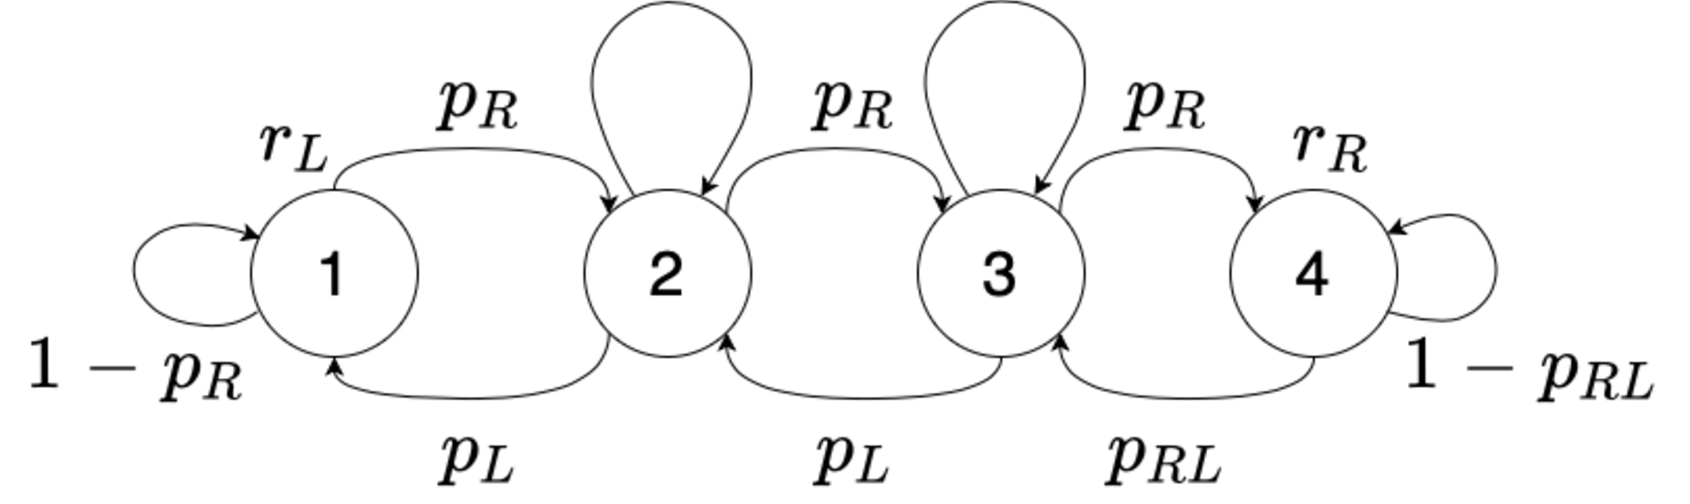
\includegraphics[angle=0, width=0.43\linewidth]{RandomWalk}    
        \end{tabular} \\
        \begin{tabular}{|@{~}c@{~}|@{~}c@{~}|@{~}c@{~}|@{~}c@{~}|@{~}c@{~}|c@{~}|@{~}c@{~}|@{~}c@{~}|@{~}c@{~}|}
            \cline{6-9}
            \multicolumn{5}{@{}c@{}}{} 
            & \multicolumn{4}{@{}|@{~}c@{~}| }{Gittins index for each state} \\ \cline{1-9}
             $p_L$ & $p_R$ & $p_{RL}$ & $r_L$ & $r_R$ & 1 & 2 & 3 & 4\\ \cline{1-9}
              0.1  &  0.2  &   0.3    &  0.2  &  1.0  & 0.276 & 0.2894 & 0.392 & 1.0 \\ \cline{1-9}
              0.1  &  0.5  &   0.7    & 0.35  &  0.7  & 0.35 & 0.256 & 0.2892 & 0.7 \\ \cline{1-9}
              0.1  &  0.4  &   0.5    &  0.4  &  0.65 & 0.4 & 0.250 & 0.286 & 0.65 \\ \cline{1-9}
            \end{tabular}            
    \end{tabular}
    \vspace{0.2cm}
    \caption{The random walk chain with 4 states. In state 4, the chain has an average reward $r_R$. For state 2 and 3, the chain gives zero reward. In state 1, the mean reward is $r_L$. This chain is obtained by applying the optimal policy on the 4-state river swim MDP of \cite{filippi2010optimism}. The table contains the parameters that we used, along with Gittins indices of all states when the discount factor is $\gamma=0.99$.}
    \label{fig:randomwalk}
\end{table}


\subsection{MB-PSRL}
\label{sssec:impl_gittinsPS}

MB-PSRL, the adaption from PSRL, puts prior distribution on the parameters $(\vr_a,\mP_a)$ of each Arm$~a$, draws a sample from the posterior distribution and uses it to compute the Gittins indices at the start of each episode. We implement two posterior updates for the mean reward vector $\vr_a$: Beta and Gaussian-Gamma. The second posterior, Gaussian-Gamma, will be used in prior choice sensitivity tests. For the transition matrix $\mP_a$, we implemented Dirichlet posterior update because Dirichlet distribution is the only natural conjugate prior for categorical distribution. Beta, Gaussian-Gamma and Dirichlet distributions can be easily sampled using the \texttt{numpy} package of Python. This greatly contributes to the computational efficiency of MB-PSRL.

We give more details on this prior distribution and their conjugate posterior in the subsections below.

\subsubsection{Bayesian Updates: Conjugate Prior and Posterior Distributions}
\label{apx:Bayes}

MB-PSRL is a Bayesian learning algorithm. 
As such, it samples reward vectors and transition matrices at the start each episode.
We would like to emphasize that neither the definition of the algorithm nor its performance guarantees that we prove in Theorem~\ref{thm:regret_upper_bound} depend on a specific form of the prior distribution $\phi$. 
Yet, in practice, some prior distributions are more preferable because their conjugate distributions are easy to implement. 
In the following, we give concrete examples on how to update the conjugate distribution given the observations. 

For $a\in[n]$ and $s_a\in\gS_a$, let $N^{k}(s_a)$ be the number of activations of arm $a$ while in state $s_a$ up to episode $k$. 
For this state $s_a$, the number of samples of the reward and of transitions from $s_a$ are equal to $N^{k}(s_a)$. 
To ease the exposition, we drop the label $a$ and assume that we are given: 
\begin{itemize}
    \item $N^{k}(s)$ \emph{i.i.d.} samples $\{Y_1,\dots,Y_{N^{k}(s)}\}$ of next states to which the arm transitioned from $s$.
    \item $N^{k}(s)$ \emph{i.i.d.} samples $\{R_1,\dots,R_{N^{k}(s)}\}$ of random immediate rewards earned while the arm was activated in state $s$
\end{itemize}
Each $Y_i$ is such that $\Proba{Y_i=s'}=P(s,s')$ and each $R_i$ is such that $\ex{R_i}=r(s)$. In what follows, we describe natural priors that can be used to estimate the transition matrix and the reward vector. 

\subsubsection{Transition Matrix}
If no information is known about the arm, the natural prior distribution is to consider the lines $P(s,\cdot)$ of the matrix as independent multivariate random variables uniformly distributed among all non-negative vectors of length $S$ that sum to $1$. 
This corresponds to a Dirichlet distribution of parameters $\alpha=(1\ \dots\ 1)$. 
For a given $s$, the variables $\{Y_1,\dots,Y_{N^{k}(s)}\}$ are generated according to a categorical distribution $\mP(s,\cdot)$. 
The Dirichlet distribution is self-conjugate with respect to the likelihood of a categorical distribution. 
So, the posterior distribution $\phi(\mP(s,\cdot)| Y_1,\dots,Y_{N^{k}(s)})$ is a Dirichlet distribution with parameters $\vc=(c_1\ \dots\ c_S)$ where $c_s'=1+\sum_{i=1}^{N^{k}(s)}\ind{Y_i=s'}$.

\subsubsection{Reward Distribution}
\label{apx:reward_post}

As for the reward vector, the choice of a good prior depends on the distribution of rewards. 
We consider two classical examples: Bernoulli and Gaussian.

\paragraph{Bernoulli distribution}
A classical case is to assume that the reward distribution of a state $s$ is Bernoulli with mean value $r(s)$.
A classical prior in this case is to consider that $\{r(s)\}_{\{s\in\gS\}}$ are \emph{i.i.d.} random variables following a uniform distribution whose support is $[0,1]$. 
The posterior distribution of $r(s)$ at time $t$ is the distribution of $r(s)$ conditional to the reward observations from state $s$ gathered up to time $t$. 
The posterior distribution $\phi(r(s)\mid R_1,\dots,R_{N^{k}(s)})$ is then a Beta distribution with parameters $(1+\sum_{i=1}^{N^{k}(s)}\ind{R_i=1}, 1+\sum_{i=1}^{N^{k}(s)}\ind{R_i=0})$. 
Recall that the Beta distribution is a special case of the Dirichlet distribution in the same way as the Bernoulli distribution is a special case of the Categorical distribution. 

\paragraph{Gaussian distribution}
We now consider the case of Gaussian rewards, and we assume that the immediate rewards earned in state $s$ are \emph{i.i.d.} Gaussian random variables of mean and variance $(r(s), \sigma^2(s))$. 
A natural prior for Gaussian rewards is to consider that $(r(s), \frac1{\sigma^2(s)})$ are \emph{i.i.d.} bivariate random variables where the marginal distribution of each $\frac{1}{\sigma^2(s)}$ is a Gamma distribution (it is a natural belief since the empirical variance of Gaussian has a chi-square distribution which is a special case of Gamma distribution). 
Conditioned on $\frac1{\sigma^2(s)}$, $r(s)$ follows a Gaussian distribution of variance $\sigma^2(s)$. 
We say that $(r(s), \frac1{\sigma^2(s)})$ has a Gaussian-Gamma distribution, which is self-conjugate with respect to a Gaussian likelihood (\emph{i.e.,} the likelihood of Gaussian rewards). 
So, given the reward observations, the marginal distribution of $\frac{1}{\sigma^2(s)}$ is still a Gamma distribution. 
$r(s)$ has Gaussian distribution conditioned on the reward observations and $\frac1{\sigma^2(s)}$. 
Indeed, let $\hat{r}(s)=\frac{1}{N^{k}(s)}\sum_{i=1}^{N^{k}(s)}R_i$ and $\hat{\sigma}^2(s)=\frac{1}{N^{k}(s)}\sum_{i=1}^{N^{k}(s)}\left(R_i-\hat{r}(s)\right)^2$ be the empirical mean and empirical variance of $R_i$. Then it can be shown that the posterior distribution of $\frac{1}{\sigma^2(s)}$ and $r(s)$ are:
\begin{align*}
    \frac{1}{\sigma^2(s)}\mid R_1,\dots,R_{N^{k}(s)}&{\sim} 
    \mathrm{Gamma}\bigg(\frac{N^{k}(s){+}1}{2}, \frac{1}{2}{+}\frac{N^{k}(s)\hat{\sigma}^2(s)}{2} {+}\frac{N^{k}(s)\hat{r}^2(s)}{2(N^{k}(s){+}1)}\bigg)\\
    r(x)\mid \frac1{\sigma^2(x)}, R_1,\dots,R_{N^{k}(x)}&{\sim} \mathcal{N}\left(\frac{N^{k}(s)\hat{r}(s)}{N^{k}(s)+1}, \frac{\sigma^2(s)}{N^{k}(s)+1}\right).
\end{align*}
For more details about the analysis of conjugate prior and posterior presented above as well as more conjugate distributions, we refer the reader to \cite{fink1997compendium,murphy2007conjugate}.

Notice that a reward that has a Gaussian distribution violates the property that all rewards are in $[0,1]$.
This could invalidate the bound on the regret of our algorithm proven in Theorem \ref{thm:regret_upper_bound}. 
Actually, it is possible to correct the proof to cover the Gaussian case by replacing the Hoeffding's inequality used in Lemma \ref{lem:concentration} by a similar inequality, also valid for sub-Gaussian random variables, see \cite{vershynin2018high}. 
In the experimental section (see \ref{ssec:prior}), we also show that a bad choice for the prior distribution of the reward (assuming a Gaussian distribution while the rewards are actually Bernoulli) does not alter too much the performance of the learning algorithm. 

\subsection{Experimental Methodology}
\label{ssec:experimental_methodo}

In our numerical experiment, we did 3 scenarios to evaluate the algorithms (scenario 2 and 3 are given in Appendix~\ref{apx:add_numerical}). In each scenario, we choose the discount factor $\gamma=0.99$ (which is classical) and we compute the regret over $K=3000$ episodes. The number of simulations varies over scenario depending on how the regret is computed. For each run, we draw a sequence of horizons $\{H^k\}_{k\in[3000]}$ from a geometric distribution of parameter $0.01$, and we run all algorithms for this sequence of time-horizons to remove a source of noise in the comparisons.  

For a given sequence of policies $\pi^k$, following \Eqref{eq:regretTraj}, the expected regret is $\ex{\sum_{k=1}^K\Delta^k(\vs_{t^k})}$ where $\Delta^k(\vs_{t^k})$ is the expected regret over episode $k$.
To reduce the variance in the numerical experiment, we compute
$\Delta^k(\vs_{t^k})=v^{\pi_*}_M(\vs_{t^k}) -v^{\pi^k}_M(\vs_{t^k})$.
For a given Markovian bandit problem and state $\vs$, the value $v^{\pi^*}_{M}(\vs)$ can be computed by using the retirement evaluation presented in Page~272 of \cite{whittle1996optimal}. It seems, however, that the same methodology is not applicable to compute the value function of an index policy that is not the Gittins policy. This means that while the policy $\pi^k$ is easily computable, we do not know of an efficient algorithm to compute its value $v^{\pi^k}_{M}(\vs)$. Hence, in our simulations, we will use two methods to compute the regret, depending on the problem size:
\begin{enumerate}
    \item (Exact method) Let $(r^{\pi}, P^{\pi})$ be the reward vector and transition matrix under policy $\pi$ (i.e. $\forall \vs, \vs'\in\gX, r^{\pi}(\vs)=r(\vs,\pi(\vs)), P^{\pi}(\vs,\vs')=P^{\pi(\vs)}(\vs, \vs')$ as defined in \Eqref{eq:defP}). Using the Bellman equation, the value function under policy $\pi$ is computed by
    \begin{equation}
        \label{eq:exact_value}
        v_{M}^{\pi}=(I-\gamma P^{\pi})^{-1}r^{\pi}.
    \end{equation}
    The matrix inversion can be done efficiently with the \texttt{numpy} package of Python. However, this takes $S^{2n}+2S^{n}$ of memory storage. Hence, when the number of states and arms are too large, the exact computation method cannot be performed. 

    \item (Monte Carlo method) In Scenario~2, the model has $n=9$ arms with $S=11$ states each, which makes the exact method inapplicable. In this case, it is still possible to compute the optimal policy and to apply Gittins index based algorithms but computing their value is intractable. In such a case, to measure the performance, we do 240 simulations for each algorithm and try to approximate $\Delta^k$ by
    \begin{equation}
        \label{eq:simulation_value}
        \hat{\Delta}^k=\frac1{\text{\#replicas}}\sum_{j=1}^{\text{\#replicas}}\sum_{t=1}^{H^{k,(j)}}\Big[r(s_{t,a^{*,(j)}_t}^{*,(j)}) -r(s_{t,a^{(j)}_t}^{(j)})\Big],
    \end{equation}
    where $H^{k,(j)}$ is the horizon of the $k$th episode of the $j$th simulation and $\{s_{t,a^{*,(j)}_t}^{*,(j)}\}$ and $\{s_{t,a^{(j)}_t}^{(j)}\}$ are the trajectories of the oracle and the agent respectively. The term oracle refers to the agent that knows the optimal policy $\pi^*$.
\end{enumerate}
Note that the expectation of \Eqref{eq:simulation_value} is equal to the value given in \Eqref{eq:exact_value} but \Eqref{eq:simulation_value} has a high variance. Hence, when applicable (Scenario~1~and~3) we use \Eqref{eq:exact_value} to compute the expected regret.

\section{Additional Numerical Experiments}
\label{apx:add_numerical}

\subsection{Scenario 1: Small Dimensional Example (Random Walk chain)}
\label{sssec:random_walk}

This scenario is explained in Appendix~\ref{apx:scene1} and the main numerical results are presented in Section~\ref{sec:numerical}. Here, we provide the result with error bars with respect to the random seed. In \figurename~\ref{fig:randomwalk_3b4s_errorbar}, the error bar size equals twice the standard deviation over 80 samples (each sample is a simulation with a given random seed and the random seeds are different for different simulations).

\begin{figure}[ht]
    \center
    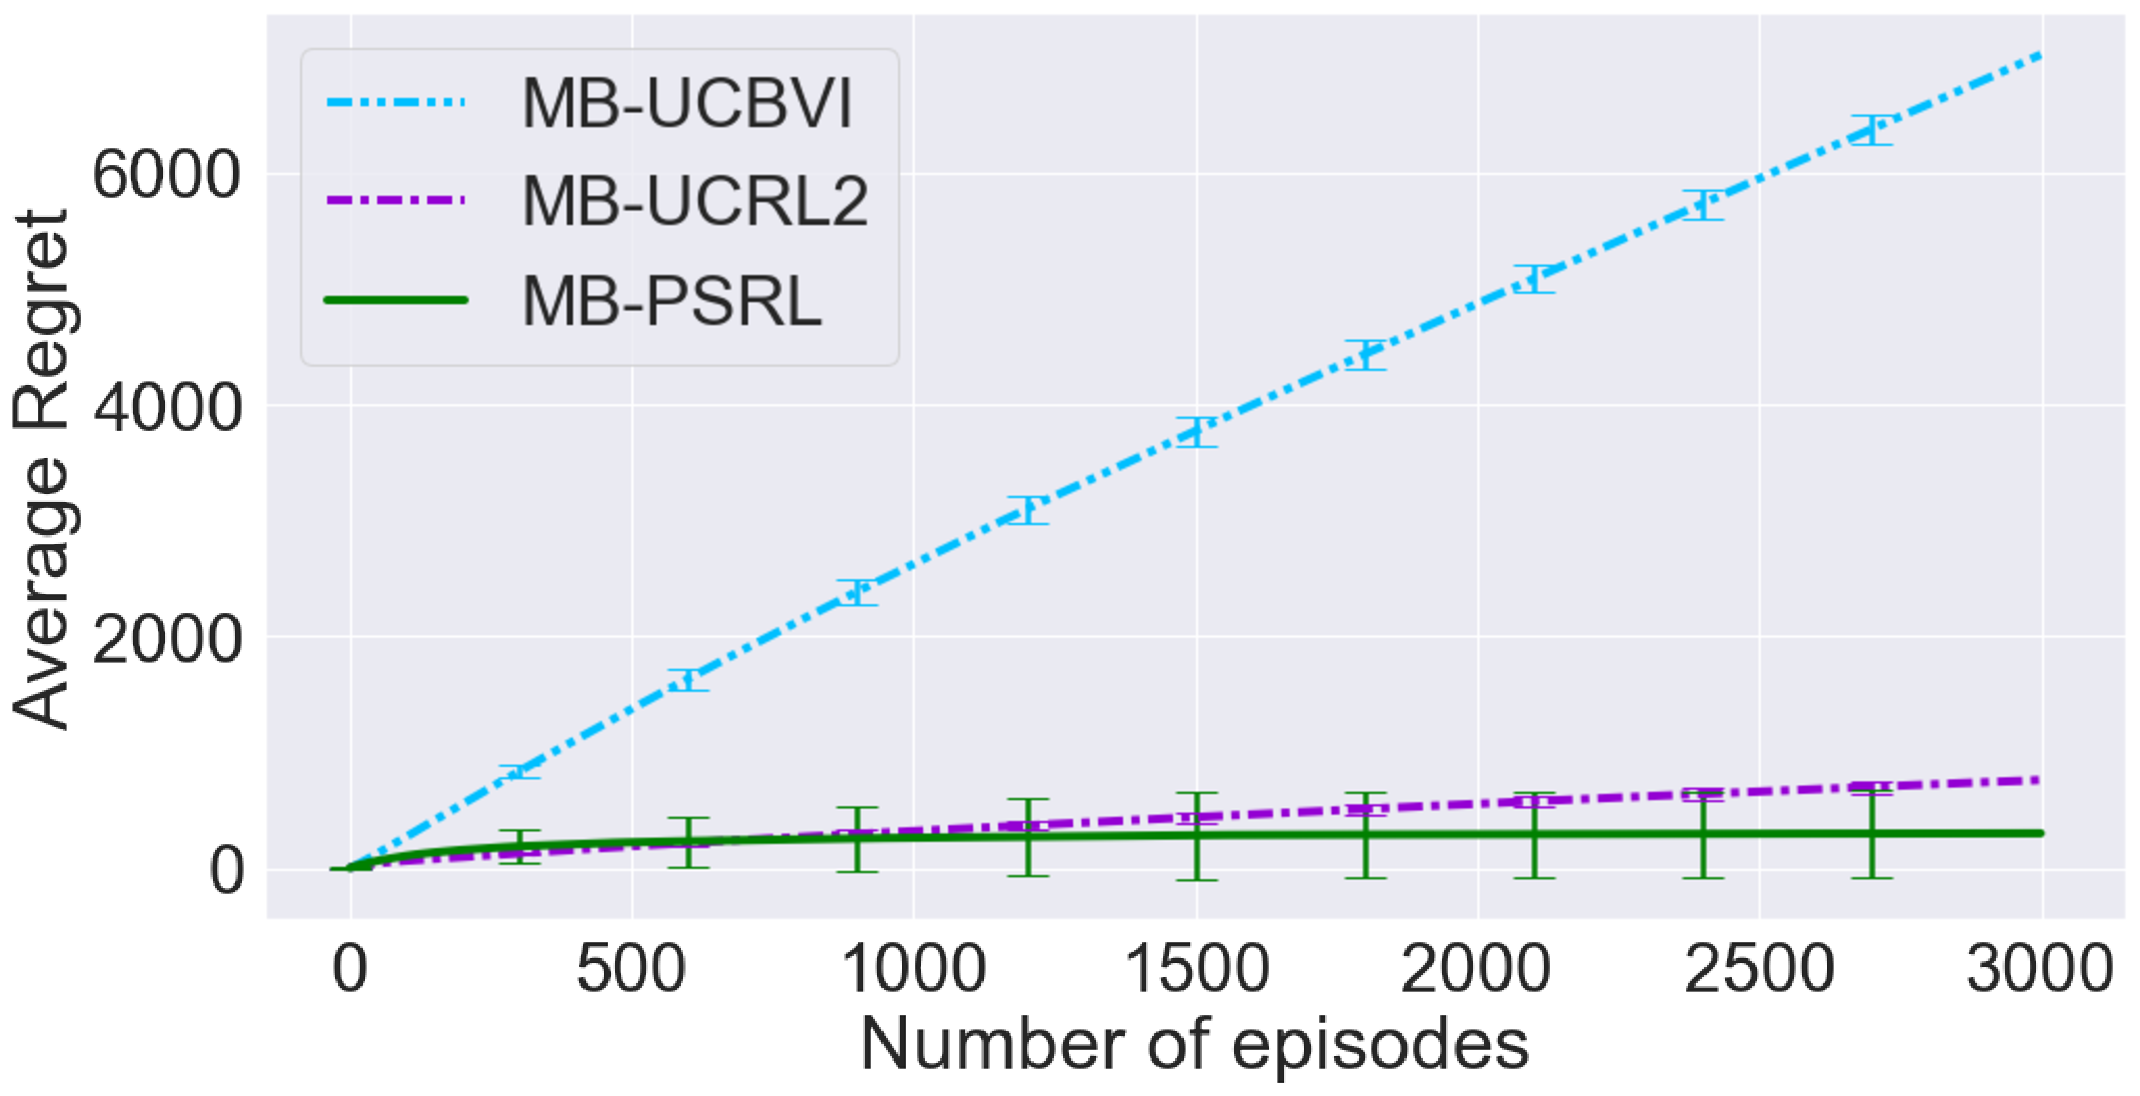
\includegraphics[width=0.9\linewidth]{3b4s_errorbar}
    \caption{Average cumulative regret in function of the number of episodes. Result from 80 simulations in a Markovian bandit problem with three 4-state random walk chains given in Table~\ref{fig:randomwalk}. The horizontal axis is the number of episodes. The size of the error bar equals twice the standard deviation over 80 simulations.}
    \label{fig:randomwalk_3b4s_errorbar}
\end{figure}

\subsection{Scenario 2: Higher Dimensional Example (Task Scheduling)}
\label{sssec:task_scheduling}

We now study an example that is too large to apply MB-UCRL2 . Hence, here we only compare MB-PSRL and MB-UCBVI. 

We implement the environment proposed on page 19 of \cite{duff1995q} that was used as a benchmark for the algorithm in the cited paper. Each chain represents a task that needs to be executed, and is represented in \figurename~\ref{fig:task_scheduling}(a). 
Each task has 11 states (including finished state $\star$ that is absorbing). 
For a given chain $a\in\{1,\dots,9\}$ and a state $i\in\{1,\dots,10\}$, the probability that a task $a$ ends at state $i$ is $\rho^{(a)}_{i}=\Proba{\tau^{(a)}=i \mid\tau^{(a)}\ge i}$ where $\tau^{(a)}$ is the execution time of task $a$. 
We choose the same values of the parameters as in \cite{duff1995q}: $\rho^{(a)}_{1}=0.1a$ for $a\in\{1,\dots,9\}$, $\lambda=0.8$, $\gamma=0.99$ and for $i\ge2$, 
\begin{align*}
    \mathbb{P}\{s_a=i\}=\left[1-[1-\rho^{(a)}_{1}]\lambda^{i-1}\right][1-\rho^{(a)}_{1}]^{i-1}\lambda^{\frac{(i-1)(i-2)}{2}}.
\end{align*}
Hence, the hazard rate $\rho^{(a)}_{i}$ is increasing with $i$. The reward in this scenario is deterministic: the agent receives 1 if the task is finished (\emph{i.e.,} under the transition from any state $i$ to state $\star$) and 0 otherwise (\emph{i.e.,} any other transitions including the one from state $\star$ to itself).
For MB-PSRL, we use a uniform prior for the expected rewards and consider that the rewards are Bernoulli distributed.

\begin{figure}[ht]
    \center
    \begin{tabular}{cc}
        \begin{minipage}{.5\linewidth}
            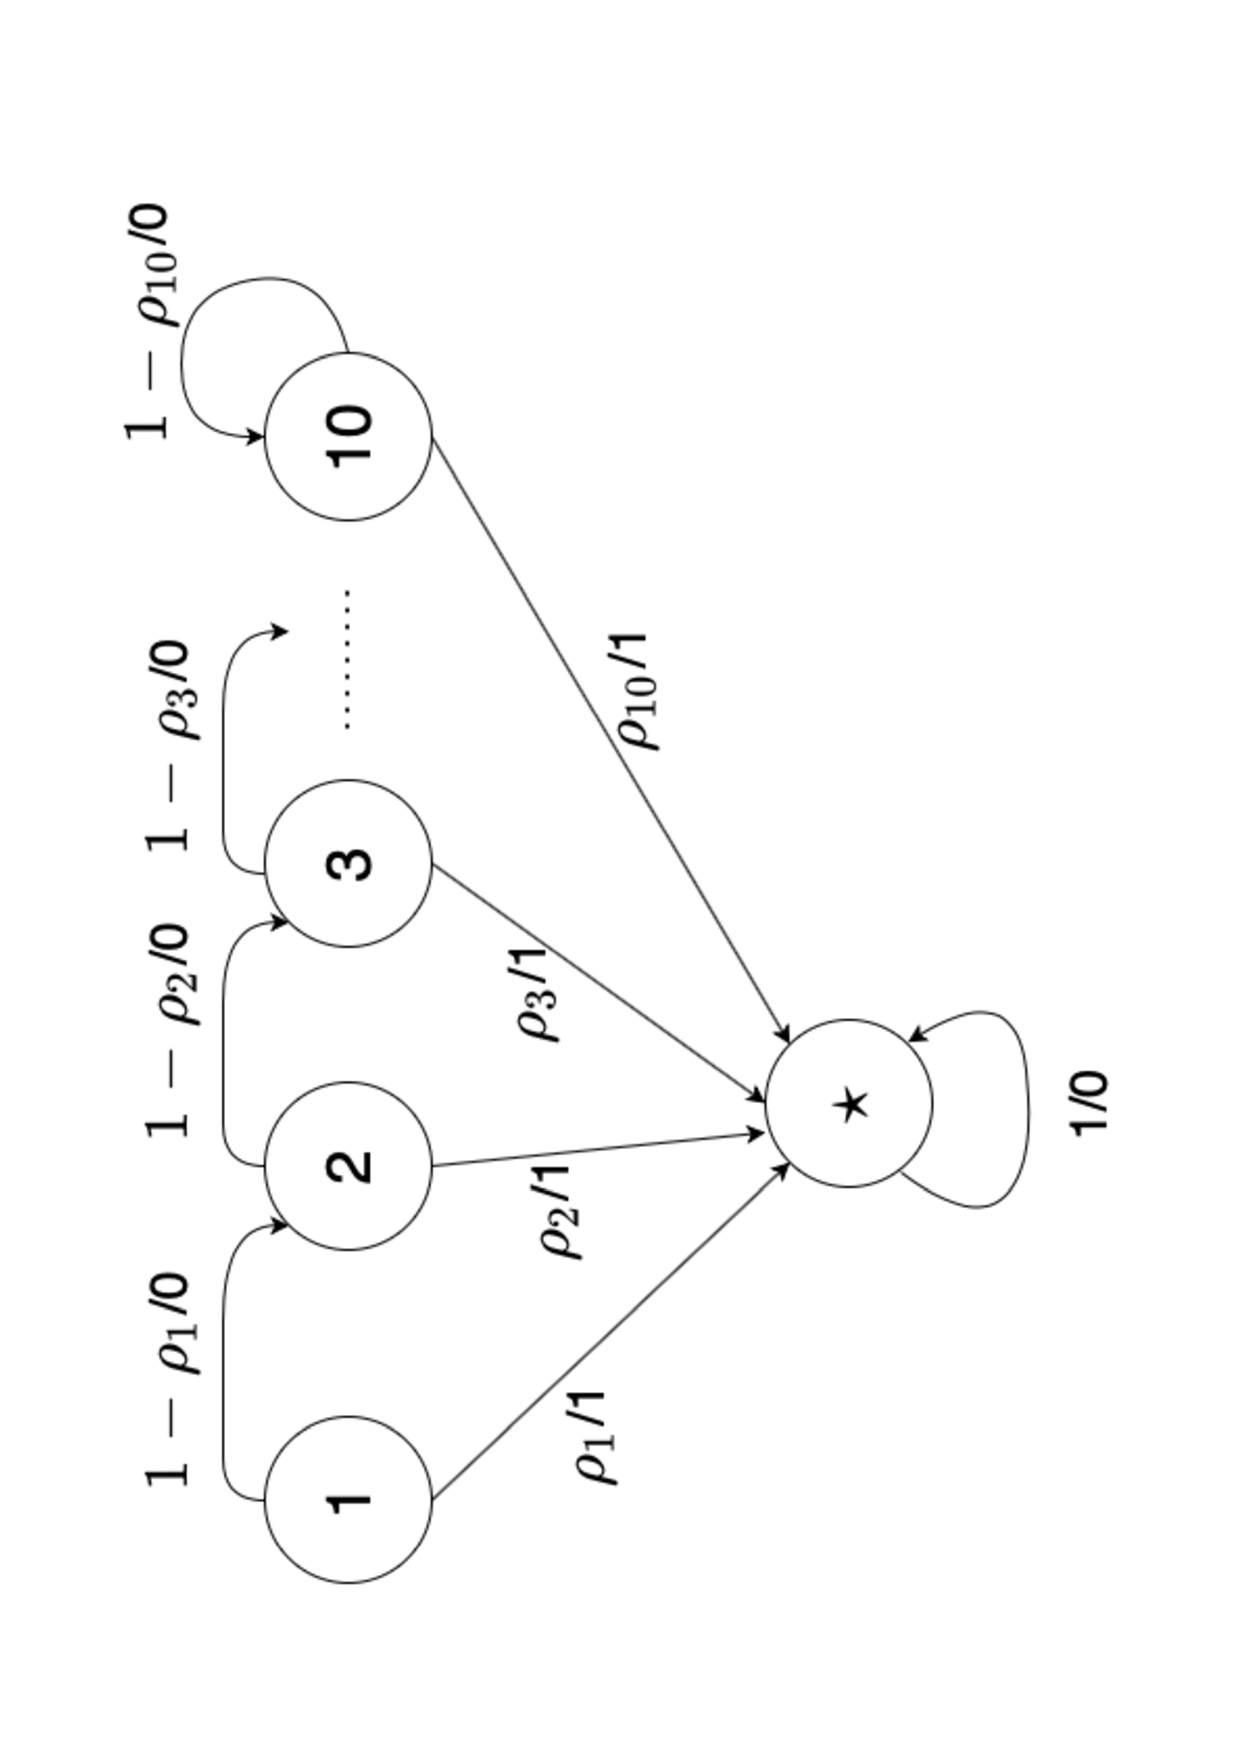
\includegraphics[angle=270, width=\textwidth]{Task_Scheduling}
            (a) In state $i$, the task is finished with probability $\rho_i$ or transitions to state $i+1$ with probability $1-\rho_i$. For $i=1,\dots,10$, the transition from state $i$ to state $\star$ provides 1 as the immediate reward. Otherwise, the agent always receives 0 reward.
        \end{minipage}
        &
        \begin{minipage}{.4\linewidth}
            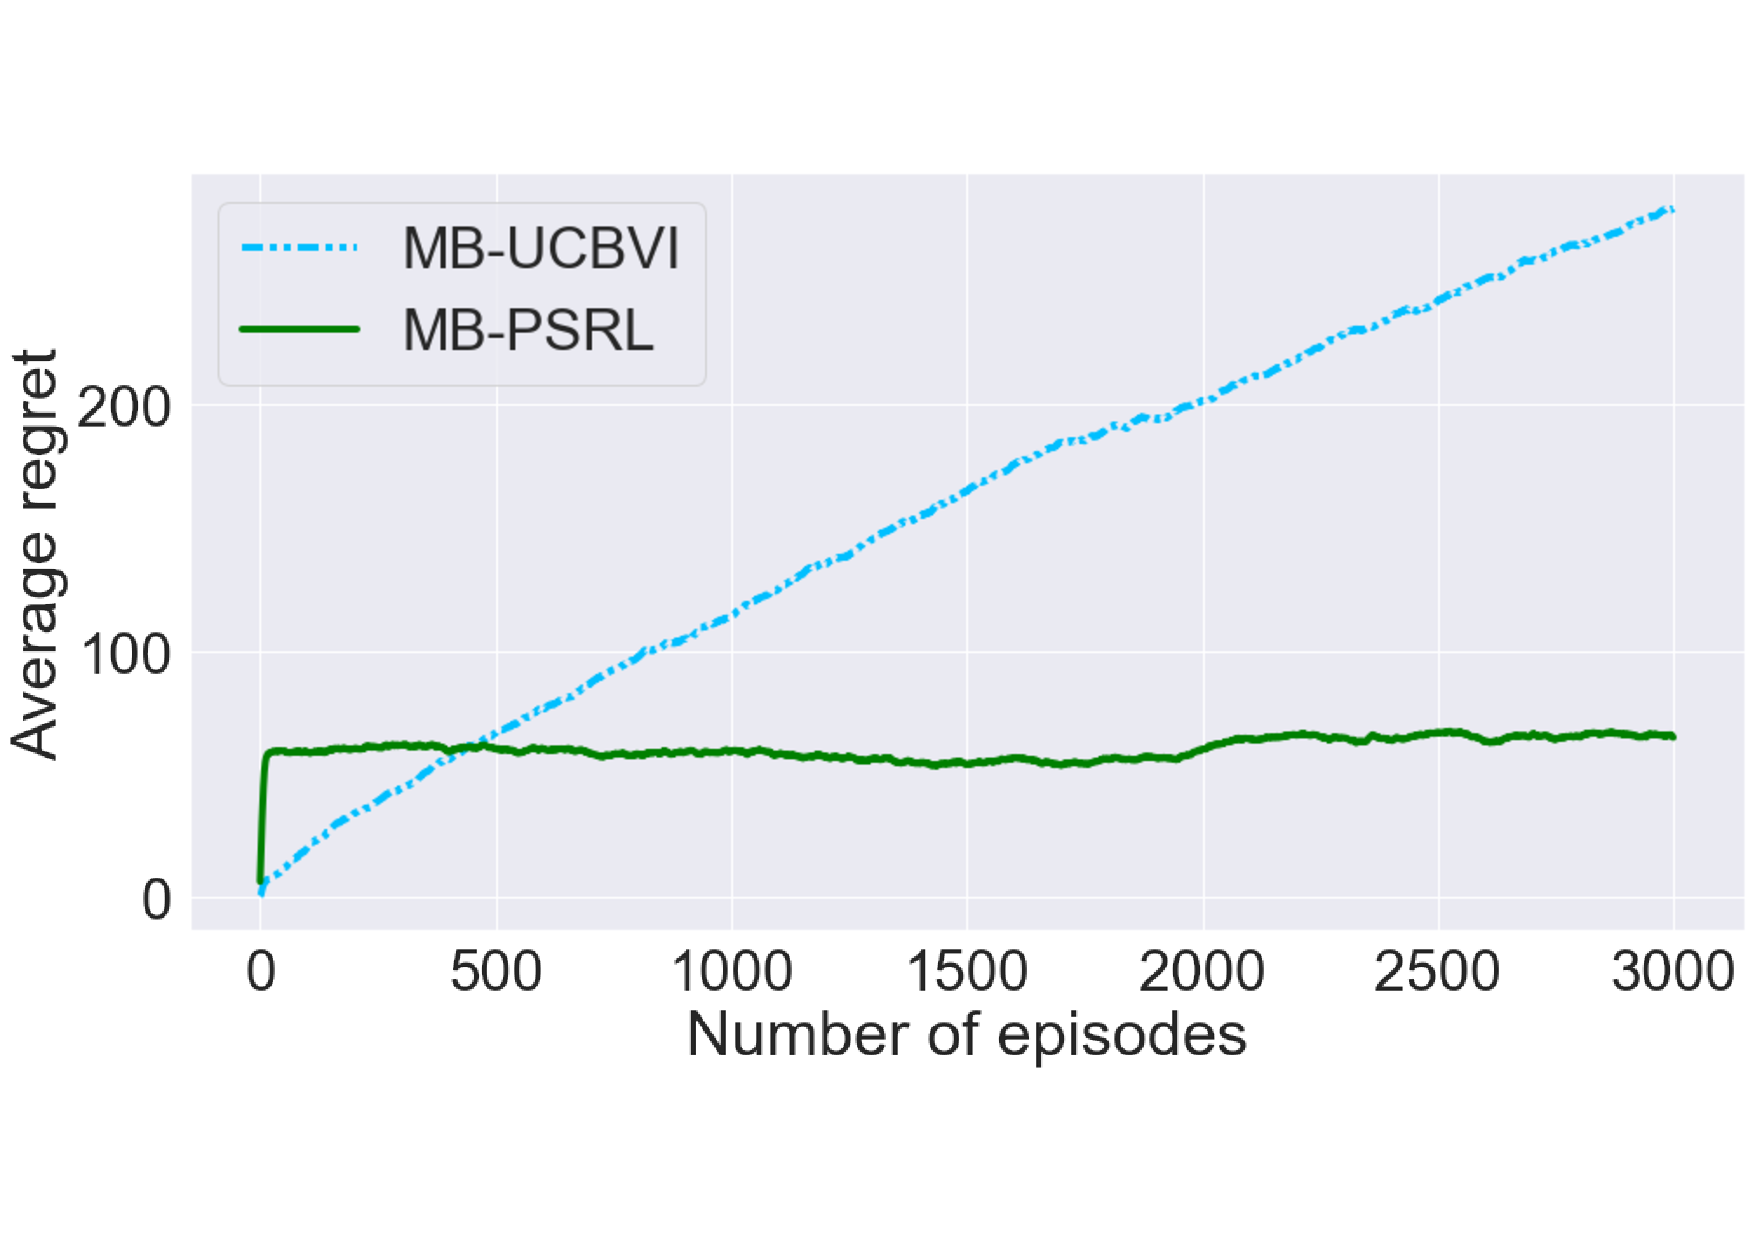
\includegraphics[angle=0, width=\columnwidth]{9b11s}
            (b) Average cumulative regret over 240 simulations.
        \end{minipage}        
    \end{tabular}
    \caption{Task Scheduling with 11 states including the absorbing state (finished state). }
    \label{fig:task_scheduling}
    %\Description{Markov chain from Duff (1995).}
\end{figure}


The average regret of the two algorithms is displayed in \figurename~\ref{fig:task_scheduling}(b). As before, MB-PSRL outperforms MB-UCBVI.  Note that we also studied the time to run one simulation for 3000 episodes. This time is around 1 min for MB-PSRL and MB-UCBVI. 

\subsection{Scenario 3: Bayesian Regret and Sensitivity to the Prior}
\label{ssec:prior}

In this section, we study how robust the two implementations of PSRL are, namely MB-PSRL and vanilla PSRL (to simplify, we will just call the latter PSRL), to a choice of prior distributions. 
As explained in Appendix~\ref{apx:reward_post}, the natural conjugate prior for Bernoulli reward is the Beta distribution. 
In this section, we simulate MB-PSRL and PSRL in which the rewards are Bernoulli but the conjugate prior used for the rewards are Gaussian-Gamma which is incorrect for Bernoulli random reward. 
In other words, MB-PSRL and PSRL have Gaussian-Gamma prior belief while the real rewards are Bernoulli random variables. 


To conduct our experiments, we use a Markovian bandit problem with three $4$-state random walk chains represented in Table~\ref{fig:randomwalk}. 
We draw 16 models by generating 16 pairs of $(r_L, r_R)$ from $U[0,1]$, 16 pairs of $(p_L, p_R)$ from Dirichlet(3,(1,1,1)) and 16 values of $p_{RL}$ from Dirichlet(2, (1,1)) for each chain. 
Each model is an unknown MDP that will be learned by MB-PSRL or PSRL. 
For each of these $16$ models, we simulate MB-PSRL and PSRL 5 times with correct priors and 5 times with incorrect priors. 
The result can be found in \figurename~\ref{fig:bayes_gittinsPS} which suggests that MB-PSRL performs better when the prior is correct and is relatively robust to the choice of priors in terms of Bayesian regret. 
This figure also shows that PSRL seems more sensitive to the choice of prior distribution. 
Also note that for both MB-PSRL and PSRL, some trajectories deviate a lot from the mean, under correct priors but even more so with  incorrect priors. 
This illustrates the general fact that learning can go wrong, but with a small probability.

\begin{figure*}[tb]
    \begin{tabular}{cccc}
        \rotatebox{90}{\quad\qquad MB-PSRL}
        &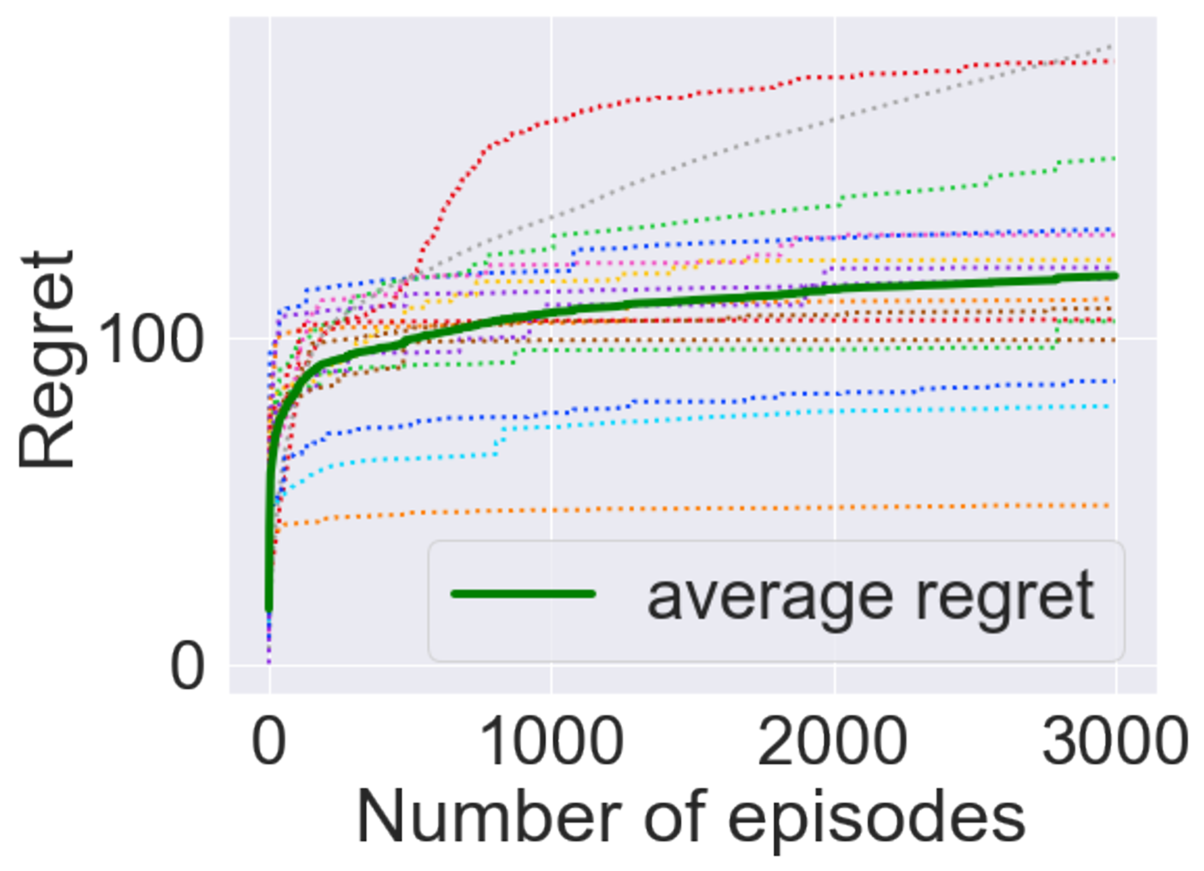
\includegraphics[width=0.3\linewidth]{gittinsPS_corr_prior}
        &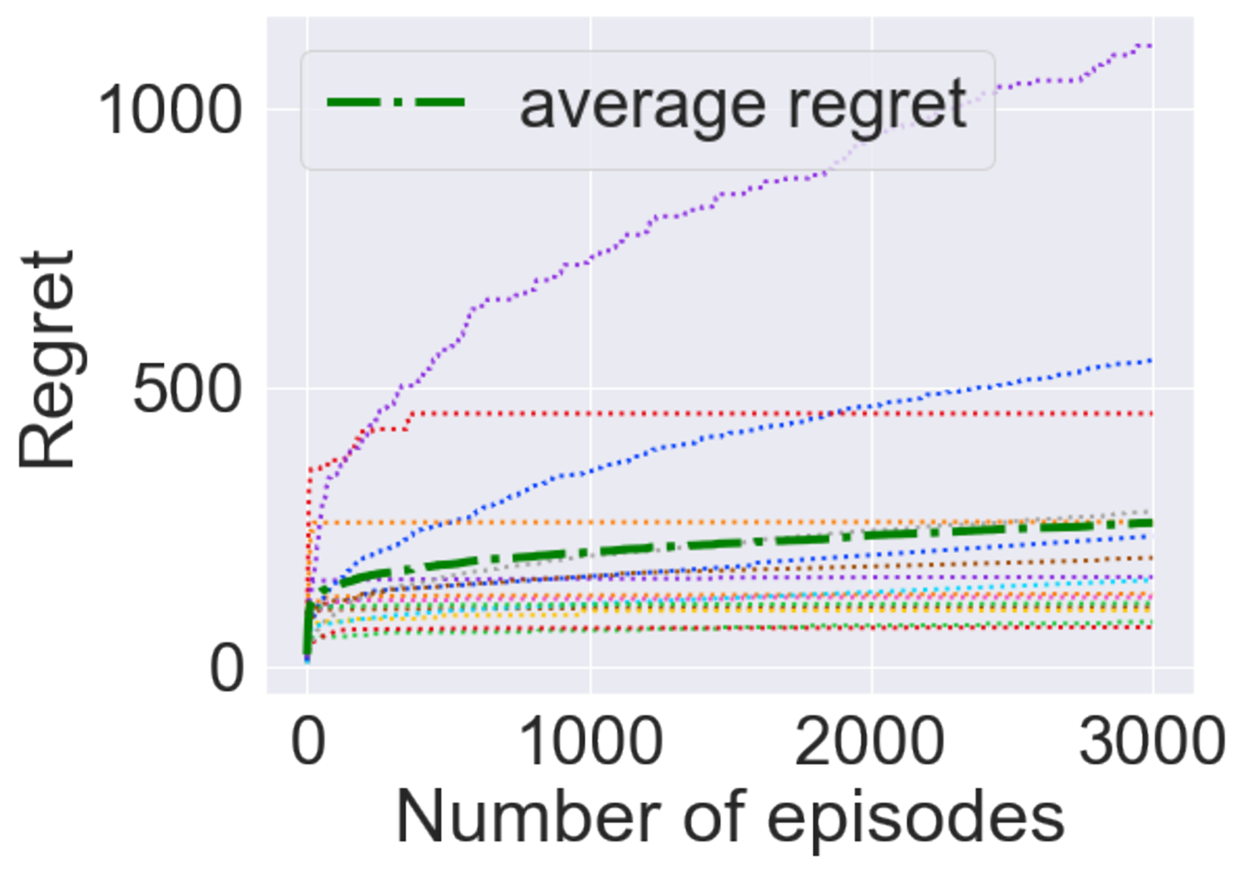
\includegraphics[width=0.3\linewidth]{gittinsPS_incorr_prior}
        &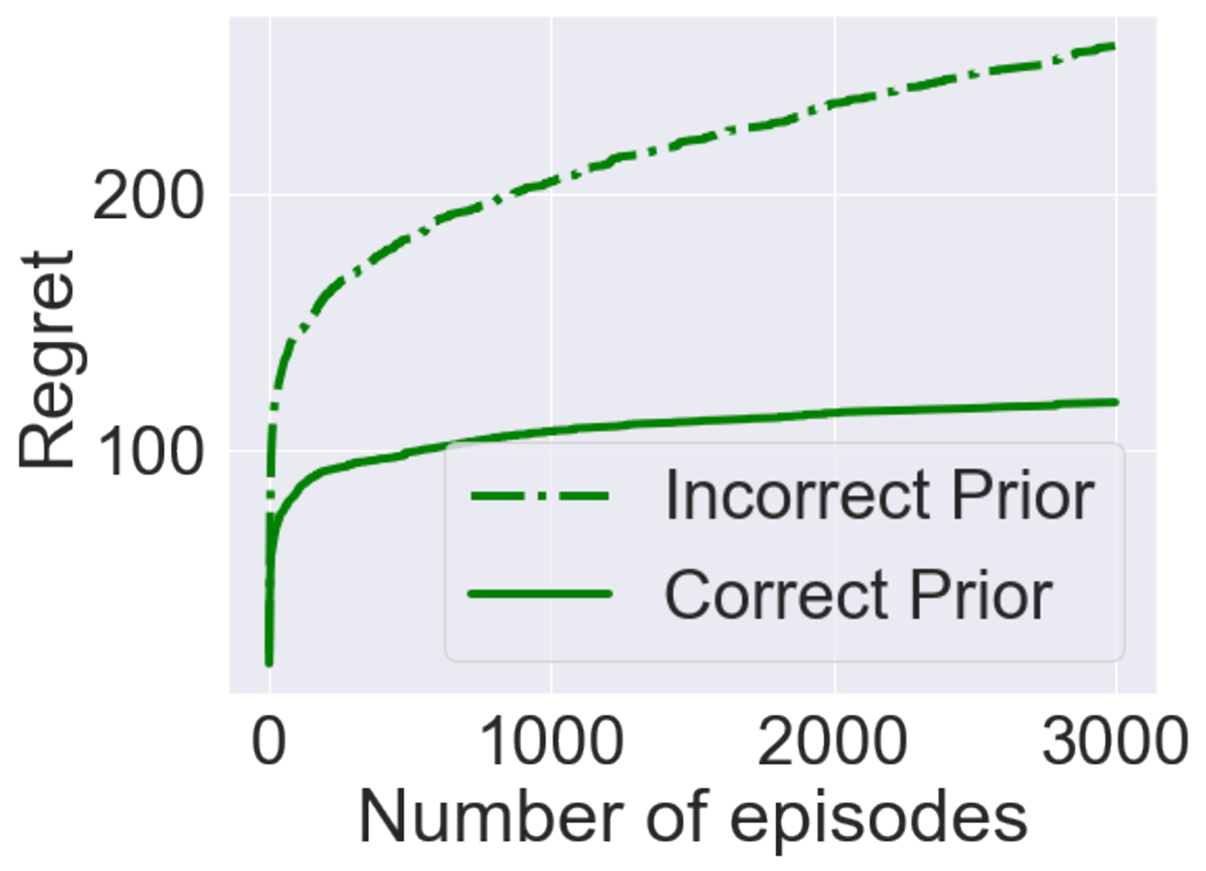
\includegraphics[width=0.3\linewidth]{gittinsPS_prior_choices}\\
        \rotatebox{90}{\qquad\qquad PSRL}
        &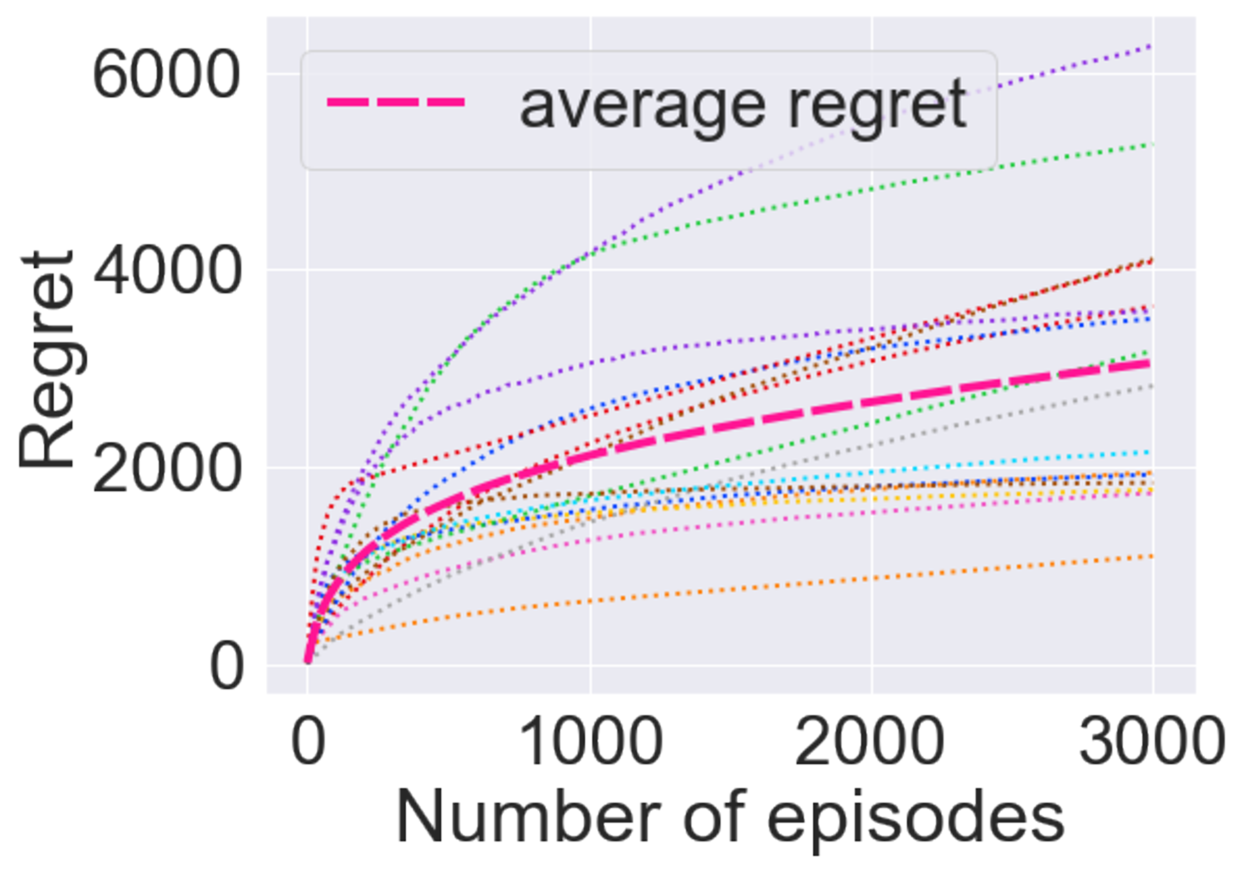
\includegraphics[width=0.3\linewidth]{PSRL_corr_prior}
        &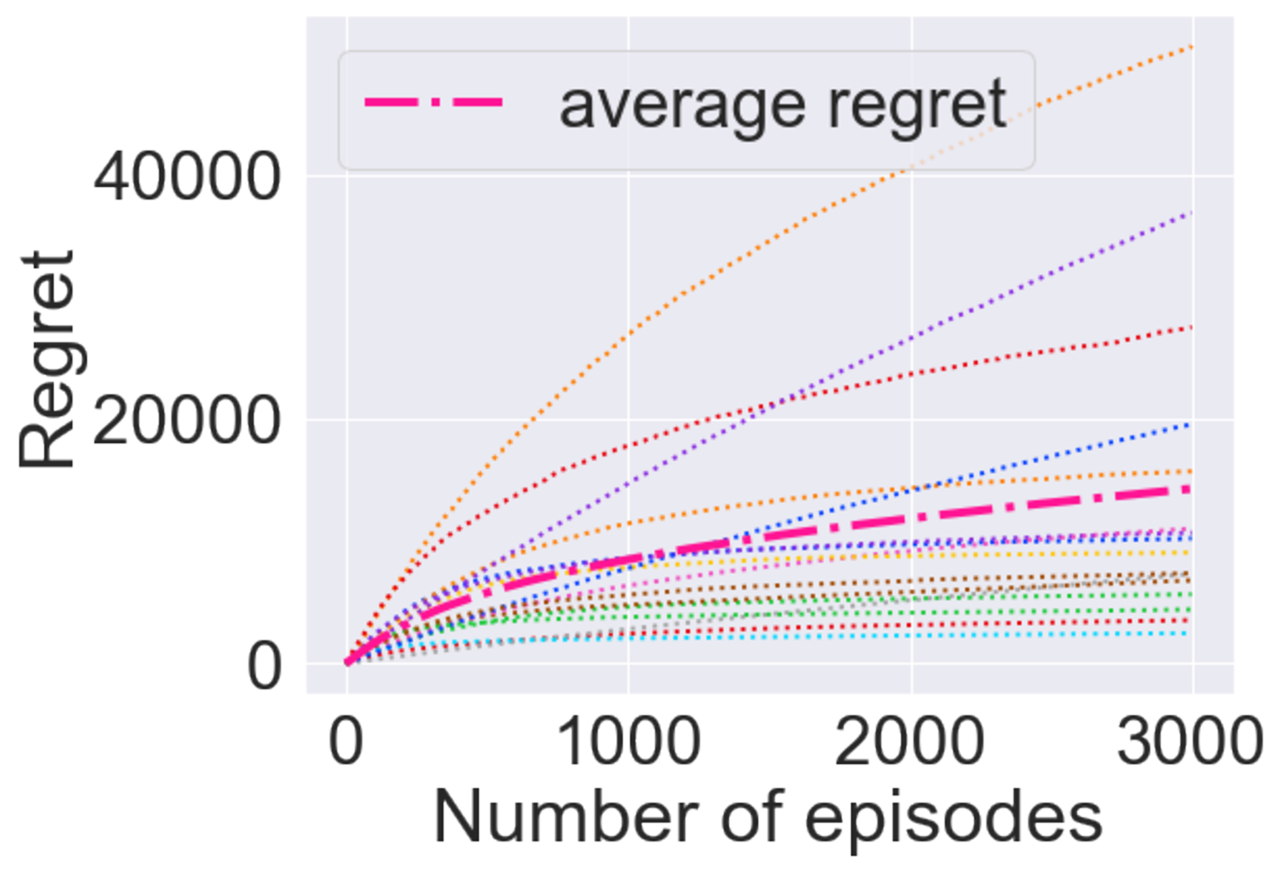
\includegraphics[width=0.3\linewidth]{PSRL_incorr_prior}
        &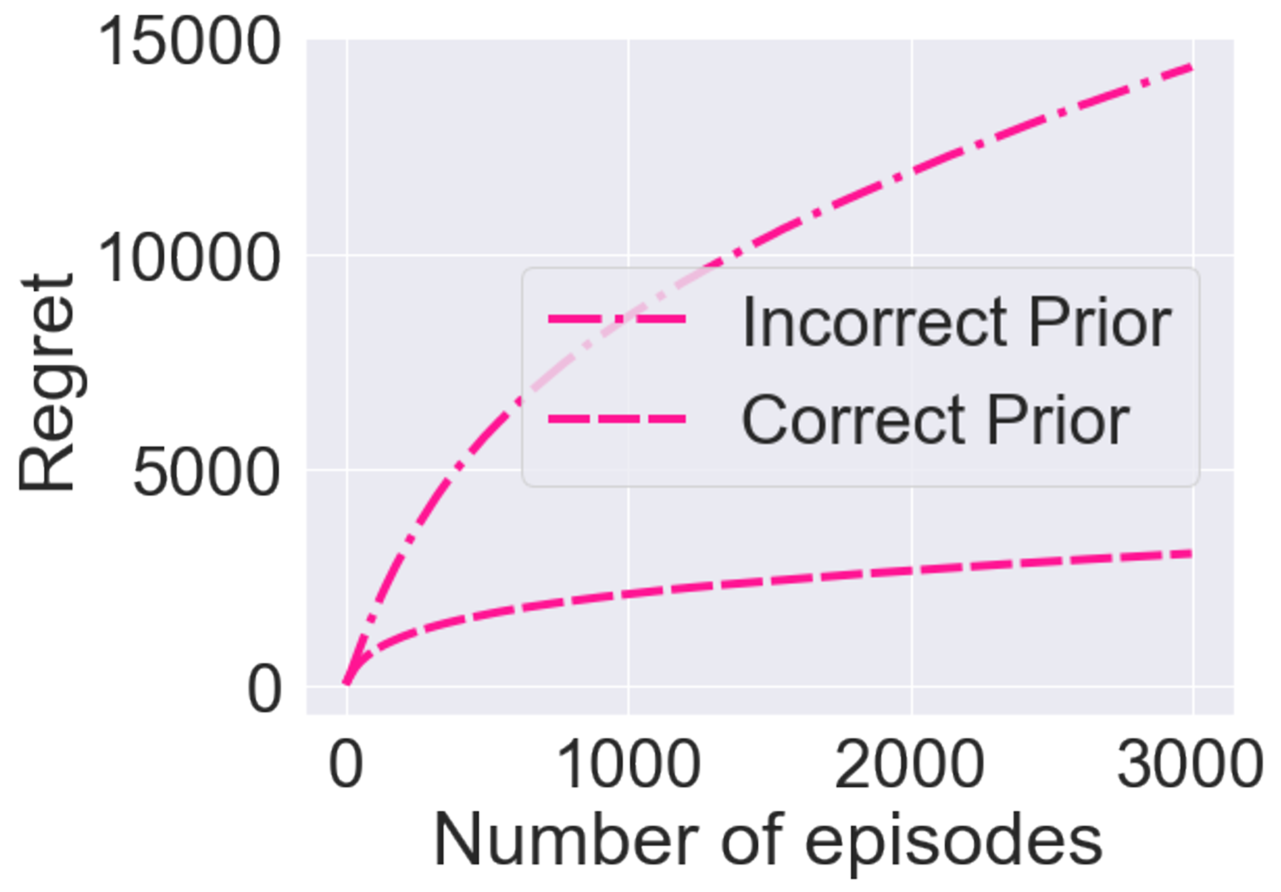
\includegraphics[width=0.3\linewidth]{PSRL_prior_choices}\\
        &\begin{subfigure}[b]{0.3\linewidth}\caption{Correct Prior}\label{subfig:gittinsPS_corr_prior}\end{subfigure}
        &\begin{subfigure}[b]{0.3\linewidth}\caption{Incorrect Prior}\label{subfig:gittinsPS_incorr_prior}\end{subfigure}
        &\begin{subfigure}[b]{0.3\linewidth}\caption{Bayesian Regret}\label{subfig:gittinsPS_prior_choices}\end{subfigure}
    \end{tabular}
    \caption{Bayesian regret of MB-PSRL and vanilla PSRL in 3 4-state Random Walk chains. For each chain, we draw 16 random models and run the algorithms for 5 simulations in each model (there are 80 simulations in total). In panels (a) and (b), we plot 16 dotted lines that correspond to the average cumulative regret over 5 simulations in the 16 samples. The solid and dash-dot lines are the average regret each over 80 simulations (the estimated Bayesian regret). \figurename~\ref{subfig:gittinsPS_corr_prior} shows the performance when reward prior is well-chosen (namely, $U([1,1])$). \figurename~\ref{subfig:gittinsPS_incorr_prior} is when the reward prior is incorrectly chosen (namely Gaussian-Gamma distribution). \figurename~\ref{subfig:gittinsPS_prior_choices} compares the Bayesian regret of the correct prior with the incorrect one (dash-dot line). In both case, the prior of next state transition is well-chosen (namely, Dirichlet distribution). Y-axis range changes for each figure.}
    \label{fig:bayes_gittinsPS}
\end{figure*}


\section{Experimental environment}
\label{apx:envi}

The code of all experiments is given in a separated zip file that contains all necessary material to reproduce the simulations and the figures. 

Our experiments were run on HPC platform with 1 node of 16 cores of Xeon E5. The experiments were made using Python 3 and Nix and submitted as supplementary material and will be made publicly available with the full release of the paper. The package requirement is detailed in README.md. Using only \emph{1 core} of Xeon E5, the Table~\ref{tab:sim_time} gives some orders of duration taken by each experiment (with discount factor $\gamma=0.99$, and 3000 episodes per simulation). We would like to draw two remarks. First, the duration reported in Figure~\ref{fig:randomwalk_cpt_3b4s} is the time for policy computation (algorithm's parameters update and policy computation). The duration reported in Table~\ref{tab:sim_time} includes this plus the computation time for oracle (because we track the regret), the state transition time along the trajectories of oracle and of each algorithm, resetting time... This explains why the duration reported in Table~\ref{tab:sim_time} cannot be compared to the duration reported in Figure~\ref{fig:randomwalk_cpt_3b4s}.  Second, the duration shown in Table~\ref{tab:sim_time} are meant to be a rough estimation of the computation time (we only ran the simulation once and the average duration might fluctuate). 

\begin{table}[ht]
    \centering
    \begin{tabular}{ |c|c|c|c|c|c| } 
    \hline
    Experiment & MB-PSRL  & PSRL & MB-UCRL2 & MB-UCBVI & Total\\
    \hline
    Scenario 1 & 40 min  & - & 6 days & 50 min & 6 days\\ 
    \hline
    Scenario 2 & 200 min  & - & - & 200 min & 400 min\\ 
    \hline
    Scenario 3 & 90 min  & 260 min & - & - & 350 min\\ 
    \hline
    \end{tabular}
\vspace{0.2cm}
\caption{Approximative execution time for simulating each algorithm and tracking its regret in each scenario. This time includes the time given in Figure~\ref{fig:randomwalk_cpt_3b4s} and the computation time needed by oracle (because we track the regret), the state transition time along the trajectories of oracle and each algorithm, etc. In each scenario, we set the discount factor $\gamma=0.99$ and run the algorithms for $3000$ episodes per simulation.}
\label{tab:sim_time}
\end{table}

\end{subappendices}

\endgroup
